\documentclass[12pt,a4paper,openany]{book}

% Librerias

\usepackage{babel}
\babelprovide[main,import]{spanish}
\usepackage[utf8]{inputenc}
\usepackage[T1]{fontenc}
\usepackage[sfdefault,scale=0.96]{plex-sans}
\usepackage[scale=0.91]{plex-mono}

% Ajustes de espaciado y expansión disponibles en pdfTeX.
\AtBeginDocument{%
  \ifdefined\pdffontexpand
  \pdffontexpand\font 25 25 1 autoexpand
  \pdfadjustspacing=2
  \fi
}
\clubpenalty=10000
\widowpenalty=10000
\displaywidowpenalty=10000

\usepackage{amsmath, amssymb}
\usepackage{siunitx}
\sisetup{
  output-decimal-marker = {,},
  inter-unit-product = \cdot,
  exponent-product = \cdot,
  per-mode = symbol
}

\usepackage{tabularx}
\usepackage{booktabs}
\setlength{\extrarowheight}{2pt}
\renewcommand{\arraystretch}{1.18}
\newcolumntype{Y}{>{\raggedright\arraybackslash}X}
\newcolumntype{Z}{>{\centering\arraybackslash}X}
\newcolumntype{L}[1]{>{\raggedright\arraybackslash}p{#1}}
\newcolumntype{C}[1]{>{\centering\arraybackslash}p{#1}}
\usepackage{float}
\usepackage{needspace}

\usepackage{graphicx}
\usepackage{caption}
\captionsetup[figure]{justification=centering, singlelinecheck=false}
\captionsetup[table]{justification=centering, singlelinecheck=false}
\renewcommand{\tablename}{Tabla}
\addto\captionsspanish{\renewcommand{\tablename}{Tabla}}

\usepackage[top=2.5cm, bottom=2.5cm, left=1.5cm, right=1.5cm]{geometry}
\raggedbottom
\setlength{\emergencystretch}{0.5em}
\tolerance=1800
\setlength{\parskip}{0.55em}

\usepackage{xcolor}
\definecolor{codeback}{RGB}{252,251,255}
\definecolor{coderule}{RGB}{218,212,232}
\definecolor{codeviolet}{RGB}{109,78,180}
\definecolor{codeblue}{RGB}{48,97,171}
\definecolor{codestring}{RGB}{38,127,118}
\definecolor{codecomment}{RGB}{118,124,132}
\definecolor{codenumber}{RGB}{142,134,164}
\definecolor{technicalviolet}{RGB}{98,64,150}
\definecolor{placeholdergray}{RGB}{248,248,248}
\definecolor{placeholderline}{RGB}{160,160,160}

\DeclareTextFontCommand{\texttt}{\ttfamily\color{technicalviolet}}
\newcommand{\tech}[1]{\mbox{\texttt{#1}}}
% Nombres técnicos con guiones bajos sin escape manual.
\newcommand{\code}[1]{\texttt{\detokenize{#1}}}
% Enlaces fijados: el PDF debe poder consultarse fuera del checkout.
\newcommand{\projecturl}{https://github.com/FrancoPerotti/computer-architecture-tps}
\newcommand{\baserevision}{7025925f949c16cbe1a5bd44bf17d9e9ed01a78c}
\newcommand{\acceptancerevision}{cb3270b19b2721f3e72a23ab23e333b394d113b9}
\newcommand{\doc}[2]{\href{\projecturl/blob/\baserevision/tp3/docs/#1}{#2}}
\newcommand{\acceptancedoc}[1]{\href{\projecturl/blob/\acceptancerevision/tp3/docs/verification/board_acceptance.md}{#1}}
\newcommand{\evidencefile}[2]{\href{\projecturl/releases/download/tp3-17-evidencia/#1}{#2}}
\graphicspath{{img/}{diagrams/pdf/}{../../tp2/informe/img/}{../docs/diagrams/previews/}}

\usepackage{listings}
\lstdefinelanguage{SystemVerilog}{
  morekeywords={module,endmodule,input,output,wire,reg,logic,parameter,localparam,integer,
    always,always_comb,posedge,negedge,begin,end,if,else,case,endcase,default,
  task,endtask,automatic,initial,repeat,for,signed,assign},
  sensitive=true,
  morecomment=[l]{//},
  morecomment=[s]{/*}{*/},
  morestring=[b]"
}
\lstdefinelanguage{bash}{
  morekeywords={make, cd, docker, npm, node, bash, python3, pdflatex, chktex},
  sensitive=true,
  morecomment=[l]{\#},
  morestring=[b]",
  morestring=[b]'
}
\lstdefinelanguage{RISCV}{
  morekeywords={lw, sw, lb, lh, lbu, lhu, sb, sh, add, sub, addi, and, or, xor,
    sll, srl, sra, slli, srli, srai, beq, bne, jal, jalr, lui, halt},
  sensitive=true,
  morecomment=[l]{//}
}
\lstdefinestyle{tpcode}{
  basicstyle=\ttfamily\small\color{black!88},
  breaklines=true,
  columns=fullflexible,
  commentstyle=\color{codecomment}\itshape,
  keywordstyle=\color{codeviolet}\bfseries,
  morekeywords={module_init,module_exit,THIS_MODULE,KERN_INFO,KERN_ERR,NULL,true,false,None,global,with,as,return,try,except,while,if,else,elif},
  emph={always_comb,urandom,fatal,display,finish,signed,ASYNC_REG,create_clock,set_false_path},
  emphstyle=\color{codeblue},
  stringstyle=\color{codestring},
  frame=none,
  keepspaces=true,
  lineskip=0.5pt,
  numbers=none,
  numberstyle=\scriptsize\ttfamily\color{codenumber},
  showstringspaces=false,
  tabsize=2
}
\lstset{style=tpcode}
\usepackage[skins,breakable,listings]{tcolorbox}
\usetikzlibrary{positioning,arrows.meta,fit}
\newtcblisting{codebox}[1][]{
  listing only,
  enhanced,
  colback=codeback,
  colframe=coderule,
  boxrule=0.45pt,
  borderline west={2.8pt}{0pt}{codeviolet},
  arc=2mm,
  boxsep=0pt,
  left=10pt,
  right=10pt,
  top=6pt,
  bottom=6pt,
  before skip=0.8em,
  after skip=0.9em,
  drop fuzzy shadow=black!8!white,
  listing options={style=tpcode,#1}
}

\usepackage{fancyhdr}
\pagestyle{fancy}
\setlength{\headheight}{14.5pt}

\usepackage{tocloft}
\setlength{\cftbeforechapskip}{0.42em}
\setlength{\cftbeforesecskip}{0.08em}
\setlength{\cftchapindent}{0pt}
\setlength{\cftsecindent}{1.35em}
\setlength{\cftchapnumwidth}{2.1em}
\setlength{\cftsecnumwidth}{2.8em}
\renewcommand{\cftchapfont}{\bfseries}
\renewcommand{\cftchappagefont}{\bfseries}
\renewcommand{\cftchapleader}{\cftdotfill{\cftdotsep}}
\renewcommand{\cfttoctitlefont}{\huge\bfseries}
\setlength{\cftbeforetoctitleskip}{-1.2em}
\setlength{\cftaftertoctitleskip}{1.0em}

\usepackage[colorlinks=true,
  linkcolor=black,
  citecolor=black,
  urlcolor=codeblue,
  filecolor=codeblue,
  menucolor=black]{hyperref}
\hypersetup{
  pdftitle={RISC-V con pipeline de cinco etapas},
  pdfauthor={Arnaudo, Federico Andres; Perotti, Franco Jose},
  pdfsubject={Trabajo Practico Numero 3 - Arquitectura de Computadoras},
  pdfkeywords={RISC-V, pipeline, Basys 3, UART, FPGA}
}
\Urlmuskip=0mu plus 1mu\relax
\fancyhead{}
\fancyhead[L]{UNC \textperiodcentered{} FCEFyN}
\fancyhead[R]{Arquitectura de Computadoras}
\fancyfoot{}
\fancyfoot[C]{\thepage}
\fancypagestyle{plain}{
  \fancyhead{}
  \fancyhead[L]{UNC \textperiodcentered{} FCEFyN}
  \fancyhead[R]{Arquitectura de Computadoras}
  \fancyfoot{}
  \fancyfoot[C]{\thepage}
}

% Reduce el espacio vertical excesivo que la clase book agrega antes
% de cada seccion.
\makeatletter
\renewcommand{\@seccntformat}[1]{\csname the#1\endcsname\hspace{0.75em}}
\renewcommand{\chaptername}{Sección}
\renewcommand{\@chapapp}{Sección}
\def\@makechapterhead#1{%
  \vspace*{-28\p@}%
  {\parindent \z@ \raggedright \normalfont
    \ifnum \c@secnumdepth >\m@ne
    \Large\bfseries \@chapapp\space \thechapter
    \par\nobreak
    \vskip 3\p@
    \fi
    \huge \bfseries #1\par\nobreak
    \vskip 4\p@
}}
\def\@makeschapterhead#1{%
  \vspace*{-28\p@}%
  {\parindent \z@ \raggedright
    \normalfont
    \huge \bfseries #1\par\nobreak
    \vskip 4\p@
}}
\renewcommand
\section{%
  \@startsection{section}{1}{\z@}%
  {-2.0ex \@plus -0.5ex \@minus -0.2ex}%
  {0.35em}%
  {\normalfont\Large\bfseries}%
}
\renewcommand
\subsection{%
  \@startsection{subsection}{2}{\z@}%
  {-1.6ex \@plus -0.4ex \@minus -0.2ex}%
  {0.25em}%
  {\normalfont\large\bfseries}%
}
\makeatother


\begin{document}

\begin{titlepage}
  \thispagestyle{empty}
  \sffamily
  \setlength{\parindent}{0pt}

  \begin{tikzpicture}[remember picture,overlay]
    \fill[technicalviolet] (current page.north west) rectangle
    ([xshift=0.34cm]current page.south west);
    \fill[codeback] ([xshift=0.34cm]current page.north west) rectangle
    (current page.south east);
  \end{tikzpicture}

  \vspace*{-0.2cm}
  \noindent
  \begin{minipage}[c][1.85cm][c]{0.38\textwidth}
    
\includegraphics[height=1.42cm]{img/UNC_2025.png}
  \end{minipage}
  \hfill
  \begin{minipage}[c][1.85cm][c]{0.48\textwidth}
    \raggedleft
    
\includegraphics[height=1.15cm]{img/FCEFYN_compact.png}
  \end{minipage}

  \vspace{1.35cm}

  {\color{technicalviolet}\bfseries\large Arquitectura de Computadoras\par}
  \vspace{0.22cm}
  {\fontsize{39}{43}\selectfont\bfseries RISC-V\par}
  \vspace{0.15cm}
  {\fontsize{25}{29}\selectfont\bfseries con pipeline de cinco etapas\par}
  \vspace{0.35cm}
  {\Large Trabajo Práctico Nº 3\par}

  \vspace{0.65cm}
  \begin{minipage}{0.92\textwidth}
    \large
    Diseño e implementación de un procesador \tech{RV32I} con pipeline,
    memorias, control de ejecución y depuración por \tech{UART} sobre la
    placa \tech{Basys 3}.
  \end{minipage}

  \vfill

  \begin{minipage}[t]{0.45\textwidth}
    \raggedright
    {\color{technicalviolet}\bfseries Institución\par}
    \vspace{0.18cm}
    Universidad Nacional de Córdoba\\
    Facultad de Ciencias Exactas, Físicas y Naturales\\[0.55cm]
    {\color{technicalviolet}\bfseries Repositorio\par}
    \vspace{0.18cm}
    \small\texttt{github.com/FrancoPerotti/}\\
    \texttt{computer-architecture-tps}
  \end{minipage}
  \hfill
  \begin{minipage}[t]{0.43\textwidth}
    \raggedright
    {\color{technicalviolet}\bfseries Docente\par}
    \vspace{0.18cm}
    Martín Pereyra\\[0.55cm]
    {\color{technicalviolet}\bfseries Carrera\par}
    \vspace{0.18cm}
    Ingeniería en Computación
  \end{minipage}

  \vspace{0.8cm}

  \begin{minipage}{0.92\textwidth}
    {\color{technicalviolet}\bfseries Integrantes\par}
    \vspace{0.2cm}
    \small
    \begin{minipage}[t]{0.46\linewidth}
      \raggedright Arnaudo, Federico Andrés
    \end{minipage}
    \hfill
    \begin{minipage}[t]{0.46\linewidth}
      \raggedright Perotti, Franco José
    \end{minipage}
  \end{minipage}

  \vspace{0.55cm}
  {\Large 2026\par}
\end{titlepage}

\begingroup
\pagestyle{plain}
\tableofcontents
\thispagestyle{plain}
\endgroup
\newpage

\chapter{Introducción}\label{chap:introduccion}
\section{Contexto}

El Trabajo Práctico N.º~3 de la materia Arquitectura de Computadoras
propone crear un procesador \tech{RISC-V} de 32 bits con un pipeline
de cinco etapas, una unidad de debug y un enlace \tech{UART} que
permita operarlo desde una computadora. El resultado debe ser un
sistema que sea capaz de recibir un programa escrito en
\tech{assembler}, lo traduzca a código máquina, lo cargue en la
memoria de instrucciones, lo pueda ejecutar en modo continuo o paso a
paso y, finalmente, devuelva una observación coherente del estado interno.

\section{Alcance del trabajo}

El sistema comprende tres partes principales:

\begin{enumerate}
  \item un procesador \tech{RISC-V} de 32 bits con pipeline de cinco etapas;
  \item una unidad de carga, control de ejecución y debug conectada
    con una PC por \tech{UART};
  \item una aplicación de PC para editar, traducir, cargar, ejecutar y observar
    programas.
\end{enumerate}

El procesador implementa un subconjunto de \tech{RV32I} de 32
instrucciones y la instrucción \code{halt}. La versión del ISA
adoptada es User-Level ISA V2.2. La FPGA de referencia es una
\tech{Basys 3} (\tech{XC7A35T-1CPG236C}) con un dominio funcional de
\SI{50}{\mega\hertz}. El perfil de memoria de referencia utiliza
\SI{1024}{\byte} de IMEM y \SI{2048}{\byte} de DMEM.

\section{Metodología de desarrollo}

El desarrollo siguió una secuencia de especificación, implementación
y verificación. En la primera etapa se identificaron los requisitos,
se registraron las decisiones de arquitectura y se definieron las
interfaces entre bloques. Esa documentación permitió implementar cada
módulo contra un contrato explícito y construir bancos de prueba
antes de conectar los bloques entre sí.

La implementación se organizó por entregas funcionales. Cada entrega
reunió un conjunto coherente de módulos, sus pruebas y la evidencia
de ejecución correspondiente. Las etapas del procesador se
verificaron primero de forma aislada y después en los niveles de
integración local y CPU. La comunicación, el control de sesión y la
plataforma se incorporaron sobre esa base, conservando las interfaces
y los identificadores de las pruebas.

La verificación combina simulaciones, revisiones estructurales y
análisis de síntesis e implementación. Las pruebas funcionales se
ejecutan con Icarus Verilog; el análisis del RTL se realiza con
Verilator y Verible; la implementación física se evaluó con Vivado.
Los resultados se registran por caso, nivel y configuración de memoria.

La especificación completa de la arquitectura se encuentra en
\doc{architecture/system_overview.md}{el diseño FPGA consolidado}.
Los requisitos y sus criterios de aceptación se detallan en
\doc{requirements.md}{la especificación de requisitos}. La
organización de los bloques y sus interfaces se documenta en
\doc{architecture/module_inventory.md}{el inventario de módulos} y en
\doc{interfaces.md}{el contrato de interfaces}.


\chapter{Objetivos y alcance}\label{chap:objetivos}
\section{Objetivo general}

El objetivo del trabajo es diseñar, implementar y verificar un sistema digital
que integre un procesador \tech{RISC-V} de 32 bits con pipeline de cinco etapas,
una unidad de debug y un enlace \tech{UART}. El sistema debe recibir un
programa, cargarlo en la FPGA, ejecutarlo en modo continuo o paso a paso y
permitir que una aplicación de PC observe y controle la ejecución sin volver a
sintetizar el diseño.

\section{Objetivos específicos}

\begin{itemize}
  \item Implementar un subconjunto de \tech{RV32I} de 32 instrucciones más la
    instrucción \code{halt}.
  \item Organizar la ejecución en las etapas \tech{IF}, \tech{ID}, \tech{EX},
    \tech{MEM} y \tech{WB}, con cuatro registros interetapa y avance
    \emph{in-order}.
  \item Resolver dependencias de datos mediante forwarding, bypass y stalls.
  \item Implementar memorias de instrucciones y de datos independientes.
  \item Implementar la carga por \tech{UART}, el control de ejecución y la
    observación de PC, banco de registros, latches, memoria utilizada y
    metadatos de fault.
  \item Proveer un mecanismo para ensamblar código en assembly y una
    aplicación de PC que permitan editar, traducir, cargar, ejecutar
    y depurar programas.
  \item Verificar cada bloque de forma aislada y después en los niveles de
    integración, CPU, sistema y placa que correspondan.
  \item Documentar las decisiones de implementación, las limitaciones y la
    evidencia necesaria para la aceptación final.
\end{itemize}

\section{Criterios de aceptación}

La aceptación final se apoya en los requisitos y en la matriz de
cobertura definidas en la documentación. De forma resumida, la
entrega debe demostrar:

\begin{itemize}
  \item que el procesador ejecuta las instrucciones del subconjunto aprobado y
    conserva el orden arquitectónico;
  \item que los hazards representativos producen el resultado correcto y los
    efectos laterales esperados;
  \item que las memorias respetan capacidad, alineación, rango, cero lógico y
    atomicidad de stores;
  \item que la observación de Debug es coherente y no agrega ciclos
    innecesarios;
  \item que la implementación física cumple los requerimientos de timing;
  \item que la demostración recorre carga, ejecución paso a paso,
    ejecución continua, un hazard, observación y reprogramación.
\end{itemize}

Los criterios detallados y los identificadores de requisito se
encuentran en \doc{requirements.md}{la especificación de requisitos}
y en \doc{verification/coverage.md}{la matriz de cobertura}.


\chapter{Arquitectura del sistema}\label{chap:arquitectura}
\section{Visión general}

El sistema se organiza en dos partes principales. Por un lado, la
computadora, que edita y traduce el programa y presenta los
resultados. Por el otro lado, la FPGA, que almacena y ejecuta
la imagen y responde con observaciones. La comunicación se realiza por
el puente USB-UART de la placa.

La figura~\ref{fig:sistema-general} resume la topología del sistema.
La computadora se conecta con la FPGA a través del puente USB-UART;
el núcleo UART entrega los bytes al controlador de protocolo, que
coordina la carga y la ejecución con el procesador. El serializador
de respuestas devuelve las observaciones por el mismo enlace UART.

\begin{figure}[H]
  \centering
  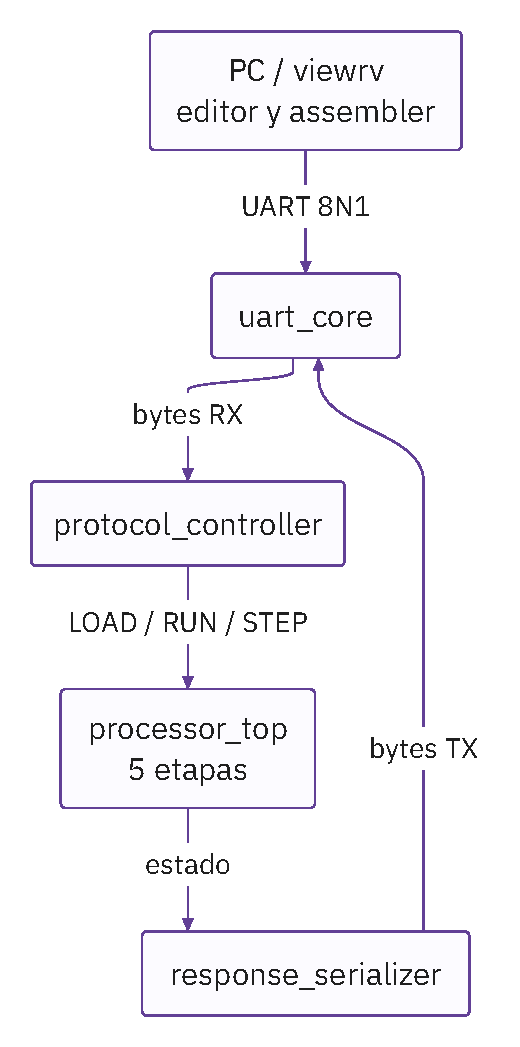
\includegraphics[width=0.34\textwidth]{sistema-general.pdf}
  \caption{Topología del sistema.}
  \label{fig:sistema-general}
\end{figure}

\section{Jerarquía y responsabilidades}

La jerarquía aprobada se resume en la tabla~\ref{tab:jerarquia}. El
inventario completo, con los 51 bloques del CPU y su ubicación, se
consulta en \doc{architecture/module_inventory.md}{Inventario de módulos}.

\begin{table}[H]
  \centering
  \small
  \begin{tabularx}{\textwidth}{L{4.8cm}Y}
    \toprule
    \textbf{Módulo} & \textbf{Responsabilidad} \\
    \midrule
    \code{basys3_top} & Adapta el sistema a la Basys 3: expone los cuatro
    puertos físicos, selecciona el perfil \code{MEMORY_PROFILE},
    instancia el Clocking
    Wizard (MMCM/BUFG de 100 a 50 MHz con \code{locked}), distribuye el
    \code{reset_sync} común y conecta \code{system_top}. \\ \addlinespace
    \code{system_top} & Integra el sistema funcional: conecta
    \code{uart_core}, \code{protocol_controller},
    \code{response_serializer} y \code{processor_top}, y distribuye clock,
    reset, capacidades de memoria y señales de observación. \\ \addlinespace
    \code{processor_top} & Contiene el procesador y sus servicios: pipeline de
    cinco etapas, cuatro registros interetapa, RF, IMEM/DMEM, forwarding y
    hazards, \code{execution_control}, \code{loader} y
    \code{session_preparation}; expone PC, RF, latches, fault y memoria
    utilizada para Debug. \\ \addlinespace
    \code{uart_core} & Implementa el transporte serie: sincroniza RX, genera
    el tick de sobremuestreo 16$\times$ para RX/TX, recibe y valida tramas
    8N1, transmite bytes y conserva FIFO independientes de cuatro bytes para
    recepción y transmisión. \\ \addlinespace
    \code{protocol_controller} & Interpreta \code{LOAD}, \code{RUN},
    \code{STEP}, \code{RESET} y \code{CHECK_READY}; valida tamaño y secuencia,
    coordina carga y preparación, solicita \code{RUN}/\code{STEP}, administra
    Debug, timeouts, silencio y recuperación. \\ \addlinespace
    \code{response_serializer} & Captura el descriptor del controlador y
    produce la respuesta completa: cabecera, contexto, banco de registros,
    latches y lista de DMEM. Lee el estado retenido para el snapshot y señala
    el fin físico del mensaje, incluido el último Stop. \\
    \bottomrule
  \end{tabularx}
  \caption{Jerarquía principal y responsabilidades.}
  \label{tab:jerarquia}
\end{table}

El CPU se distribuye en 51 bloques funcionales: 23 se implementan
como módulos específicos y 28 como lógica o estado local dentro de
una etapa o del top.

\section{Organización del procesador}

El procesador es un pipeline \emph{in-order} de cinco etapas. Cada instrucción
avanza como máximo una etapa por ciclo efectivo. La figura~\ref{fig:pipeline}
muestra el recorrido y la tabla~\ref{tab:etapas} resume la función de cada
etapa.

\begin{figure}[H]
  \centering
  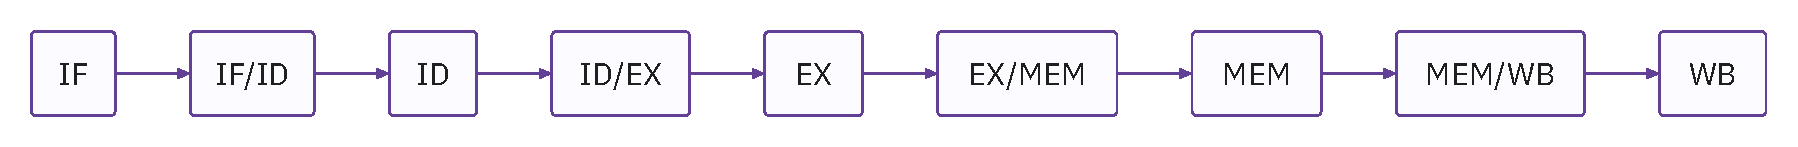
\includegraphics[width=\textwidth]{pipeline.pdf}
  \caption{Etapas y registros interetapa del procesador.}
  \label{fig:pipeline}
\end{figure}

\begin{table}[H]
  \centering
  \small
  \begin{tabularx}{\textwidth}{L{1.4cm}Y}
    \toprule
    \textbf{Etapa} & \textbf{Función principal} \\
    \midrule
    IF & Mantiene el PC, lee IMEM, valida la búsqueda y forma el candidato de
    fault de fetch. \\ \addlinespace
    ID & Decodifica la instrucción, lee el banco de registros, genera el
    inmediato, aplica el bypass \tech{WB}$\rightarrow$\tech{ID} y detecta
    load-use e instrucciones ilegales. \\ \addlinespace
    EX & Selecciona operandos con forwarding, ejecuta la ALU, calcula
    direcciones, resuelve branches y jumps, y confirma faults propios y
    la instrucción \code{halt}. \\ \addlinespace
    MEM & Accede a DMEM, selecciona y extiende loads, aplica la máscara de
    stores y forma el valor de writeback. \\ \addlinespace
    WB & Escribe el banco de registros y genera los controles de bypass hacia
    ID. \\
    \bottomrule
  \end{tabularx}
  \caption{Responsabilidad de cada etapa.}
  \label{tab:etapas}
\end{table}

Los cuatro registros interetapa conservan la validez y los campos que la etapa
siguiente necesita; su organización y la semántica de validez se detallan en la
sección~\ref{sec:registros-interetapa}.

\section{Conjunto de instrucciones}

El decoder implementa 32 instrucciones de \tech{RV32I} y la palabra exacta de
\code{halt}. A continuación se resumen las familias de instrucciones.

\begin{table}[H]
  \centering
  \small
  \begin{tabularx}{\textwidth}{L{3.2cm}Y}
    \toprule
    \textbf{Familia} & \textbf{Instrucciones} \\
    \midrule
    Registro & \code{ADD}, \code{SUB}, \code{SLL}, \code{SLT}, \code{SLTU},
    \code{XOR}, \code{SRL}, \code{SRA}, \code{OR}, \code{AND} \\
    \addlinespace
    Inmediato & \code{ADDI}, \code{SLTI}, \code{SLTIU}, \code{XORI},
    \code{ORI}, \code{ANDI}, \code{SLLI}, \code{SRLI}, \code{SRAI} \\
    \addlinespace
    Loads & \code{LB}, \code{LH}, \code{LW}, \code{LBU}, \code{LHU} \\
    \addlinespace
    Stores & \code{SB}, \code{SH}, \code{SW} \\
    \addlinespace
    Flujo & \code{BEQ}, \code{BNE}, \code{JAL}, \code{JALR} \\
    \addlinespace
    Inmediato superior & \code{LUI} \\
    \addlinespace
    Terminación & \code{halt} = \code{0x0000000B} \\
    \bottomrule
  \end{tabularx}
  \caption{Subconjunto de instrucciones implementado.}
  \label{tab:isa}
\end{table}

\code{halt} se codifica con la palabra exacta \code{0x0000000B}. Los bits
31:7 son cero y los bits 6:0 forman el opcode \code{0001011}, que el mapa de
RISC-V User-Level ISA V2.2 reserva para la extensión \code{custom-0}. La
instrucción no tiene operandos y no escribe el banco de registros ni DMEM.

La codificación se adoptó para disponer de una terminación explícita sin
reutilizar una instrucción estándar con otra semántica. Usar \code{EBREAK}
habría mezclado la finalización normal con una excepción de breakpoint, y
reservar \code{0x00000000} habría confundido una memoria sin programar con un
\code{halt} intencional. El espacio \code{custom-0} permite introducir la
instrucción sin colisionar con RV32I, y la palabra completa distingue
\code{halt} de cualquier otra codificación custom.

Toda instrucción distinta de las codificaciones admitidas produce
\code{ILLEGAL_INSTRUCTION}. La legalidad se comprueba en ID; la memoria no
decide si una palabra es una instrucción válida.

\section{Separación entre datos y control}

El camino de datos o \emph{datapath} reúne los bloques que almacenan y
procesan la información: el PC, el banco de registros, las memorias, la ALU,
los sumadores y los multiplexores. Por estos bloques circulan las
instrucciones, sus operandos y los resultados. Las señales de control indican
qué operación realizar, qué entrada elegir en cada multiplexor y cuándo
actualizar el PC y los registros interetapa.

El control se distribuye entre los siguientes bloques:

\begin{itemize}
  \item \textbf{Decoder:} identifica la operación que solicita cada instrucción
  y genera sus señales de control.
  \item \textbf{Unidad de forwarding:} selecciona resultados de instrucciones
  anteriores para que EX pueda utilizarlos antes de que se escriban en el
  banco de registros.
  \item \textbf{Detector de \code{load-use}:} identifica cuándo una instrucción
  debe esperar porque necesita el dato de un load que aún no está disponible.
  \item \textbf{\code{Flow Control}:} determina si corresponde cambiar el flujo
  de ejecución y selecciona qué dirección de destino utilizar.
  \item \textbf{Comprobadores de fault:} detectan errores en las instrucciones
  y en los accesos a memoria.
  \item \textbf{\code{Pipeline Hazard Control}:} reúne esas condiciones y
  decide qué instrucciones pueden continuar, cuáles deben esperar y cuáles
  se deben descartar.
\end{itemize}

En cada ciclo habilitado por \code{cpu_cycle_fire},
\code{Pipeline Hazard Control} elige una sola acción. Fuera del modo de
drenado, aplica la primera condición que se cumpla en este orden:

\begin{enumerate}
  \item Fault de la instrucción en EX.
  \item \code{halt} en EX.
  \item Cambio de flujo resuelto en EX.
  \item Fault de la instrucción en ID.
  \item Espera por una dependencia \code{load-use}.
  \item Avance normal, si no se cumple ninguna de las condiciones anteriores.
\end{enumerate}

Los eventos de EX tienen prioridad sobre los de ID porque corresponden a una
instrucción anterior en el programa. Además, un fault de la propia instrucción
impide aplicar sus otros efectos.

Durante el drenado (\code{drain_mode}), el control deja de incorporar
instrucciones nuevas y permite que terminen las que siguen activas. Para este
modo hay dos acciones adicionales: avanzar o esperar por una dependencia
\code{load-use}. En total se definen ocho acciones, cuyos efectos sobre el PC
y los registros interetapa se detallan en la tabla~\ref{tab:acciones} y en
\doc{architecture/cpu/control_and_hazards.md}{Control y hazards}. Si
\code{cpu_cycle_fire} vale cero, no se aplica ninguna de ellas.

\section{Debug y observación}

Debug permite consultar el estado que la ejecución ya dejó registrado, sin
modificarlo ni agregar ciclos al procesador. La observación combina dos tipos
de información:

\begin{itemize}
  \item \textbf{Estado arquitectónico:} PC, contador de ciclos, causa y PC de
  fault, banco de registros y bytes de DMEM que fueron utilizados.
  \item \textbf{Estado del pipeline:} validez y contenido de los registros
  \code{IF/ID}, \code{ID/EX}, \code{EX/MEM} y \code{MEM/WB}. Estos registros
  permiten saber qué instrucciones todavía están en vuelo y qué datos llevan
  entre etapas.
\end{itemize}

El controlador de protocolo retiene la CPU mientras se arma la respuesta. En
ese intervalo selecciona, de manera alternada, las direcciones de lectura del
banco de registros y de DMEM. El serializador toma esas lecturas y los campos
de los registros interetapa, y los transmite en el orden fijado por el
protocolo. Así, todos los campos del snapshot corresponden al mismo estado
observado.

El snapshot contiene:

\begin{itemize}
  \item el estado global de la sesión y la validez de la imagen cargada;
  \item el PC y el contador de ciclos;
  \item la causa y el PC del fault, cuando existe;
  \item los 32 registros del banco de registros;
  \item los campos definidos de los cuatro registros interetapa;
  \item la cantidad de bytes utilizados de DMEM y la lista de sus direcciones
  y valores.
\end{itemize}

La observación se realiza después del último ciclo autorizado, por ejemplo,
después de un \code{STEP} o al finalizar un \code{RUN}.

La estructura y los códigos se detallan en \doc{protocol.md}{Protocolo UART} y en
\doc{architecture/debug/debug_architecture.md}{Arquitectura de Debug}.


\chapter{Procesador RISC-V de cinco etapas}\label{chap:procesador}
\section{Organización general}

El procesador implementa un pipeline \emph{in-order} de cinco etapas. La
arquitectura mantiene el orden del programa: una instrucción más nueva no puede
adelantarse a una anterior ni modificar el estado arquitectónico antes que
ella. El solapamiento cambia cuántas instrucciones están activas al mismo
tiempo, pero no la semántica secuencial.

El recorrido de las cinco etapas se muestra en la
figura~\ref{fig:pipeline}. Las etapas y sus contratos se desarrollan en
\doc{architecture/cpu/cpu_pipeline.md}{Pipeline de la CPU}; el detalle de
señales, muxes y caminos de datos se encuentra en
\doc{architecture/cpu/datapath.md}{Datapath}.

\section{Modelo temporal y ocupación}

En un ciclo efectivo, cada etapa trabaja sobre una instrucción distinta y los
registros interetapa capturan el resultado de la etapa anterior. La
tabla~\ref{tab:ocupacion} muestra la ocupación ideal de cinco instrucciones
independientes, sin hazards ni cambios de flujo. Cada instrucción avanza una
etapa por ciclo y el pipeline alcanza a tener cinco instrucciones activas.

\begin{table}[H]
  \centering
  \small
  \setlength{\tabcolsep}{3pt}
  \begin{tabular}{l*{9}{c}}
    \toprule
    \textbf{Instrucción} & C1 & C2 & C3 & C4 & C5 & C6 & C7 & C8 & C9 \\
    \midrule
    I1 & IF & ID & EX & MEM & WB & --- & --- & --- & --- \\
    I2 & --- & IF & ID & EX & MEM & WB & --- & --- & --- \\
    I3 & --- & --- & IF & ID & EX & MEM & WB & --- & --- \\
    I4 & --- & --- & --- & IF & ID & EX & MEM & WB & --- \\
    I5 & --- & --- & --- & --- & IF & ID & EX & MEM & WB \\
    \bottomrule
  \end{tabular}
  \caption{Ocupación ideal de cinco instrucciones independientes. Cada columna
  representa un ciclo efectivo y cada fila una instrucción.}
  \label{tab:ocupacion}
\end{table}

En el régimen ideal, el pipeline entrega una instrucción por ciclo después de
llenarse, por lo que el CPI se aproxima a uno. Las desviaciones tienen causas
concretas:

\begin{itemize}
  \item Una dependencia inmediata \code{load-use} retiene al consumidor e
    inserta una burbuja en \code{ID/EX}. El load avanza y el consumidor
    continúa un ciclo después, cuando el dato ya puede reenviarse a traves de forwarding.
  \item Un branch tomado, \code{JAL} o \code{JALR} se resuelve en EX. El
    redirect invalida las dos instrucciones más jóvenes que ya habían entrado
    al pipeline y produce una penalización de dos ciclos.
  \item Un fault confirmado o un \code{halt} detiene el ingreso de instrucciones
    nuevas. El pipeline se drena para completar solamente las instrucciones
    anteriores que todavía estaban en vuelo.
\end{itemize}

\section{Instruction Fetch (IF)}

La etapa IF inicia el recorrido de cada instrucción. En cada ciclo efectivo
consulta la dirección indicada por el PC global, obtiene una palabra de IMEM y
forma el candidato que el control puede capturar en \code{IF/ID}. La lectura de IMEM es
combinacional: la palabra está disponible dentro del mismo ciclo.

En el recorrido secuencial, IF propone \code{PC + 4} como próximo PC. Si EX
confirma un branch tomado, \code{JAL} o \code{JALR}, el control reemplaza esa
dirección por el destino del redirect y descarta las instrucciones jóvenes que
ya habían sido buscadas.

Los bloques principales de la etapa son:

\begin{itemize}
  \item \textbf{\code{PC}:} conserva la dirección de la búsqueda actual y se
    actualiza cuando el control habilita un nuevo ciclo de ejecución.
  \item \textbf{\code{PC Adder}:} calcula la continuación secuencial sumando
    cuatro bytes al PC actual.
  \item \textbf{\code{Next PC MUX}:} selecciona entre \code{PC + 4} y el
    destino de un redirect producido por EX.
  \item \textbf{\code{PC Update Control}:} determina si el PC debe actualizarse
    y qué entrada del multiplexor debe utilizarse.
  \item \textbf{\code{Instruction Memory}:} entrega la palabra de 32 bits
    almacenada en la dirección indicada por el PC.
  \item \textbf{\code{Fetch Fault Check}:} comprueba la alineación, el rango
    de IMEM y la pertenencia de los cuatro bytes a la imagen cargada.
  \item \textbf{\code{IF/ID Input Logic}:} combina la instrucción, su PC y el
    resultado de la validación para formar los campos de entrada de \code{IF/ID}.
  \item \textbf{\code{IF/ID Update Control}:} traduce la acción del pipeline en
    una captura, una retención o una invalidación del registro interetapa.
  \item \textbf{Registro \code{IF/ID}:} conserva la instrucción o el candidato
    de fault de fetch hasta que ID pueda procesarlo.
\end{itemize}

Antes de aceptar el resultado como instrucción, IF valida la búsqueda:

\begin{itemize}
  \item el PC debe estar alineado a cuatro bytes;
  \item los cuatro bytes deben pertenecer a la capacidad de IMEM;
  \item los cuatro bytes deben pertenecer a la imagen confirmada.
\end{itemize}

Si la validación falla, IF no produce una instrucción activa: genera un
\emph{candidato de fault de fetch}. El candidato conserva el PC y la causa, y
se transporta por \code{IF/ID}. La confirmación arquitectónica ocurre en ID,
después de respetar el orden de las instrucciones anteriores. Este mecanismo se
describe en \doc{architecture/session/faults_and_termination.md}{Faults,
redirects y terminación}.

El registro \code{IF/ID} conserva cinco campos: \code{valid}, \code{pc},
\code{instruction}, \code{fetch_fault_valid} y
\code{fetch_fault_cause}. En un estado legal, \code{valid} y
\code{fetch_fault_valid} no están activos simultáneamente. La
figura~\ref{fig:etapa-if} muestra el recorrido completo de la etapa.

\begin{figure}[H]
  \centering
  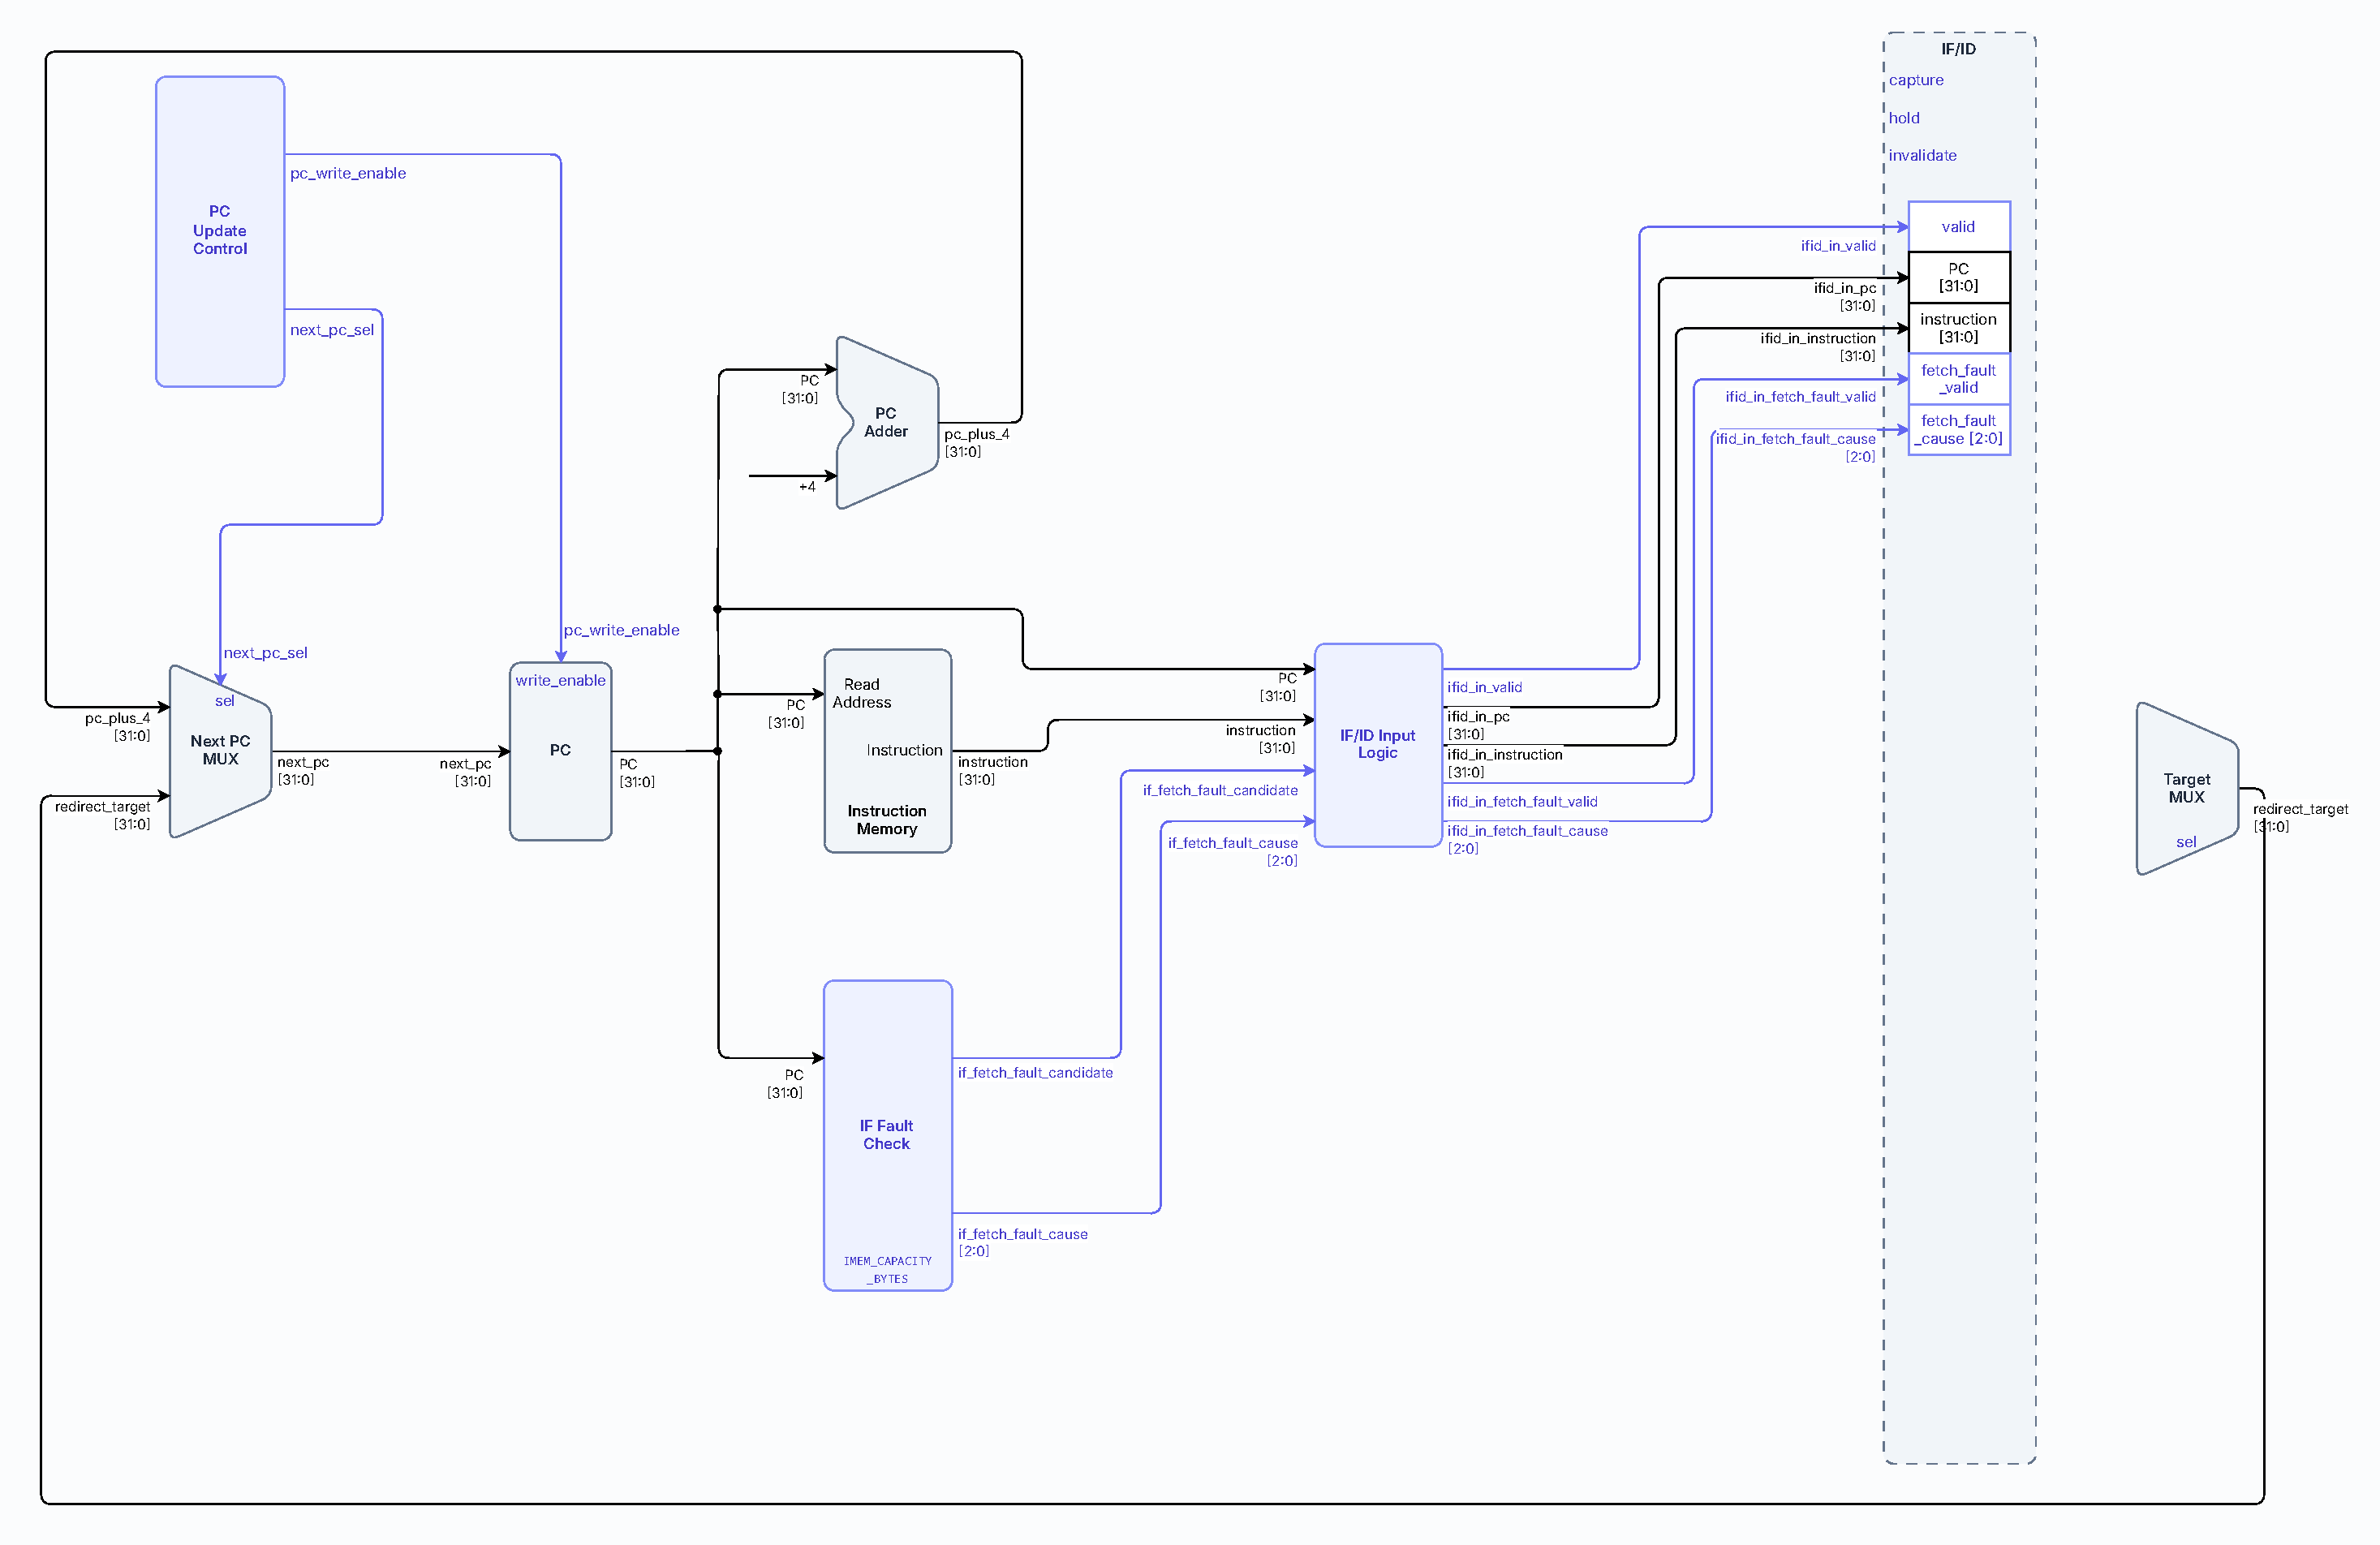
\includegraphics[width=0.95\textwidth]{if-normal.pdf}
  \caption{Recorrido de IF: PC, adder, Instruction Memory, comprobador de
  fetch e IF/ID.}
  \label{fig:etapa-if}
\end{figure}

\section{Instruction Decode (ID)}

La etapa ID recibe desde \code{IF/ID} la instrucción y su PC. En paralelo,
comprueba si la codificación es válida, obtiene los operandos, genera el
inmediato y prepara las señales que EX, MEM y WB necesitarán más adelante.
También resuelve las dependencias que pueden detectarse en esta etapa. El
resultado de ese procesamiento se captura en \code{ID/EX} solo cuando la
acción del pipeline permite avanzar.

\subsection{Bloques principales}

Sus bloques principales son:

\begin{itemize}
  \item \textbf{\code{Decoder}:} reconoce las instrucciones de la whitelist y
    genera los controles de ALU, memoria, flujo, selección de resultado y
    escritura.
  \item \textbf{\code{Register File}:} proporciona las dos lecturas de los
    registros fuente y recibe la escritura síncrona de WB; \code{x0} conserva
    siempre el valor cero.
  \item \textbf{\code{Immediate Generator}:} reconstruye y extiende el
    inmediato según el formato I, S, B, U o J de la instrucción.
  \item \textbf{\code{WB Bypass Control}:} detecta si WB escribe efectivamente
    uno de los registros que ID está leyendo en el mismo ciclo.
  \item \textbf{\code{RS1 Bypass MUX}:} selecciona el valor de WB para la
    fuente \code{rs1} cuando hay coincidencia; si no, conserva la lectura del
    banco de registros.
  \item \textbf{\code{RS2 Bypass MUX}:} aplica la misma selección a la fuente
    \code{rs2}, de manera independiente.
  \item \textbf{\code{ID Fault Check}:} combina una codificación ilegal con un
    candidato de fault de fetch para producir el candidato de fault de ID.
  \item \textbf{\code{Load-Use Detector}:} compara el destino de un load en
    \code{ID/EX} con las fuentes que consume la instrucción de \code{IF/ID} y
    solicita una espera cuando la dependencia es inmediata.
  \item \textbf{\code{ID/EX Update Control}:} convierte la acción del pipeline
    en una captura de ID, una retención o una burbuja.
  \item \textbf{Registro \code{ID/EX}:} conserva los operandos, el inmediato,
    el PC y los controles que EX necesita para ejecutar la instrucción.
\end{itemize}

Una vez decodificada la instrucción y aplicados los bypass, ID prepara la
entrada de \code{ID/EX}. Allí quedan registrados los operandos que EX debe
utilizar, el inmediato, el PC, el registro destino y los controles que indican
qué operación realizar, si hay un acceso a memoria y si habrá una escritura en
WB.

Además, ID determina si la instrucción usa realmente \code{rs1} o \code{rs2}.
Esas dos señales (\code{uses_rs1} y \code{uses_rs2}) sirven para que EX y el detector de
\code{load-use} comparen solo las fuentes relevantes. Como se pueden obtener
directamente de la palabra de instrucción, se mantienen como señales
combinacionales y no se almacenan como campos adicionales en \code{ID/EX}.

El banco de registros tiene dos puertos de lectura combinacional y una escritura
síncrona. La escritura solo es efectiva si el ciclo está habilitado, la entrada
de \code{MEM/WB} es válida, \code{reg_write} está activo y el destino no es
\code{x0}. Si ID lee ese mismo registro en el ciclo de writeback, los muxes de
bypass seleccionan directamente el valor de \code{MEM/WB}; así, la captura en
\code{ID/EX} no depende de la semántica de lectura y escritura simultáneas del
almacenamiento físico. La figura~\ref{fig:etapa-id} resume los bloques y caminos
de la etapa.

\begin{figure}[H]
  \centering
  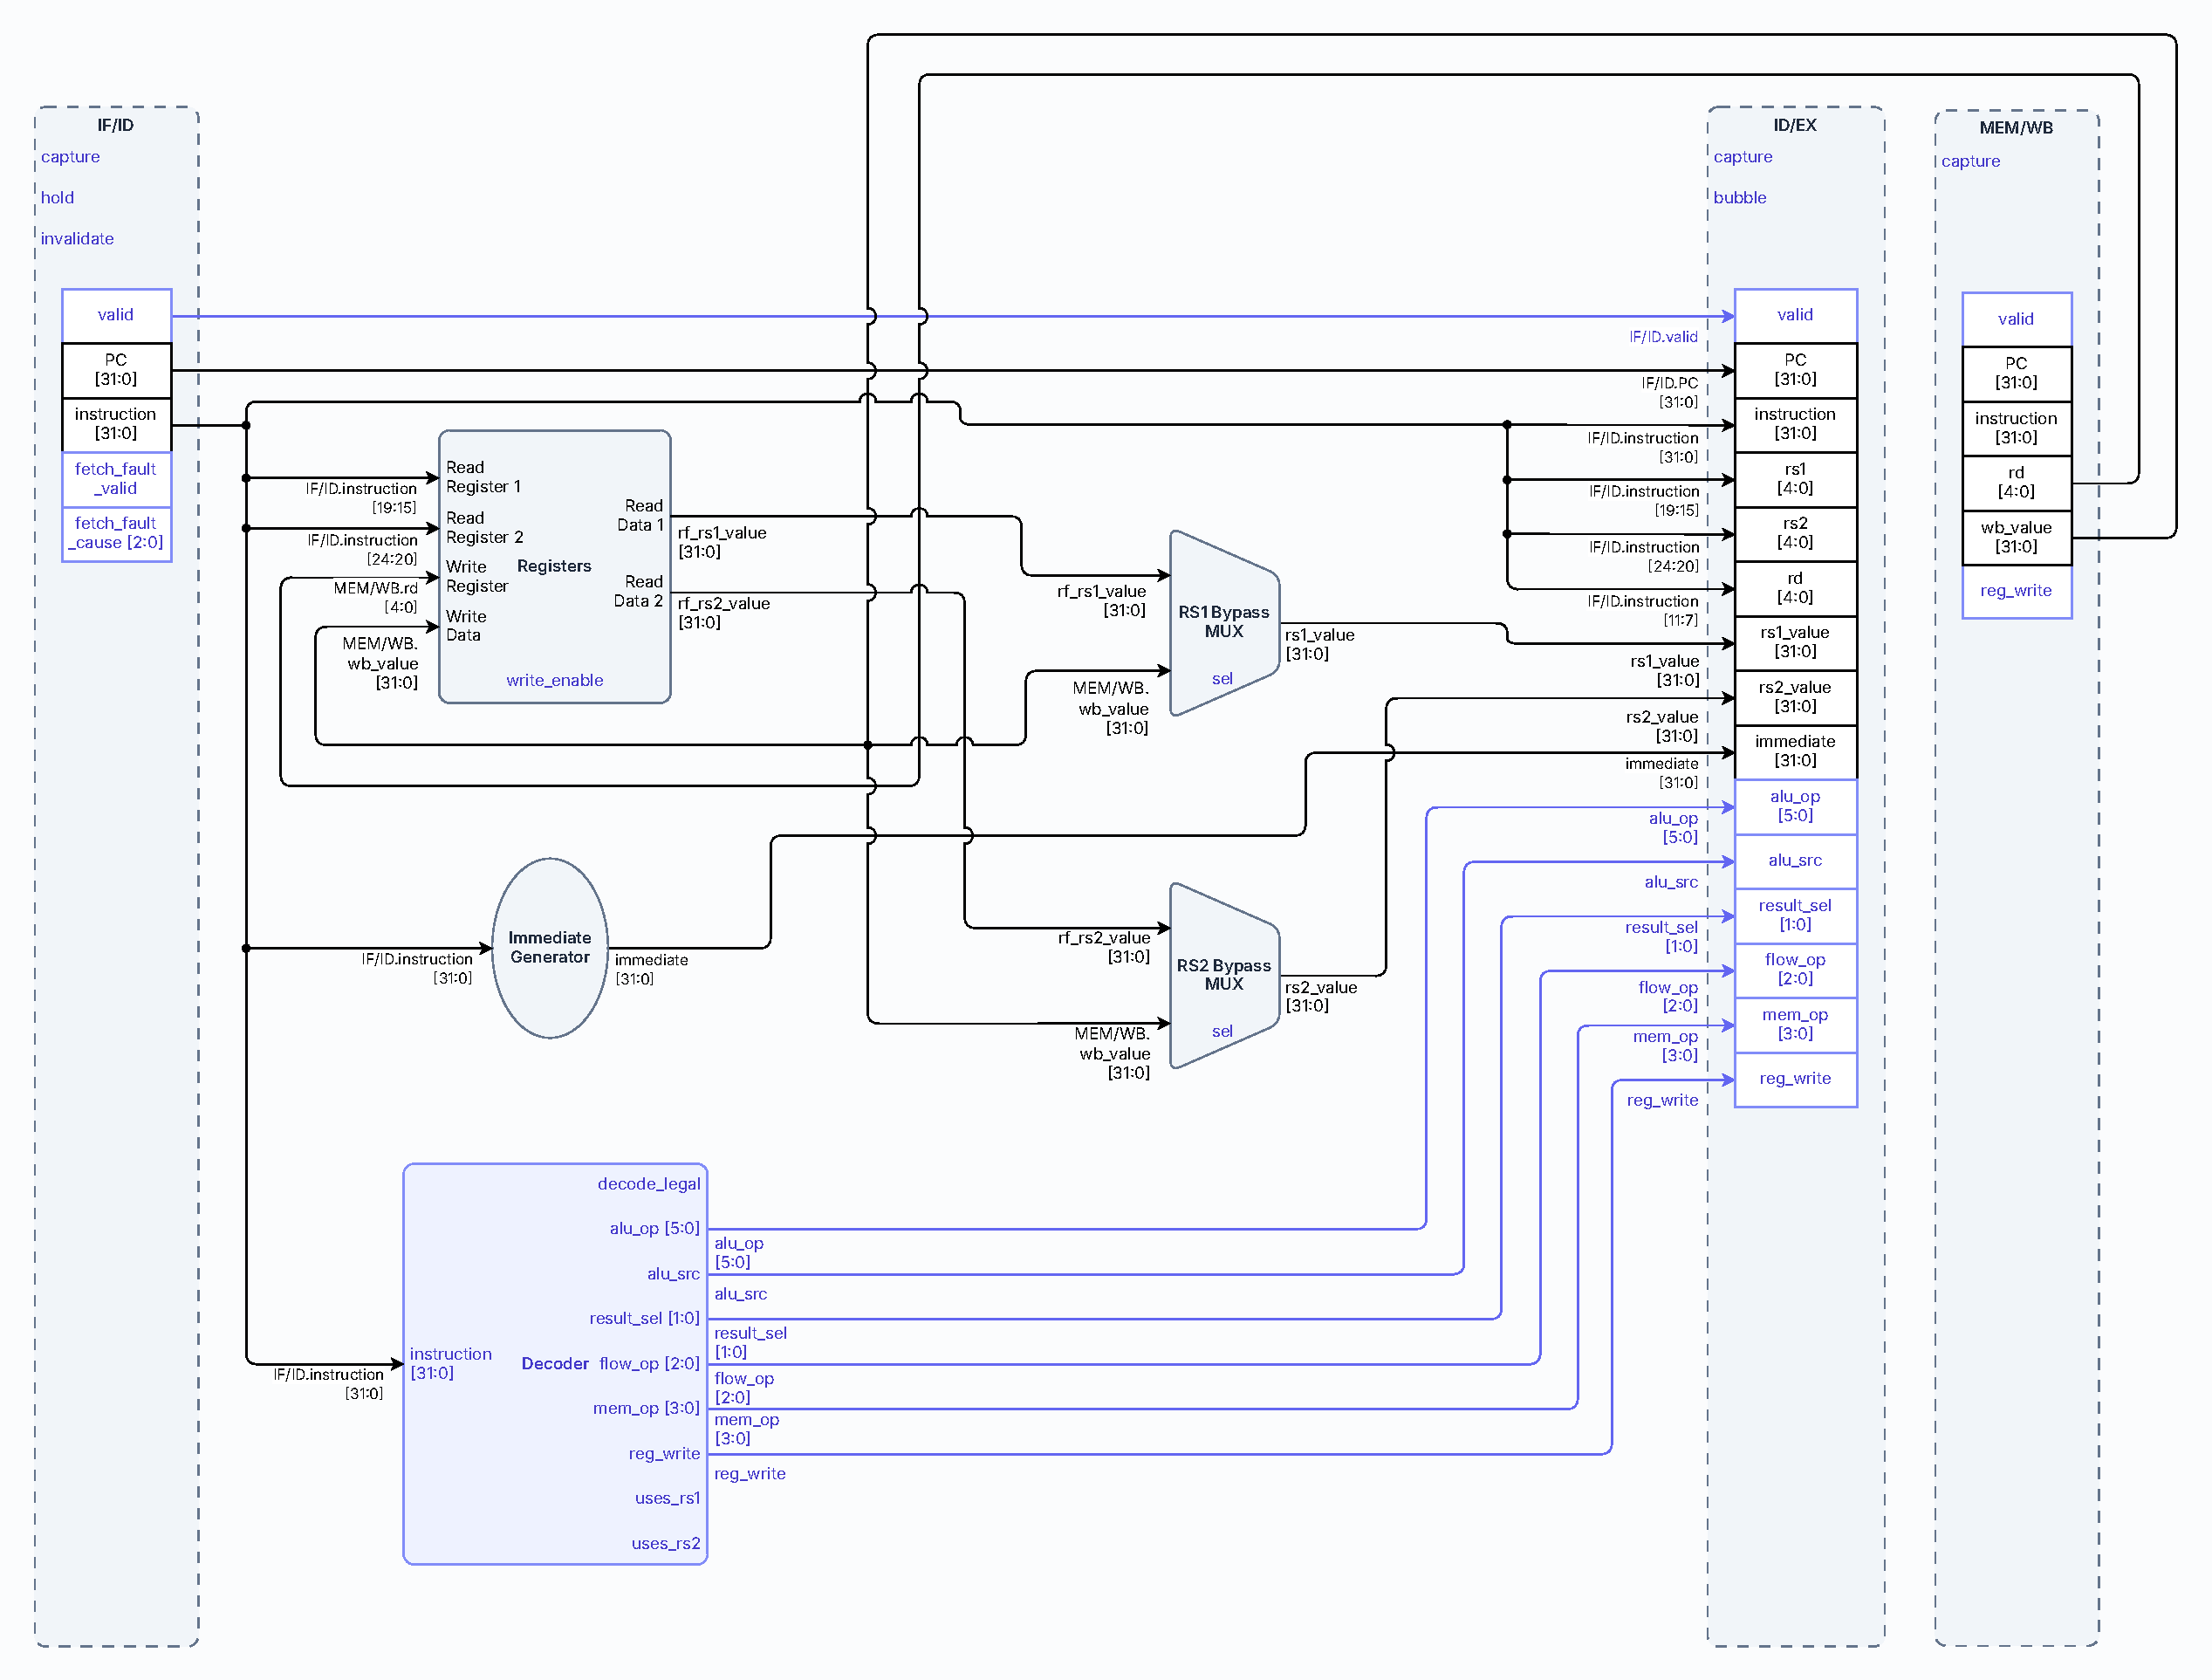
\includegraphics[width=0.95\textwidth]{id-normal.pdf}
  \caption{Recorrido de ID: decoder, banco de registros, generador de
  inmediatos, comprobación de fault y bypass WB$\rightarrow$ID.}
  \label{fig:etapa-id}
\end{figure}

\subsection{Señales de control de ID}

Como resultado de la decodificación, el \code{Decoder} traduce la palabra de
instrucción en un conjunto acotado de señales.
La tabla~\ref{tab:senales-control} resume los códigos que atraviesan
\code{ID/EX} y que después consumen EX, MEM y WB. Los campos
\code{uses_rs1} y \code{uses_rs2} no se almacenan: se calculan a partir de la
instrucción para el forwarding y el detector de load-use.

\begin{table}[H]
  \centering
  \footnotesize
  \setlength{\tabcolsep}{3pt}
  \begin{tabularx}{\textwidth}{L{2.4cm}L{1.0cm}Y}
    \toprule
    \textbf{Señal} & \textbf{Ancho} & \textbf{Valores y significado} \\
    \midrule
    \code{alu_op} & 6 & \code{SLL=0x00}, \code{SRL=0x02}, \code{SRA=0x03},
    \code{ADD=0x20}, \code{SUB=0x22}, \code{AND=0x24}, \code{OR=0x25},
    \code{XOR=0x26}, \code{SLT=0x2A}, \code{SLTU=0x2B}. \\
    \addlinespace
    \code{alu_src} & 1 & \code{0}: segundo operando desde \code{rs2};
    \code{1}: desde el inmediato. \\
    \addlinespace
    \code{result_sel} & 2 & \code{0}: resultado de ALU; \code{1}: inmediato;
    \code{2}: enlace de \code{JAL}/\code{JALR}. \\
    \addlinespace
    \code{flow_op} & 3 & \code{NONE=0}, \code{BEQ=1}, \code{BNE=2},
    \code{JAL=3}, \code{JALR=4}, \code{HALT=5}. \\
    \addlinespace
    \code{mem_op} & 4 & \code{NONE=0}, \code{LB=1}, \code{LH=2}, \code{LW=3},
    \code{LBU=4}, \code{LHU=5}, \code{SB=6}, \code{SH=7}, \code{SW=8}. \\
    \addlinespace
    \code{reg_write} & 1 & \code{0}: no escribe RF; \code{1}: escribe el
    registro \code{rd} si es válido y distinto de \code{x0}. \\
    \bottomrule
  \end{tabularx}
  \caption{Señales de control producidas por el decoder.}
  \label{tab:senales-control}
\end{table}

\section{Execute (EX)}

EX recibe desde \code{ID/EX} una instrucción decodificada, sus operandos base,
el inmediato y las señales de control. Es una etapa combinacional: durante el mismo
ciclo resuelve los operandos, calcula resultados y direcciones, forma los
destinos de salto y genera los candidatos de redirect, \code{halt} y fault.

Sus bloques principales son:

\begin{itemize}
  \item \textbf{\code{Forwarding Unit}:} identifica los productores más
    recientes y selecciona qué valor debe utilizar cada fuente.
  \item \textbf{\code{Forward MUX A} y \code{Forward MUX B}:} producen los
    operandos efectivos \code{rs1_effective} y \code{rs2_effective}.
  \item \textbf{\code{ALU Source MUX}:} elige entre \code{rs2_effective} y el
    inmediato para el segundo operando de la ALU.
  \item \textbf{\code{ALU}:} ejecuta operaciones aritméticas, lógicas,
    comparaciones y desplazamientos, y calcula direcciones efectivas.
  \item \textbf{\code{Link Adder}:} calcula \code{PC + 4}, el valor de enlace
    de \code{JAL} y \code{JALR}.
  \item \textbf{\code{Result MUX}:} selecciona el resultado de ALU, el
    inmediato o el enlace que se conservará como \code{ex_result}.
  \item \textbf{\code{Target Adder} y \code{JALR Adder}:} forman,
    respectivamente, los destinos relativos al PC y los destinos basados en
    \code{rs1}.
  \item \textbf{\code{Clear bit 0} y \code{Target MUX}:} ajustan y seleccionan
    el destino final de un cambio de flujo.
  \item \textbf{\code{Flow Control}:} determina si un branch se toma y genera
    las solicitudes de redirect o el candidato de \code{halt}.
  \item \textbf{\code{EX Fault Check}:} valida accesos a DMEM y destinos de
    control, y produce el candidato de fault propio de EX.
  \item \textbf{\code{EX/MEM Update Control} y registro \code{EX/MEM}:}
    capturan los datos que MEM, WB y Debug todavía necesitan.
\end{itemize}

\subsection{Resolución de operandos}

La unidad de forwarding actúa antes de todos los usos de los operandos. Los
valores efectivos alimentan:

\begin{itemize}
  \item la ALU, para operaciones aritméticas, lógicas, comparaciones y
    desplazamientos;
  \item el cálculo de la dirección efectiva de loads y stores;
  \item la comparación de branches;
  \item la base de \code{JALR};
  \item el sumador de enlace y el cálculo de destinos de \code{JAL}.
\end{itemize}

La figura~\ref{fig:etapa-ex} resume el camino de una operación de registro.

\begin{figure}[H]
  \centering
  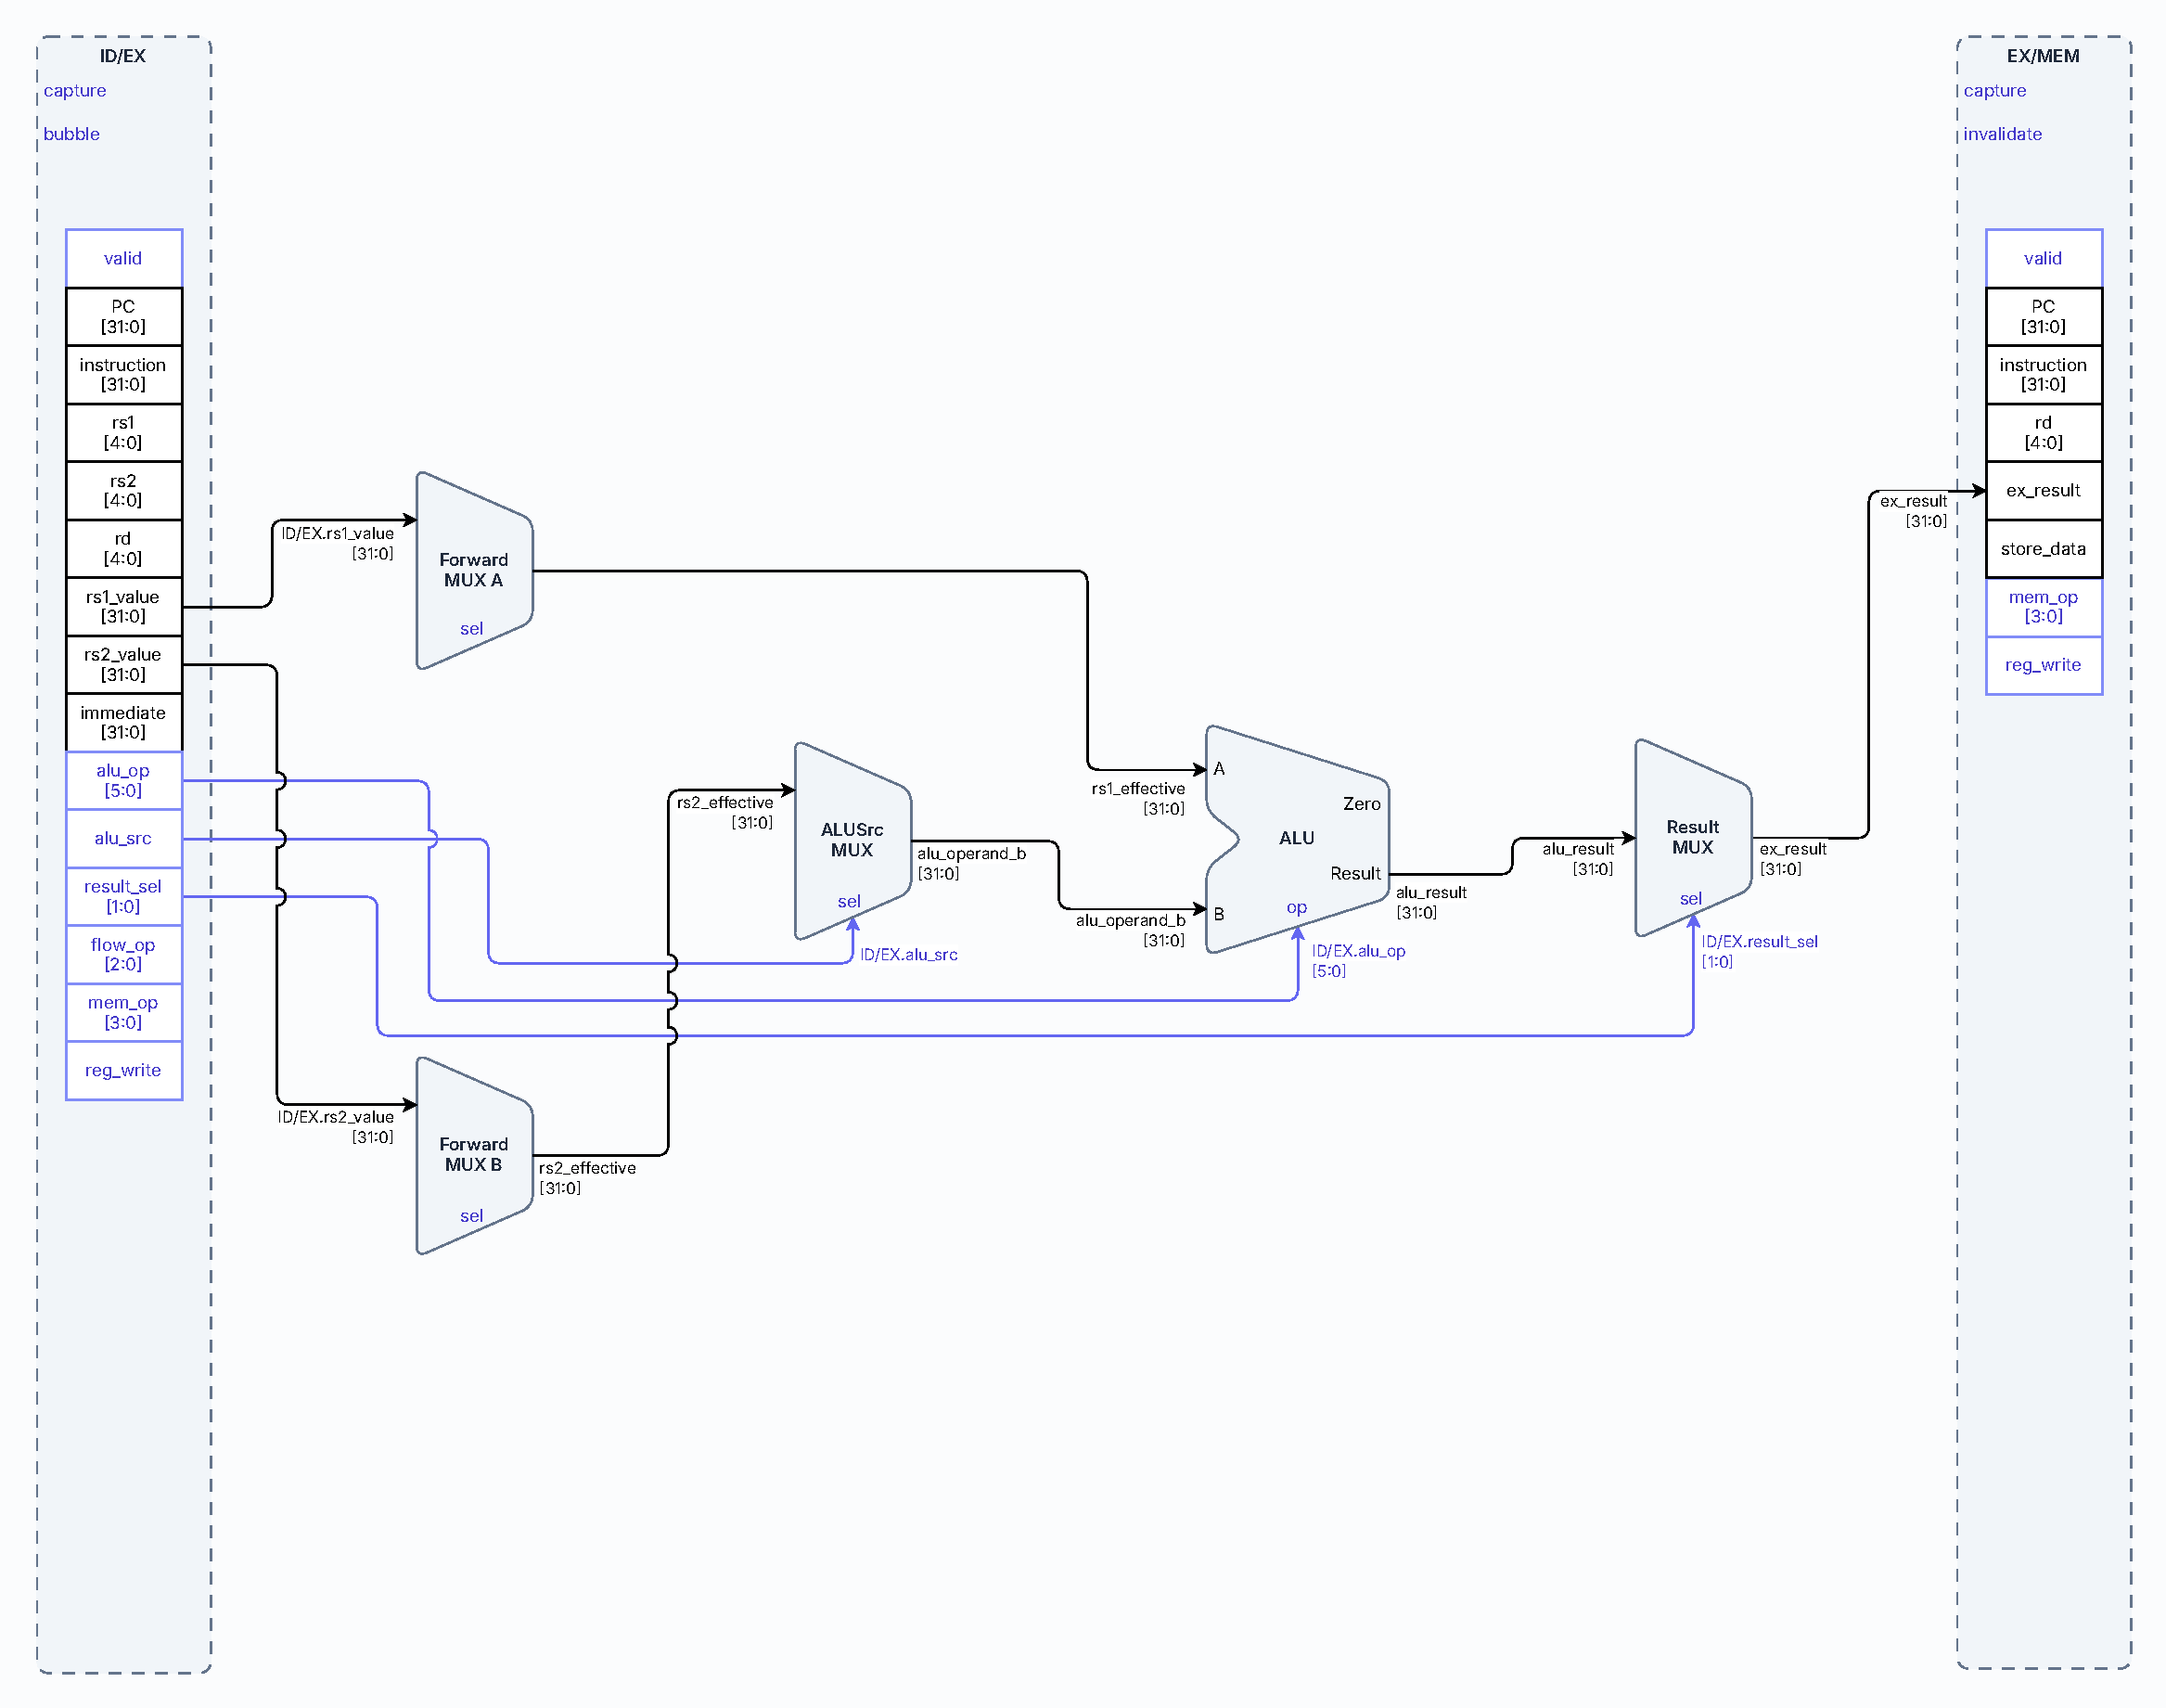
\includegraphics[width=0.92\textwidth]{ex-r.pdf}
  \caption{Recorrido de EX para una operación de registro: forwarding,
  ALU y selección del resultado.}
  \label{fig:etapa-ex}
\end{figure}

\subsection{Resultados y validaciones}

La ALU ejecuta la operación indicada por \code{alu_op}. Luego,
\code{result_sel} elige qué valor representa el resultado de la instrucción:
el resultado de la ALU, el inmediato o el enlace \code{PC + 4}. Para un load o
un store, ese resultado es la dirección efectiva; para \code{LUI} es el
inmediato y para \code{JAL}/\code{JALR} es el enlace. EX también valida la
alineación y el rango de los accesos a datos y de los destinos de control. Un
fault propio de EX tiene prioridad sobre el efecto normal de la misma
instrucción.

\begin{figure}[H]
  \centering
  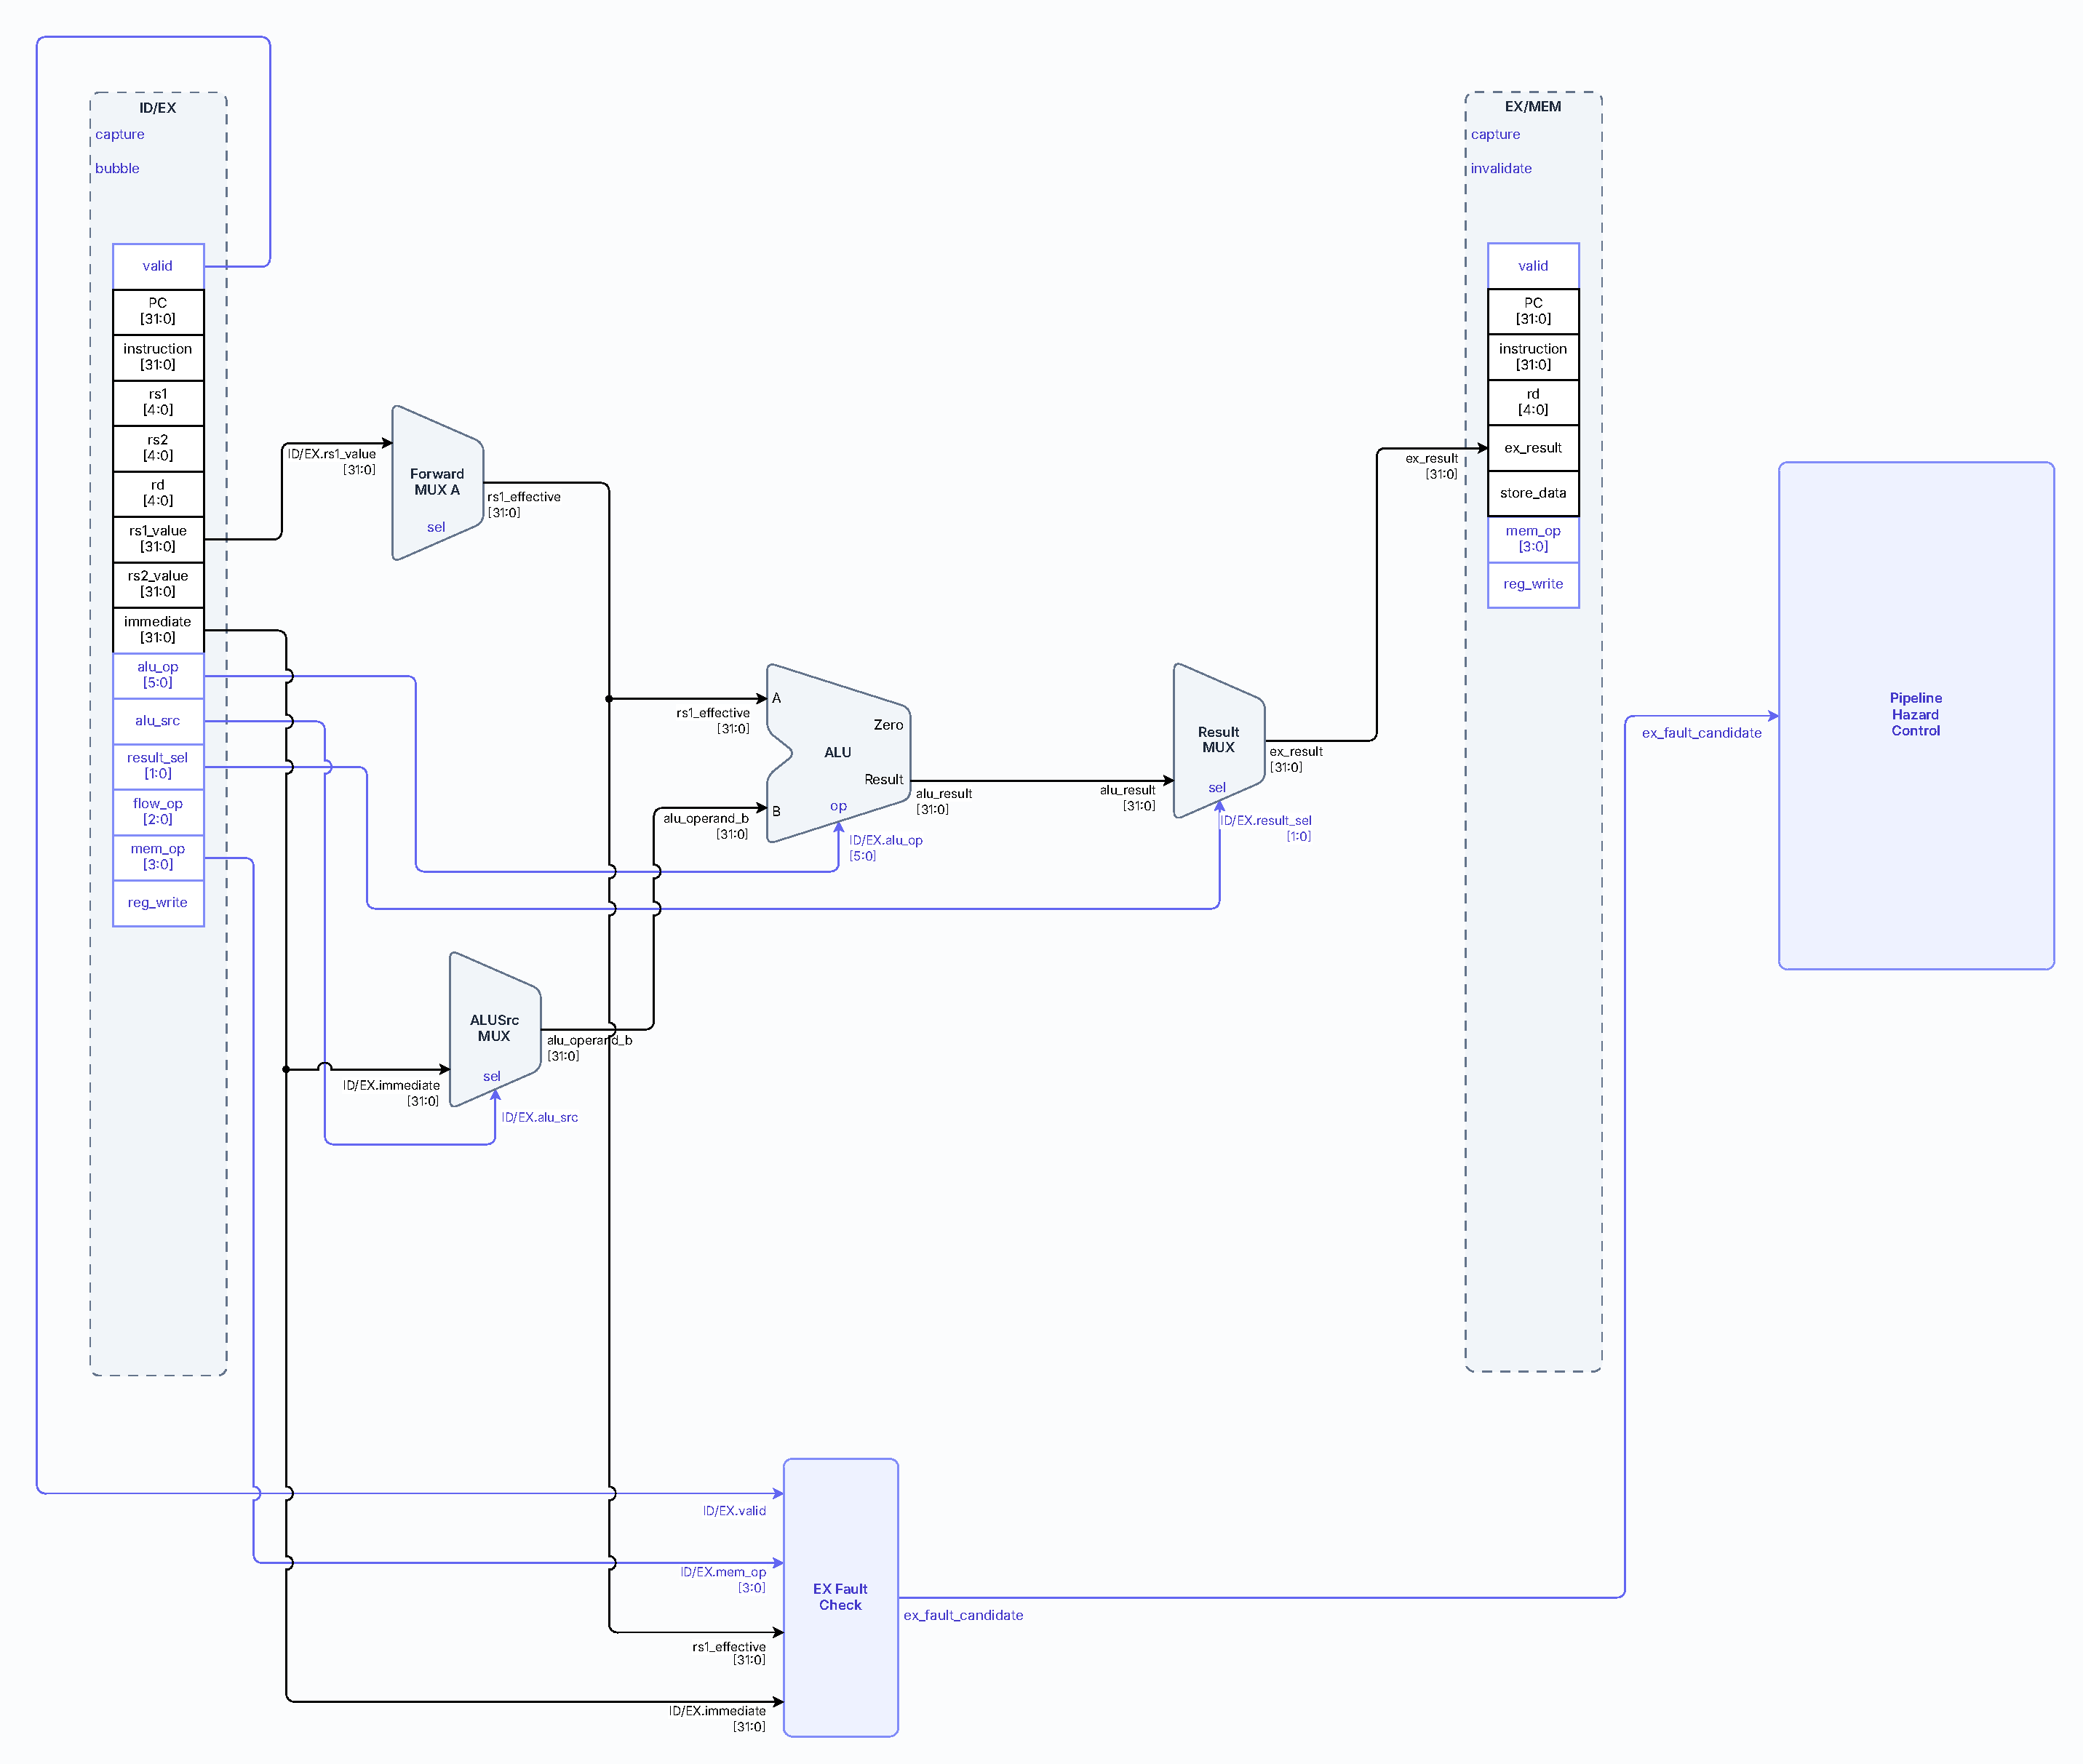
\includegraphics[width=0.80\textwidth]{ex-load.pdf}
  \caption{Recorrido de un load en EX: dirección efectiva, validación de
  alineación y rango, y preparación del acceso a MEM.}
  \label{fig:etapa-ex-load}
\end{figure}

\subsection{Cambios de flujo y terminación}

Los cambios de flujo se resuelven con los operandos efectivos:

\begin{itemize}
  \item \code{BEQ} toma el branch cuando ambos operandos son iguales y
    \code{BNE} cuando son distintos. Su destino, al igual que el de \code{JAL},
    es \code{ID/EX.pc + immediate}.
  \item \code{JALR} forma \code{(rs1_effective + immediate) \& 0xFFFFFFFE};
    después se comprueba que el destino esté alineado a cuatro bytes.
  \item \code{JAL} y \code{JALR} calculan además el enlace
    \code{ID/EX.pc + 4}, que se conserva para WB cuando no hay fault.
\end{itemize}

Cuando un branch tomado, \code{JAL} o \code{JALR} solicita un redirect, el
control actualiza el PC e invalida las instrucciones posteriores que ya habían
ingresado al pipeline. La instrucción de control sigue hacia \code{EX/MEM} para
conservar su enlace o completar su recorrido temporal. \code{halt}, en cambio,
se confirma en EX y no ingresa válidamente a \code{EX/MEM}; las instrucciones
anteriores todavía pueden completar durante el drenado.

\section{Memory (MEM)}

MEM recibe desde \code{EX/MEM} una instrucción cuya dirección efectiva ya fue
calculada y validada en EX. A partir de \code{mem_op}, determina si debe leer,
escribir o simplemente transportar el resultado de EX. La etapa es
combinacional entre \code{EX/MEM} y \code{MEM/WB}, salvo por la escritura
síncrona que realiza un store en el flanco del ciclo efectivo.

Sus bloques principales son:

\begin{itemize}
  \item \textbf{\code{MEM Decode}:} interpreta \code{mem_op} y determina si
    hay un load, un store, el tamaño del acceso y si el load es unsigned.
  \item \textbf{\code{Data Memory}:} lee los bytes solicitados por un load o
    escribe los bytes habilitados por un store.
  \item \textbf{\code{Load Select / Extend}:} selecciona el byte, halfword o
    word correspondiente al offset y lo extiende a 32 bits.
  \item \textbf{\code{DMEM Write Control}:} genera \code{dmem_store_fire} y la
    máscara de bytes que utiliza un store.
  \item \textbf{\code{WB Value MUX}:} elige entre el dato cargado y el
    resultado que ya venía de EX.
  \item \textbf{\code{MEM/WB Update Control} y registro \code{MEM/WB}:}
    capturan el valor final y los controles que necesita WB.
\end{itemize}

La figura~\ref{fig:etapa-mem} muestra la organización completa de la etapa.

\begin{figure}[H]
  \centering
  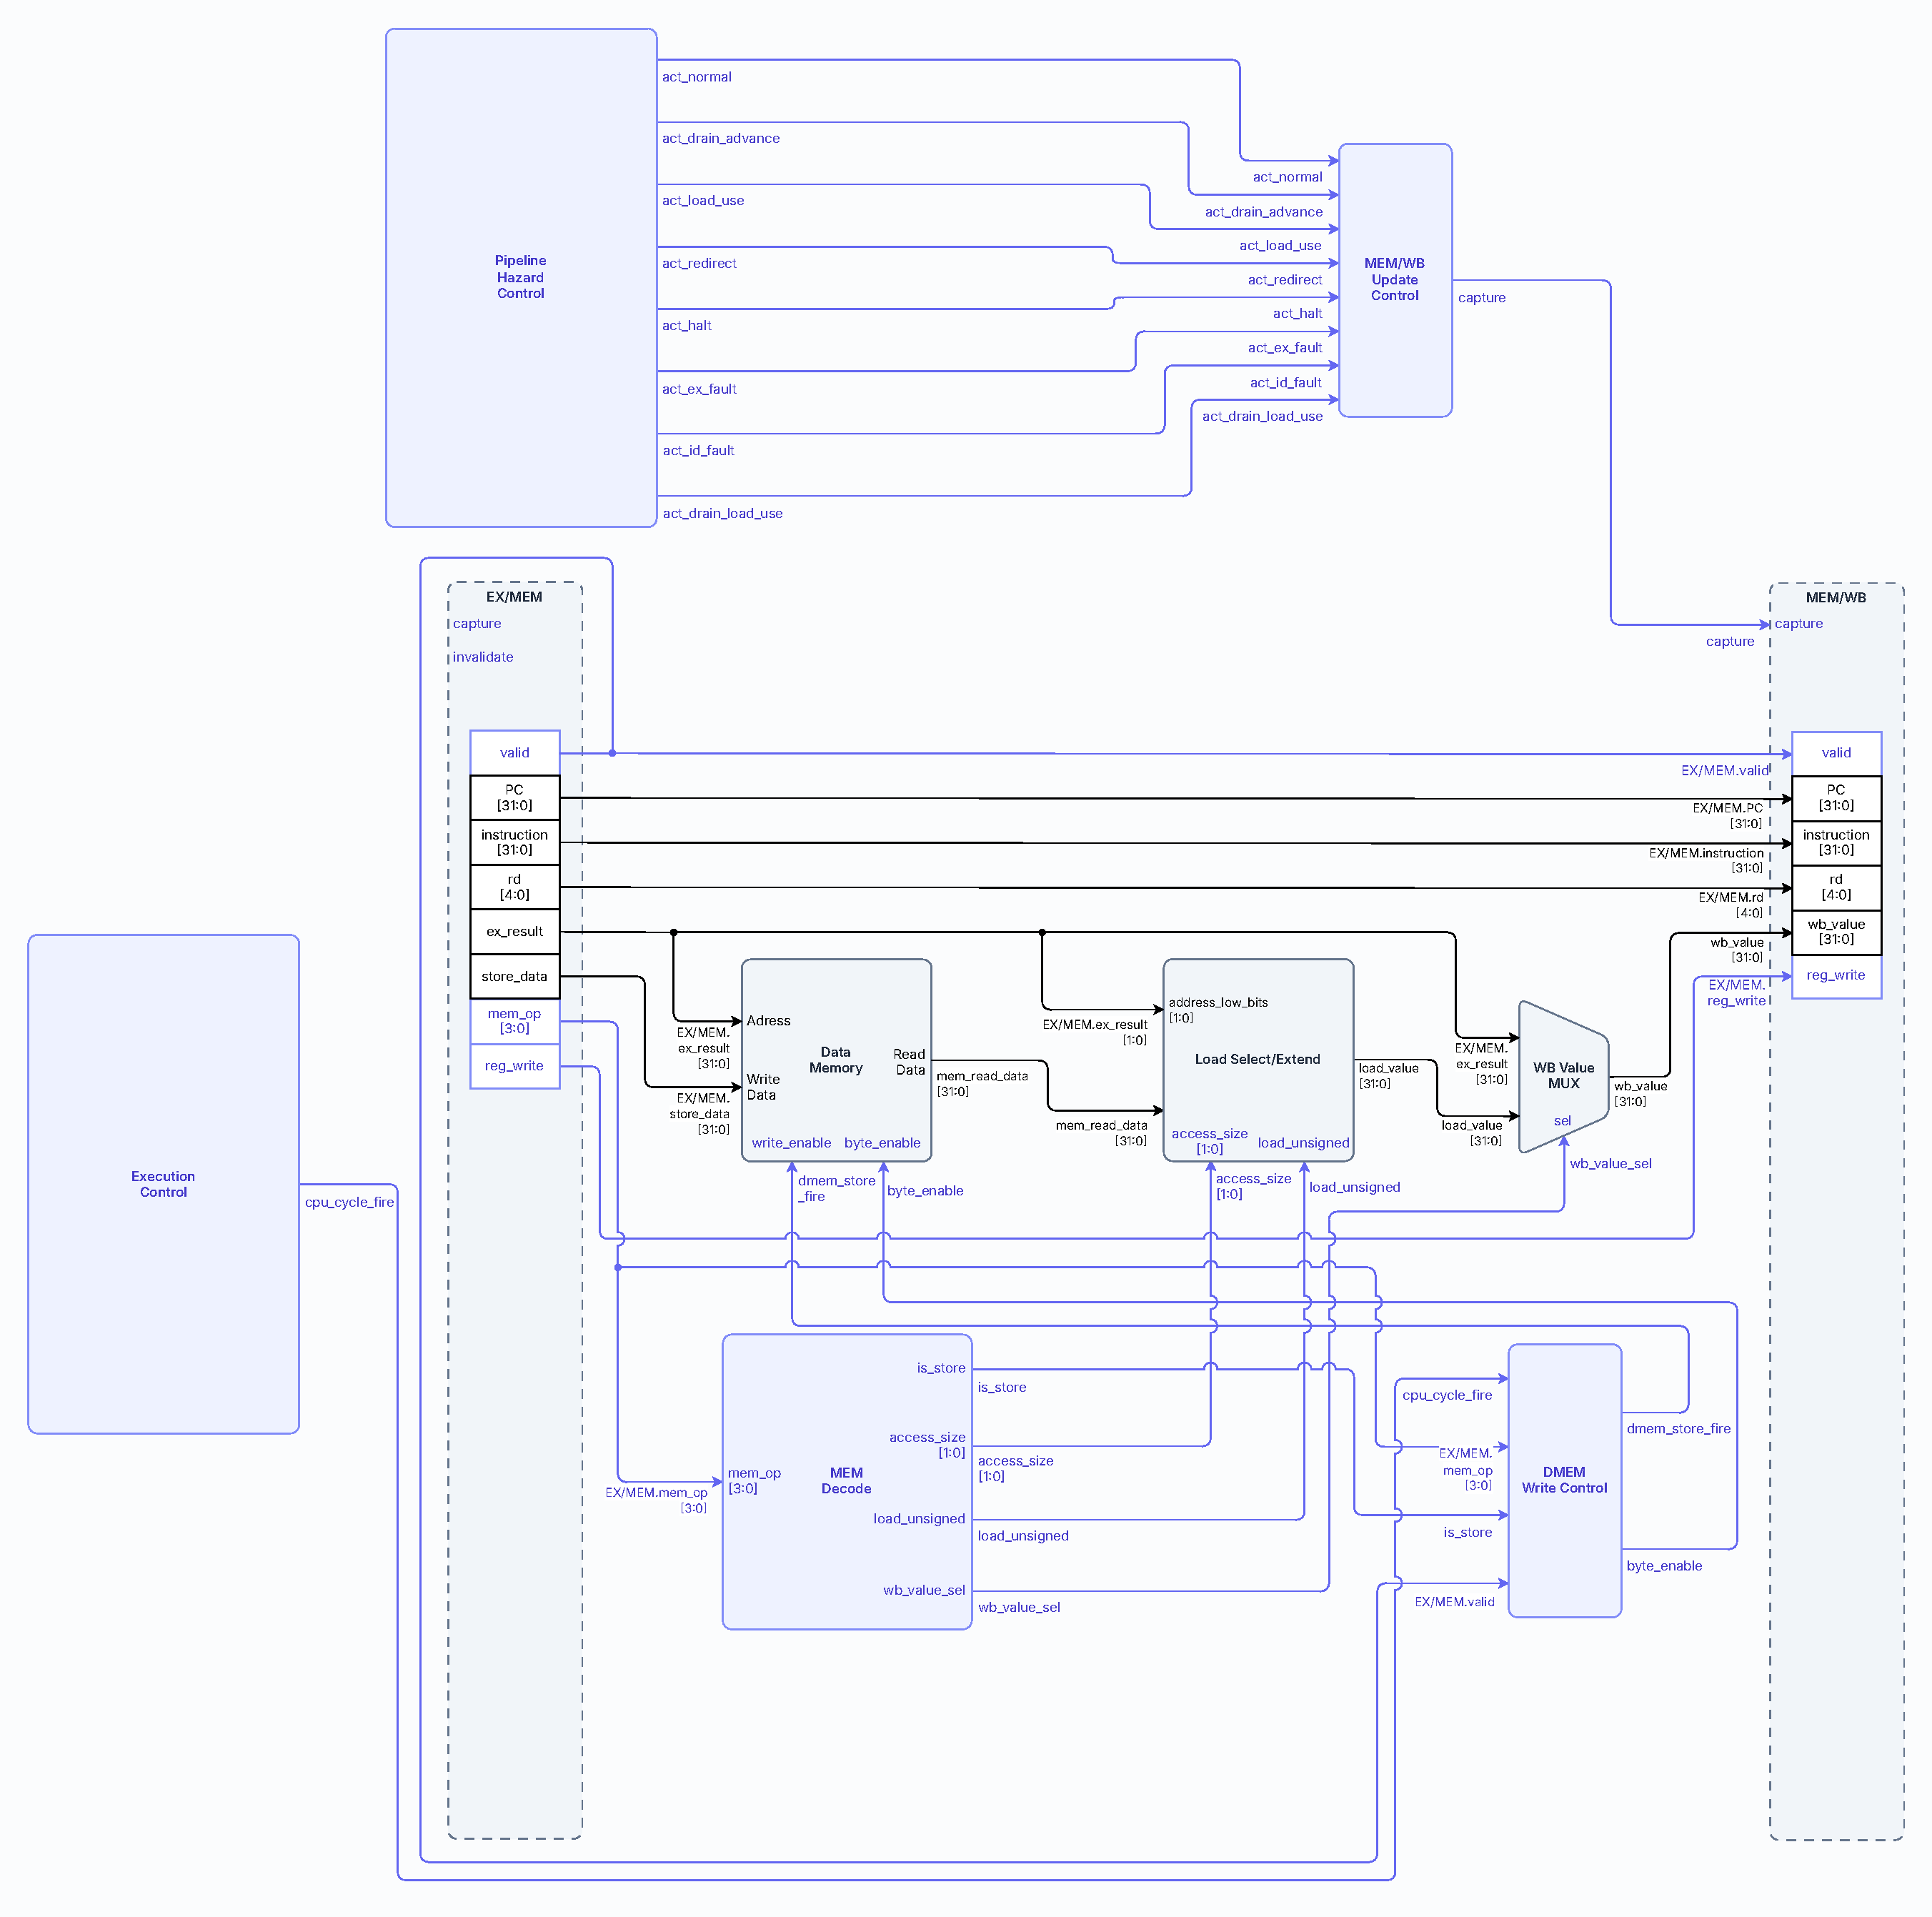
\includegraphics[width=0.80\textwidth]{mem-organizacion.pdf}
  \caption{Organización de MEM: acceso a DMEM, selección y extensión de loads,
  máscara de stores y selección del valor de writeback.}
  \label{fig:etapa-mem}
\end{figure}

\subsection{Loads y selección del dato}

Para un load, \code{EX/MEM.ex_result} es la dirección efectiva. \code{Data
Memory} entrega la palabra alineada de cuatro bytes y \code{Load Select / Extend}
utiliza el offset y el tamaño del acceso para seleccionar el byte, halfword o
word solicitado. Luego aplica extensión con signo o sin signo según
\code{mem_op}. El resultado de 32 bits queda listo para el camino de
writeback.

\subsection{Stores y escritura de DMEM}

Para un store, \code{EX/MEM.ex_result} aporta la dirección y
\code{EX/MEM.store_data} aporta el dato. \code{DMEM Write Control} solo activa
la escritura cuando se cumplen simultáneamente estas condiciones:

\begin{itemize}
  \item el ciclo de CPU es efectivo;
  \item \code{EX/MEM} contiene una entrada válida;
  \item \code{mem_op} identifica un store.
\end{itemize}

La máscara depende del tamaño: un byte para \code{SB}, dos para \code{SH} y
cuatro para \code{SW}. La memoria desplaza esa máscara según los bits bajos de
la dirección y actualiza tanto los datos como sus marcas de validez. Un store
anterior puede completar su efecto en el mismo ciclo en que se confirma el
fault o \code{halt} de una instrucción posterior.

\subsection{Selección del valor de writeback}

La selección de resultados se reparte entre EX y MEM. EX ya eligió entre el
resultado de la ALU, el inmediato y el enlace \code{PC + 4}, y guardó ese valor
en \code{EX/MEM.ex_result}. En MEM, \code{WB Value MUX} selecciona entre ese
resultado y el dato producido por un load. El valor único elegido se captura en
\code{MEM/WB.wb_value}; WB no vuelve a seleccionar su origen.

La estructura detallada de estos caminos se encuentra en
\doc{architecture/cpu/stage_mem.md}{la etapa MEM}.

\section{Write Back (WB)}

WB es la última etapa del recorrido. Recibe desde \code{MEM/WB} el resultado
final de la instrucción y decide si debe hacerlo visible en el banco de
registros. No vuelve a calcular ni a seleccionar el origen del dato: esa
selección ya ocurrió en MEM.

Sus bloques y conexiones principales son:

\begin{itemize}
  \item \textbf{\code{WB Bypass Control}:} forma la condición efectiva de
    escritura y los controles de bypass hacia ID.
  \item \textbf{Puerto de escritura del \code{Register File}:} recibe
    \code{MEM/WB.rd}, \code{MEM/WB.wb_value} y la habilitación de WB.
  \item \textbf{\code{RS1 Bypass MUX} y \code{RS2 Bypass MUX}:} pueden entregar
    a ID el mismo valor de \code{MEM/WB.wb_value} cuando hay una lectura
    coincidente.
  \item \textbf{Registro \code{MEM/WB}:} conserva el resultado final y la
    identidad de la instrucción que WB observa y utiliza.
\end{itemize}

La figura~\ref{fig:etapa-wb} muestra la organización de la etapa.

\begin{figure}[H]
  \centering
  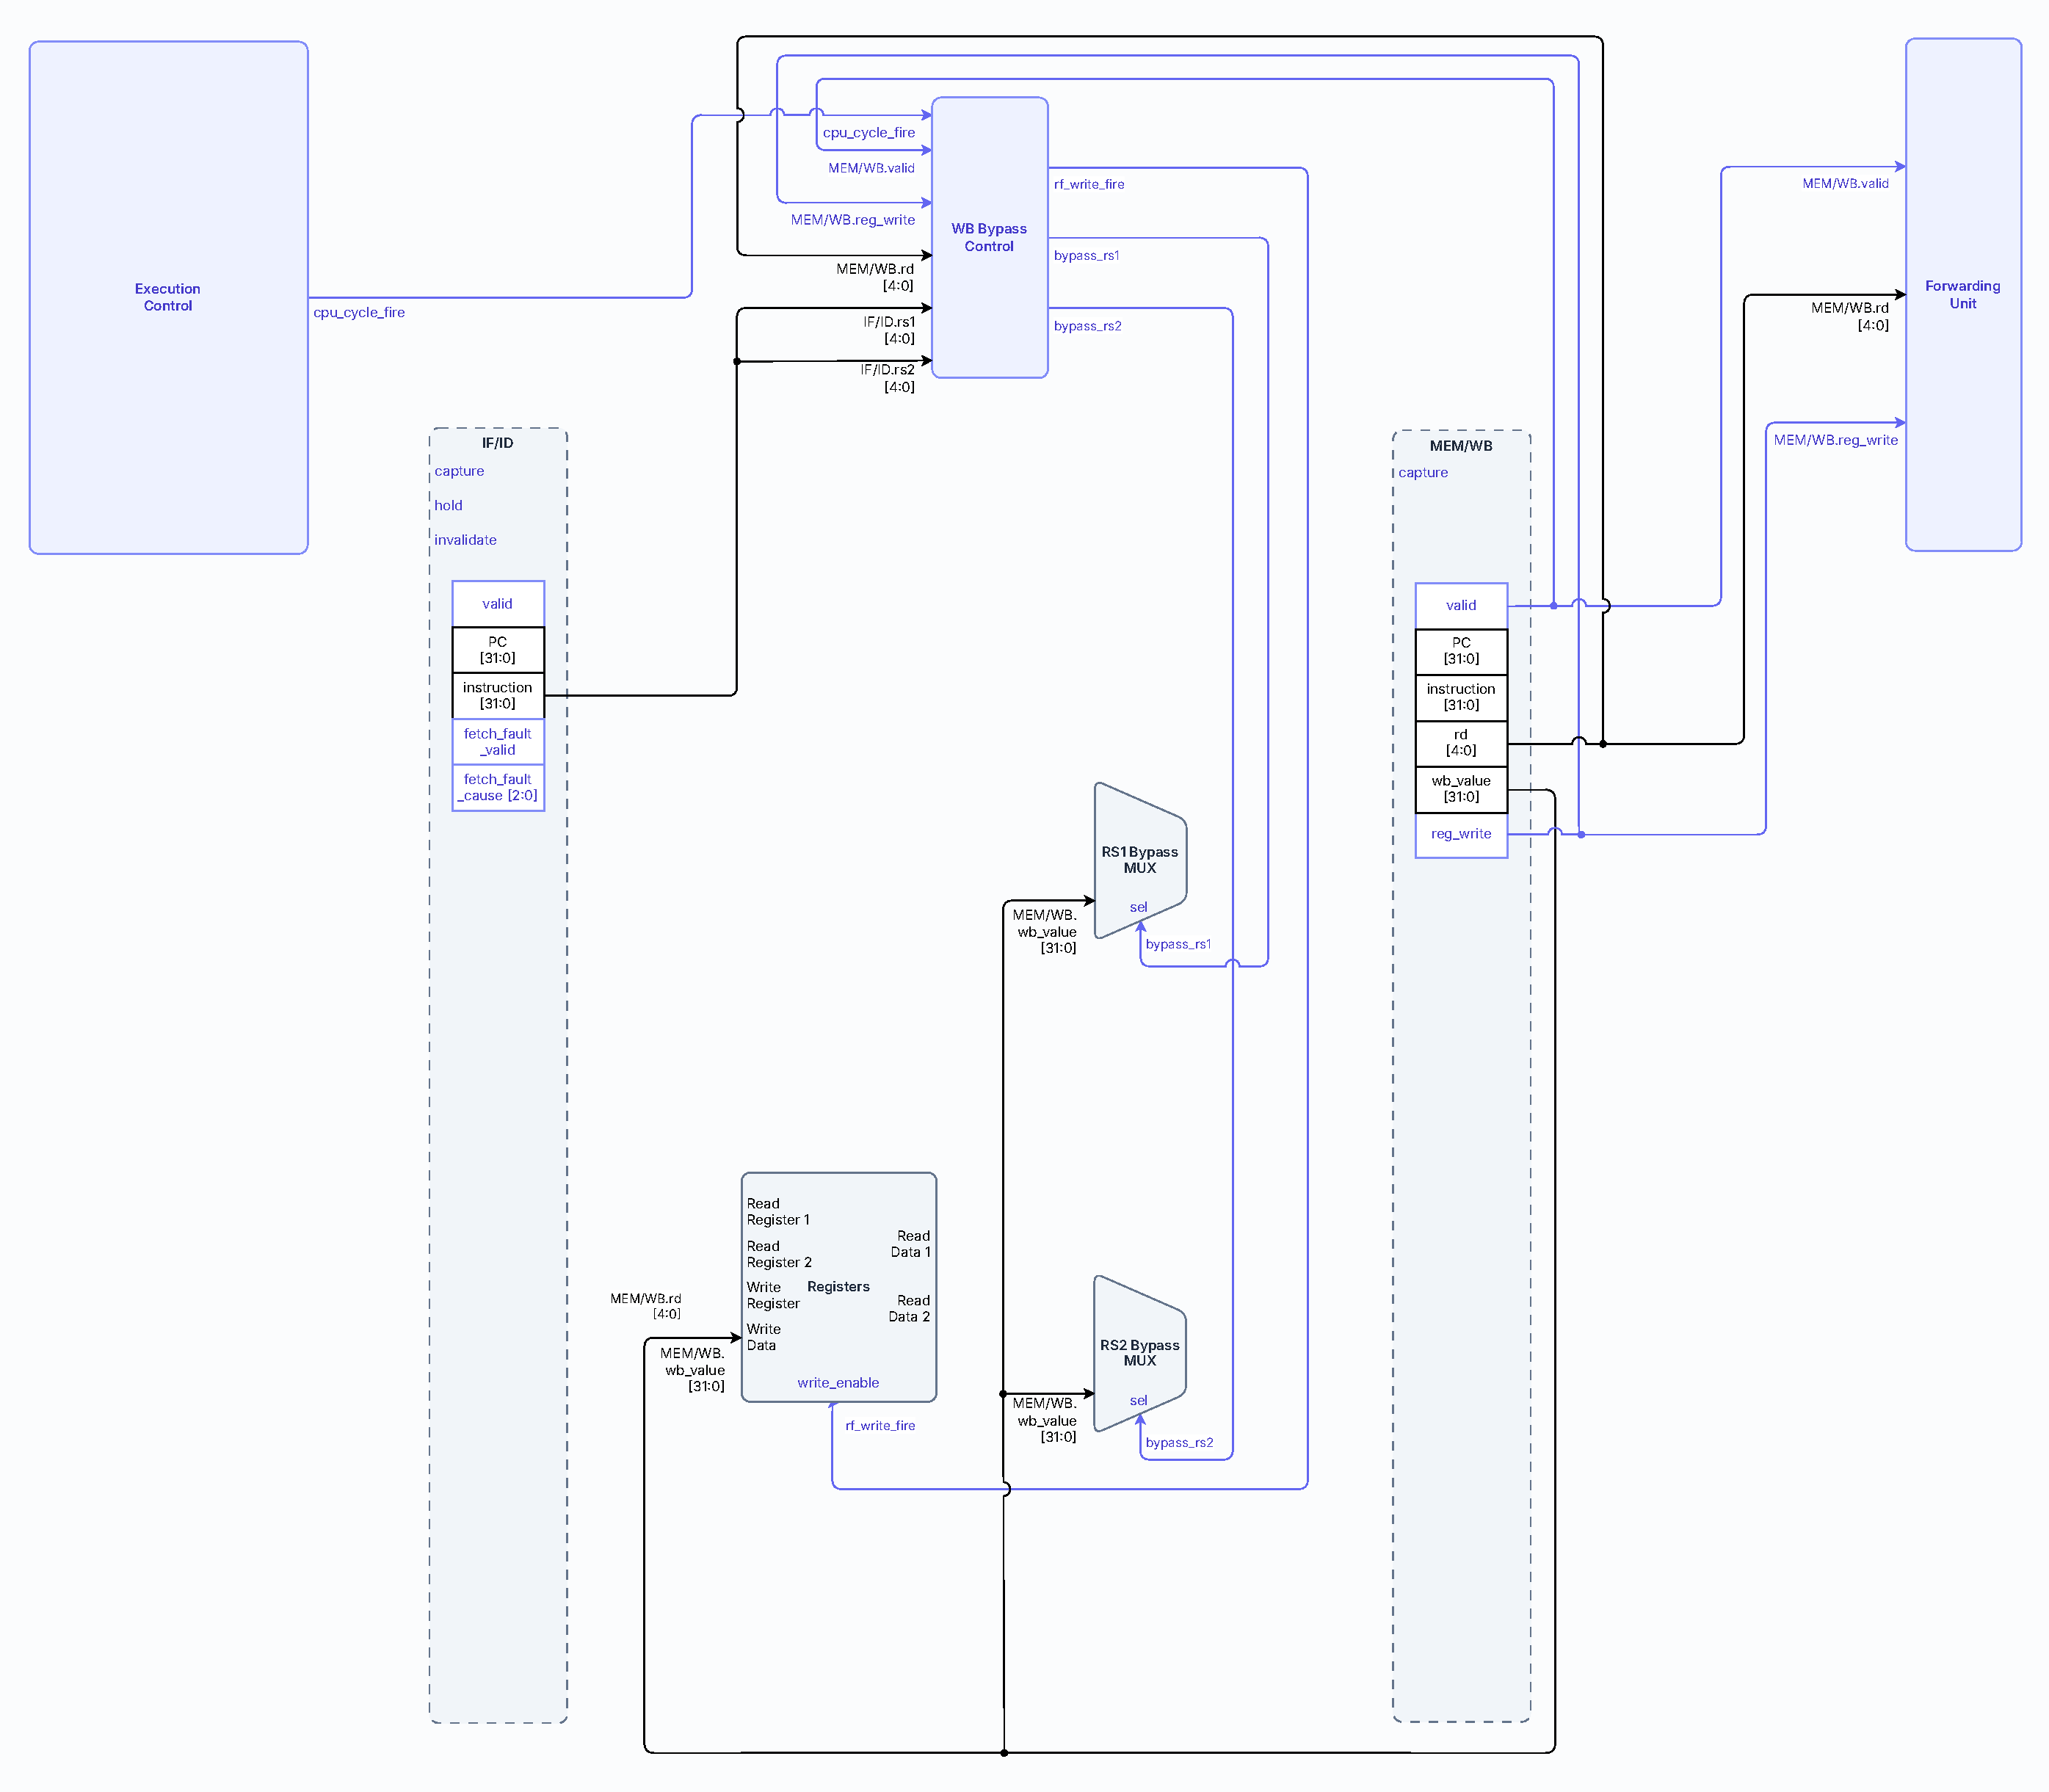
\includegraphics[width=0.92\textwidth]{wb-organizacion.pdf}
  \caption{Organización de WB: escritura del banco de registros y generación
  de los controles de bypass hacia ID.}
  \label{fig:etapa-wb}
\end{figure}

\subsection{Escritura efectiva}

La escritura se realiza de forma síncrona y solo ocurre cuando se cumplen
simultáneamente estas condiciones:

\begin{itemize}
  \item el ciclo de CPU es efectivo;
  \item \code{MEM/WB} contiene una entrada válida;
  \item \code{reg_write} está activo;
  \item el destino es distinto de \code{x0}.
\end{itemize}

Cuando todas se cumplen, WB ejecuta conceptualmente:

\begin{codebox}
RF[MEM/WB.rd] <- MEM/WB.wb_value
\end{codebox}

Una entrada inválida no produce efectos aunque sus campos conserven valores
residuales. Stores y branches pueden atravesar WB con \code{reg_write=0}; en
ese caso solo conservan su identidad para la observación del pipeline.

\subsection{Bypass y forwarding}

La misma escritura efectiva habilita el bypass \tech{WB}$\rightarrow$\tech{ID}.
Si ID lee el registro que WB está escribiendo, el mux correspondiente entrega
directamente \code{MEM/WB.wb_value} en lugar del valor anterior del banco. De
esta forma, el resultado nuevo está disponible en ID durante el mismo ciclo y
la arquitectura no depende de que el almacenamiento sea write-first o
read-first.

Ese mismo \code{MEM/WB.wb_value} también queda disponible para el forwarding
desde MEM/WB hacia EX. WB no crea un valor adicional: reutiliza el resultado
final que MEM ya consolidó, ya provenga de la ALU, de \code{LUI}, del enlace de
un salto o de un load. La condición exacta se detalla en
\doc{architecture/cpu/stage_wb.md}{Etapa WB}.

\section{Registros interetapa y validez}\label{sec:registros-interetapa}

\subsection{Avance y captura}

Los cuatro registros interetapa son \code{if_id_register},
\code{id_ex_register}, \code{ex_mem_register} y \code{mem_wb_register}.
Cada uno captura el trabajo producido por la etapa anterior en el flanco
habilitado. La actualización se basa en los valores previos al flanco; una
instrucción avanza como máximo una etapa por ciclo.

\subsection{Validez y estados del pipeline}

La validez es parte del contrato del pipeline, no un detalle de
implementación. Un registro puede conservar bits residuales en sus otros
campos, pero solo una entrada válida representa una instrucción activa y puede
producir efectos. Esta distinción permite:

\begin{itemize}
  \item representar una burbuja sin ejecutar una instrucción inexistente;
  \item retener una instrucción durante un stall sin invalidarla;
  \item descartar instrucciones de un camino abandonado sin borrar todos sus
    campos;
  \item distinguir un candidato de fault de una instrucción activa.
\end{itemize}

Una entrada inválida no participa en forwarding, bypass ni writeback. En el
caso particular de \code{IF/ID}, \code{valid=0} y
\code{fetch_fault_valid=1} representan un candidato de fault de fetch, no una
instrucción ejecutable. La selección exacta entre captura, retención, burbuja e
invalidación depende de la acción elegida por el control del pipeline.

\subsection{Campos transportados y observables}

Los 34 campos funcionales de los latches suman 504 bits y se observan en Debug.
La tabla~\ref{tab:campos-latches} detalla los campos que transporta cada
registro y el ancho de cada conjunto.

\begin{table}[H]
  \centering
  \footnotesize
  \setlength{\tabcolsep}{3pt}
  \begin{tabularx}{\textwidth}{L{1.7cm}Y r}
    \toprule
    \textbf{Registro} & \textbf{Campos (ancho en bits)} & \textbf{Total} \\
    \midrule
    \code{IF/ID} & \code{valid(1)}, \code{pc(32)}, \code{instruction(32)},
    \code{fetch_fault_valid(1)}, \code{fetch_fault_cause(3)} & 69 \\
    \addlinespace
    \code{ID/EX} & \code{valid(1)}, \code{pc(32)}, \code{instruction(32)},
    \code{rs1(5)}, \code{rs2(5)}, \code{rd(5)}, \code{rs1_value(32)},
    \code{rs2_value(32)}, \code{immediate(32)}, \code{alu_op(6)},
    \code{alu_src(1)}, \code{result_sel(2)}, \code{flow_op(3)},
    \code{mem_op(4)}, \code{reg_write(1)} & 193 \\
    \addlinespace
    \code{EX/MEM} & \code{valid(1)}, \code{pc(32)}, \code{instruction(32)},
    \code{rd(5)}, \code{reg_write(1)}, \code{mem_op(4)}, \code{ex_result(32)},
    \code{store_data(32)} & 139 \\
    \addlinespace
    \code{MEM/WB} & \code{valid(1)}, \code{pc(32)}, \code{instruction(32)},
    \code{rd(5)}, \code{reg_write(1)}, \code{wb_value(32)} & 103 \\
    \bottomrule
  \end{tabularx}
  \caption{Campos funcionales de los registros interetapa.}
  \label{tab:campos-latches}
\end{table}

Estos campos conservan la identidad de la instrucción, los datos que necesita
la etapa siguiente y las señales de control que deben atravesar el pipeline.
La validez determina cuándo ese contenido tiene significado arquitectónico y
también permite que Debug distinga trabajo activo de datos residuales.

\section{Branches, jumps, \code{halt} y faults}

\subsection{Branches, jumps y redirects}

Los branches y jumps se resuelven en EX. \code{Flow Control} compara los
operandos cuando corresponde y produce la solicitud de redirect junto con el
destino calculado. \code{Pipeline Hazard Control} arbitra esa solicitud frente
a los faults, \code{halt} y hazards que puedan aparecer en el mismo ciclo.

Cuando el redirect se confirma, el PC adopta el nuevo destino y se invalidan
las instrucciones más jóvenes que todavía estaban en IF o ID. La instrucción
que originó el cambio de flujo continúa hacia \code{EX/MEM}; así, \code{JAL} y
\code{JALR} pueden conservar su enlace para escribirlo posteriormente.
La figura~\ref{fig:etapa-branch} muestra este recorrido.

\begin{figure}[H]
  \centering
  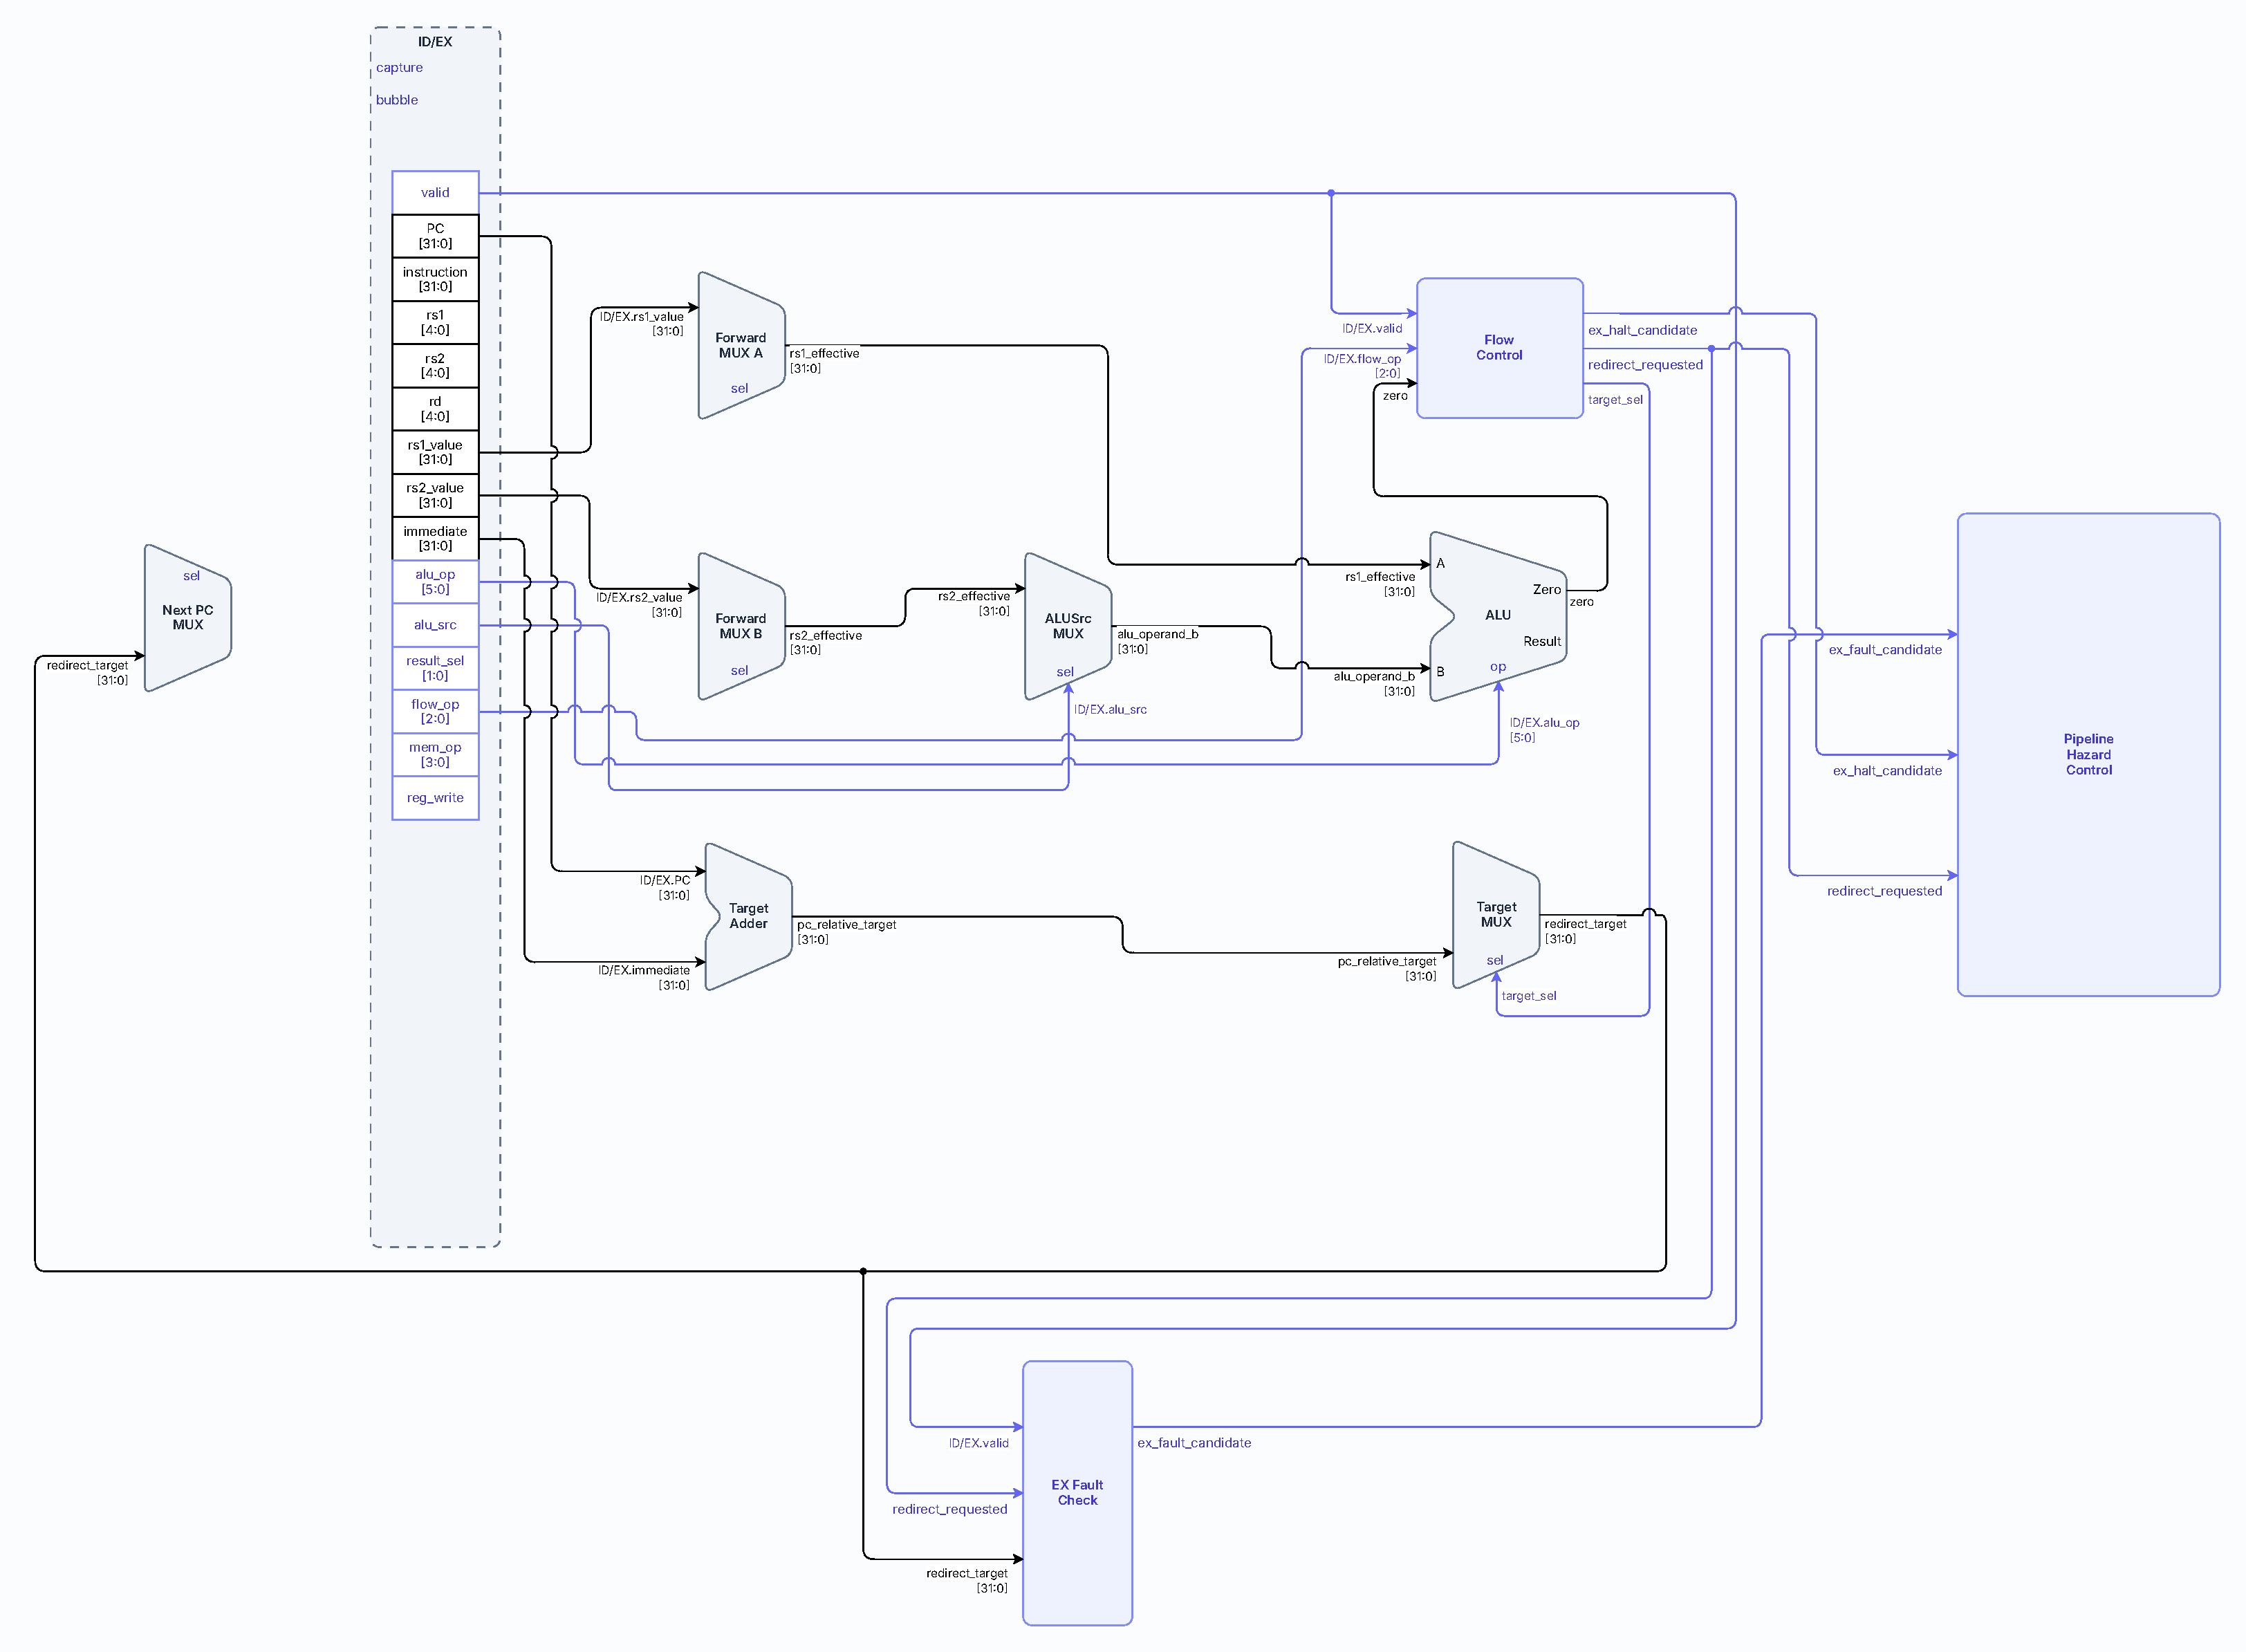
\includegraphics[width=0.92\textwidth]{ex-branch.pdf}
  \caption{Recorrido de un branch en EX: comparación, cálculo del destino y
  selección del próximo PC.}
  \label{fig:etapa-branch}
\end{figure}

\subsection{Origen y transporte de faults}

Un fault puede detectarse en tres puntos del pipeline:

\begin{itemize}
  \item \textbf{IF:} una búsqueda desalineada o fuera de la capacidad o de la
    imagen confirmada produce un candidato de fault de fetch.
  \item \textbf{ID:} una instrucción ilegal o un candidato de fetch transportado
    por \code{IF/ID} produce un candidato de fault de ID.
  \item \textbf{EX:} se detecta una dirección desalineada o fuera de rango en
    un acceso a DMEM, o un destino de control inválido.
\end{itemize}

La detección solo produce un candidato. La confirmación ocurre en un ciclo
efectivo, después de que \code{Pipeline Hazard Control} comprueba que ninguna
instrucción anterior produjo un evento con mayor prioridad. La figura
~\ref{fig:fetch-fault} muestra cómo un candidato de IF se transporta por
\code{IF/ID} antes de confirmarse en ID.

\subsection{Prioridad y precisión}

La confirmación respeta el orden del programa. La prioridad entre eventos es:

\begin{enumerate}
  \item fault propio de EX;
  \item \code{halt} en EX;
  \item redirect en EX;
  \item fault en ID;
  \item dependencia \code{load-use};
  \item avance normal.
\end{enumerate}

Cuando se confirma un fault, la instrucción causante y las posteriores se
descartan, mientras que las anteriores conservan sus efectos válidos. La causa
y el PC de la instrucción que falló se capturan una sola vez por sesión y se
conservan hasta el estado terminal. El diseño no necesita rollback: la
precisión se obtiene controlando qué instrucciones pueden producir efectos.

Las causas se codifican con tres bits. El código \code{011} queda reservado y
no representa una causa válida:

\begin{center}
  \begin{tabular}{clp{8.5cm}}
    \toprule
    \textbf{Código} & \textbf{Causa} & \textbf{Descripción} \\
    \midrule
    \code{000} & Instrucción desalineada & El PC no es múltiplo de cuatro. \\
    \code{001} & Falla de acceso a instrucción & La búsqueda de cuatro bytes queda fuera de la capacidad de IMEM o de la imagen confirmada. \\
    \code{010} & Instrucción ilegal & La palabra obtenida no coincide con ninguna codificación implementada. \\
    \code{011} & Reservado & No corresponde a una causa válida. \\
    \code{100} & Load desalineado & La dirección no cumple la alineación requerida por el tamaño del load. \\
    \code{101} & Falla de acceso a load & Alguno de los bytes solicitados por el load queda fuera del rango de DMEM. Una dirección dentro de DMEM que nunca fue escrita no produce este fault: el load obtiene cero lógico. \\
    \code{110} & Store desalineado & La dirección no cumple la alineación requerida por el tamaño del store. \\
    \code{111} & Falla de acceso a store & Alguno de los bytes que escribiría el store queda fuera del rango de DMEM. \\
    \bottomrule
  \end{tabular}
\end{center}

\subsection{\code{halt} y drenado}

\code{halt} se confirma en EX y no ingresa válidamente a \code{EX/MEM}. Las
instrucciones más jóvenes se invalidan, mientras que las anteriores que ya
están en MEM o WB continúan y pueden completar sus efectos. El sistema entra
en drenado y alcanza el estado terminal cuando el pipeline queda vacío.

\begin{figure}[H]
  \centering
  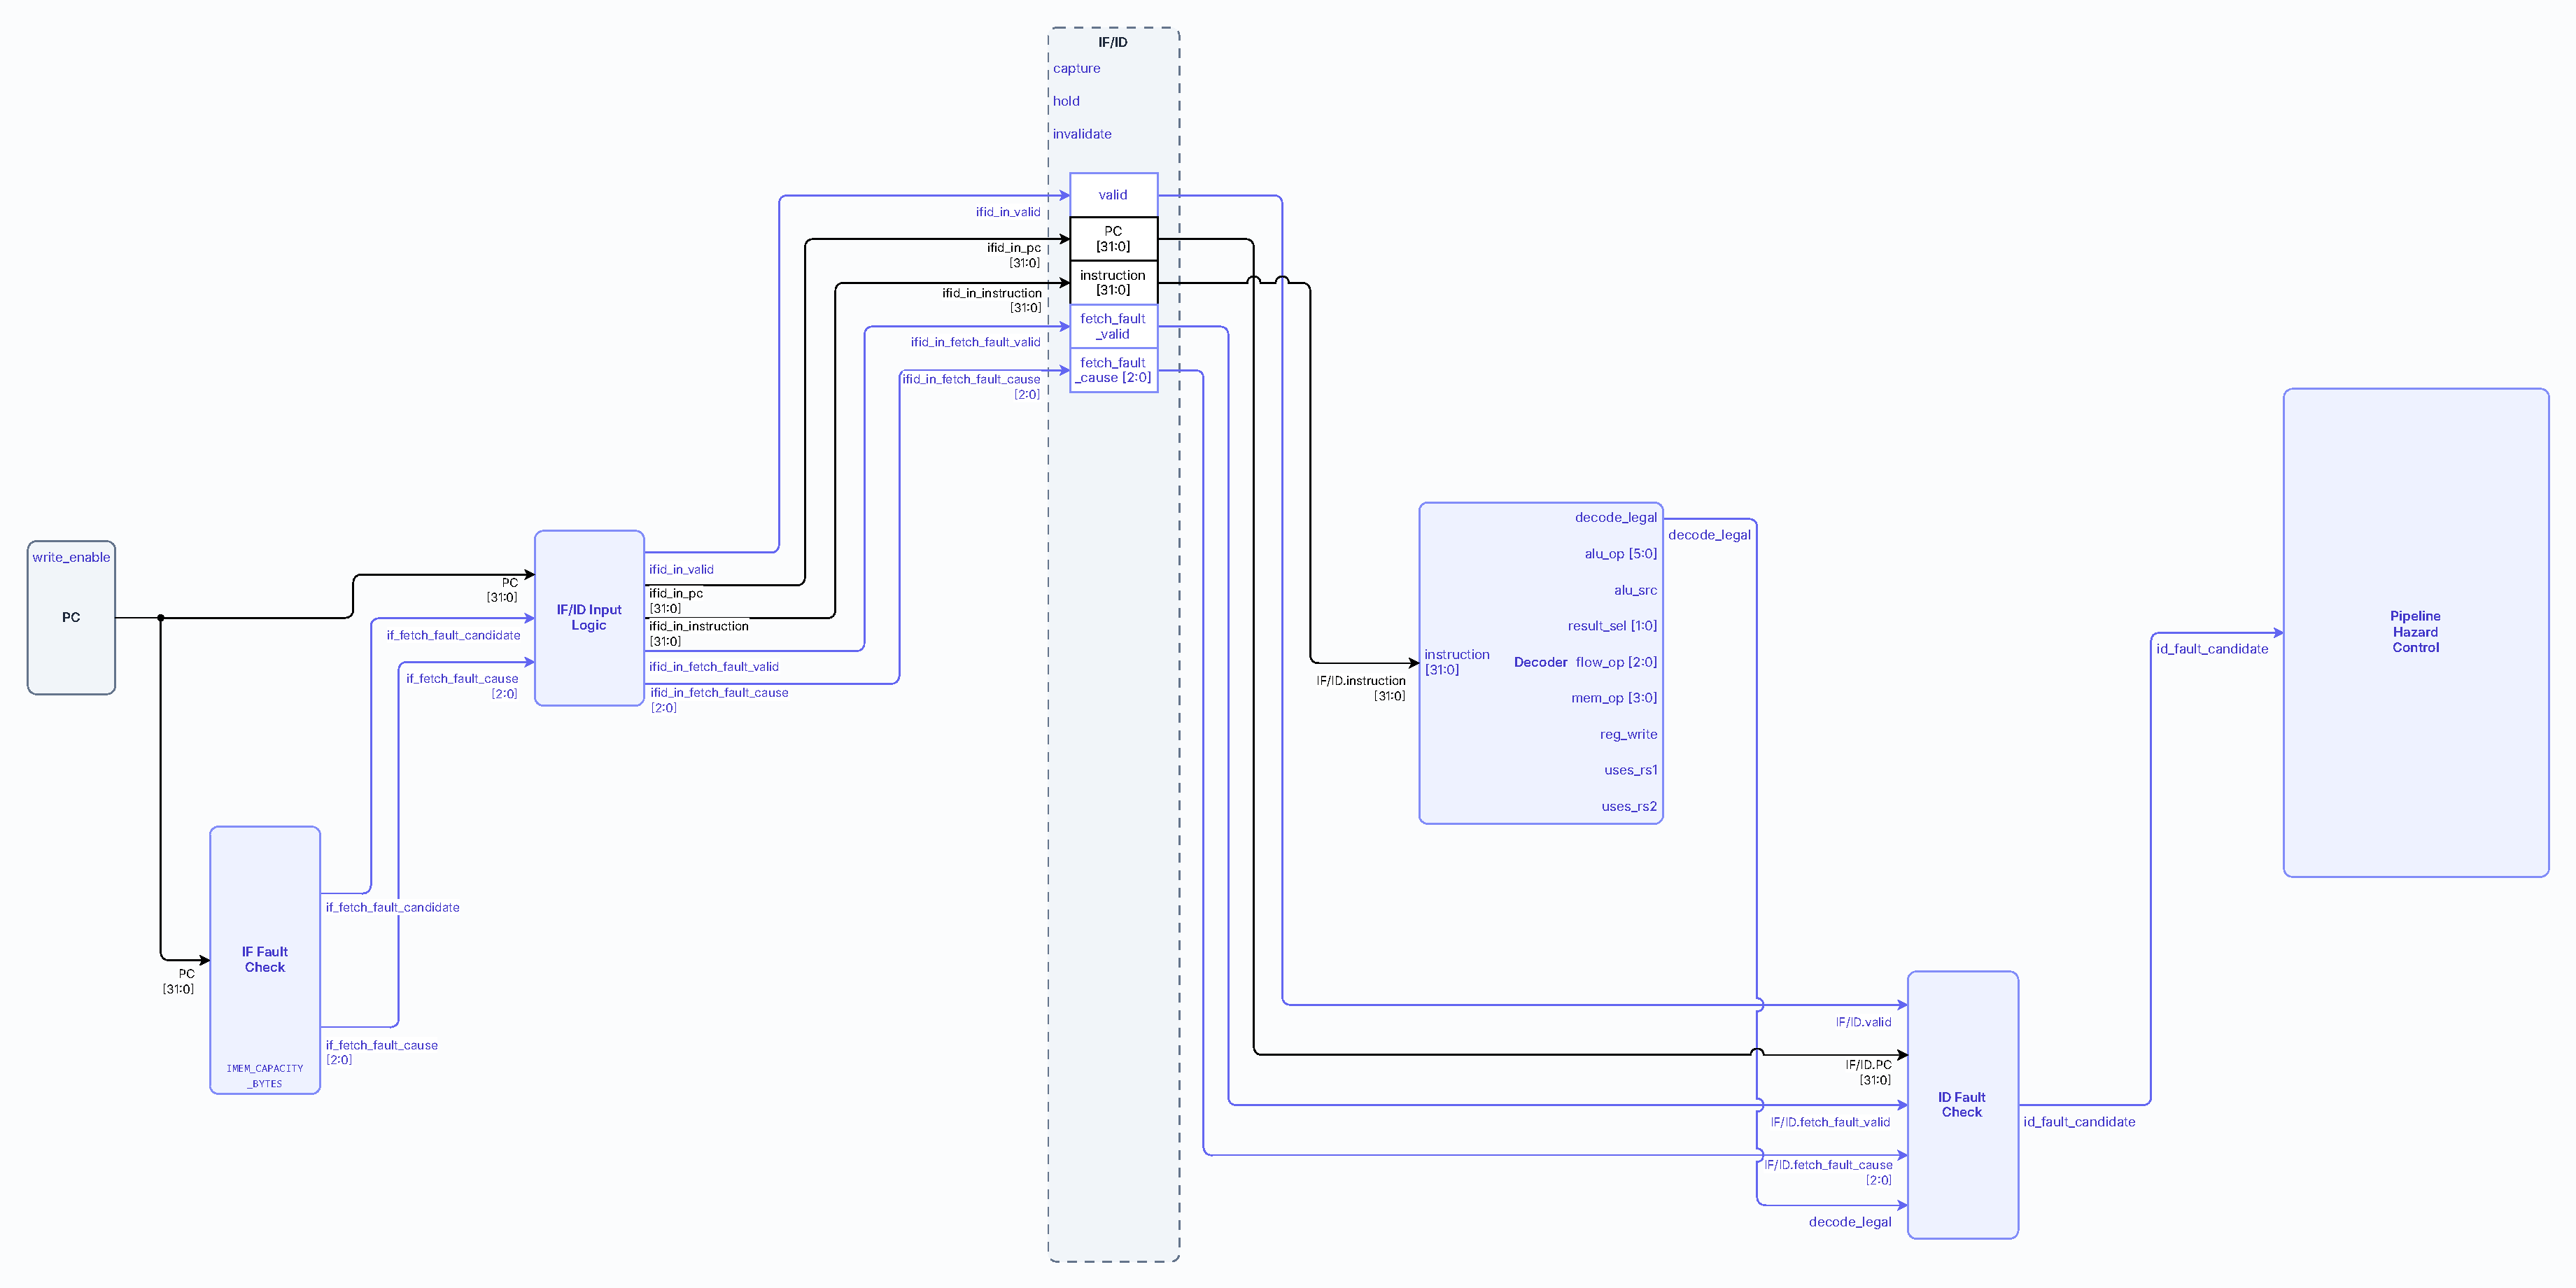
\includegraphics[width=0.95\textwidth]{fetch-fault.pdf}
  \caption{Recorrido del candidato de fault de fetch y su transporte por
  IF/ID.}
  \label{fig:fetch-fault}
\end{figure}


\chapter{Memorias, carga y preparación}\label{chap:memorias}
\section{Dos memorias independientes}

La CPU utiliza dos memorias lógicamente independientes, cada una con su propio
contenido y recorrido de acceso:

\begin{itemize}
  \item \textbf{\tech{IMEM}:} conserva la imagen confirmada de instrucciones
    que IF puede buscar durante la ejecución.
  \item \textbf{\tech{DMEM}:} conserva los datos de la sesión sobre los que
    operan las instrucciones de load y store.
\end{itemize}

Ambas comienzan en la dirección \code{0x00000000}, pero no comparten el mismo
espacio de direcciones. Por eso, una dirección numérica igual puede identificar
una posición de IMEM y otra distinta de DMEM.

La separación permite que IF lea una instrucción mientras MEM accede a los datos
en el mismo ciclo. No se produce un hazard estructural entre el fetch y el
acceso a datos, y cada memoria recibe como máximo una solicitud de la CPU por
ciclo. El contrato completo se encuentra en
\doc{architecture/memory/memory_architecture.md}{Arquitectura de memoria}.

\begin{figure}[H]
  \centering
  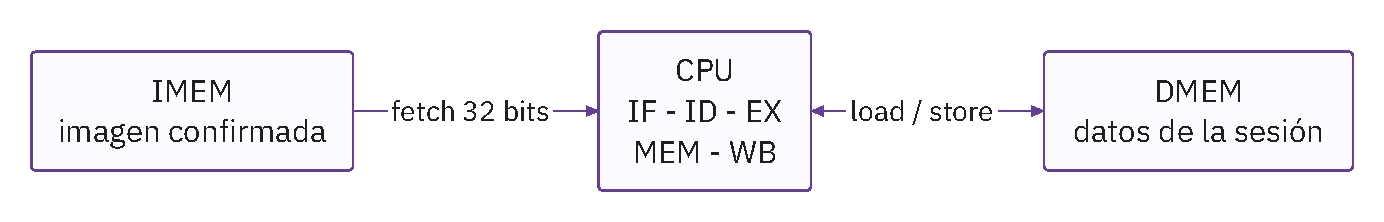
\includegraphics[width=0.95\textwidth]{memorias.pdf}
  \caption{Espacios independientes de instrucciones y datos.}
  \label{fig:memorias}
\end{figure}

\section{Instruction Memory}

IMEM almacena la imagen de instrucciones que utiliza el procesador. Es una
memoria direccionada por bytes: el PC representa la dirección del primer byte
del fetch y cada instrucción ocupa cuatro direcciones consecutivas, \code{PC},
\code{PC + 1}, \code{PC + 2} y \code{PC + 3}. Por ejemplo, si
\code{PC = 0x08}, la instrucción se forma con los bytes de \code{0x08} a
\code{0x0B}.

Durante la ejecución, la lectura de IMEM es combinacional mientras que durante la carga, la
escritura es síncrona. Ninguna de las dos operaciones agrega una latencia
variable ni un stall específico de memoria.

\subsection{Imagen ejecutable}

En este capítulo, llamaremos a una \emph{imagen} como el conjunto de bytes de programa que la
PC envía mediante \code{LOAD} y que el sistema recibe y escribe en IMEM. La imagen incluye solo el tramo cargado del programa:
su tamaño se conserva en \code{loaded_image_size_bytes} y ese límite determina
qué bytes pueden buscarse como instrucciones.

La imagen ejecutable es una única región inicial y continua. Para que pueda
publicarse, debe cumplir todas estas condiciones:

\begin{itemize}
  \item comienza en \code{0x00000000};
  \item no está vacía;
  \item no tiene huecos;
  \item su tamaño es múltiplo de cuatro;
  \item no supera \code{IMEM_CAPACITY_BYTES}.
\end{itemize}

Una sesión preparada comienza a ejecutar desde \code{PC = 0}, el inicio de la
imagen. El tamaño confirmado se conserva en \code{loaded_image_size_bytes}; de
ese valor se derivan \code{image_valid} y la cantidad de instrucciones
disponibles.

La región ejecutable comienza en la dirección cero y termina en el último byte
del tamaño confirmado. Solo los fetches completamente contenidos en ese
intervalo pueden ingresar al pipeline. El contenido físico que quede fuera del
límite no pertenece a la imagen vigente.

\subsection{Validación de fetch}

Para que un fetch sea válido deben cumplirse tres condiciones:

\begin{itemize}
  \item el PC debe estar alineado a cuatro bytes;
  \item los cuatro bytes deben caber dentro de la capacidad física de IMEM;
  \item los cuatro bytes deben pertenecer al tramo confirmado de la imagen.
\end{itemize}

La condición de rango se expresa como:

\begin{codebox}
if_fetch_range_valid =
    image_valid
    && ({1'b0, PC} + 33'd4 <= IMEM_CAPACITY_BYTES)
    && ({1'b0, PC} + 33'd4 <= loaded_image_size_bytes)
\end{codebox}

La comparación utiliza aritmética de 33 bits para conservar el extremo completo
del acceso y evitar que una dirección fuera de rango haga alias con una dirección
baja. Si la validación falla, IF genera un candidato de fault de fetch; ID lo
confirma después de respetar el orden de las instrucciones anteriores.

\subsection{Carga y publicación}

\subsubsection{Recepción y escritura}

El \code{Loader} recibe la imagen byte a byte y reconstruye cada palabra de
cuatro bytes. Durante el proceso de carga conserva los tres primeros bytes que le llegan en un registro de 24 bits y, al
recibir el cuarto, forma la palabra y la escribe en IMEM. La escritura solo se
habilita cuando el \code{Loader} posee la memoria y el índice de palabra es
válido.

\subsubsection{Fin de la carga}

La señal \code{load_ok} certifica que la última palabra se escribió en el
flanco de la última entrega válida. Este evento indica que terminó la
transferencia y la escritura de IMEM; la imagen todavía no es ejecutable.

\subsubsection{Publicación de la imagen}

La imagen se publica cuando termina la preparación de la sesión. En el flanco
que consume \code{prepare_done}, el sistema captura el tamaño validado en
\code{loaded_image_size_bytes}. A partir de ese momento, ese tamaño delimita
los fetches que pueden considerarse parte de la imagen ejecutable.

Si la carga o la preparación no terminan correctamente, no se publica una
imagen nueva. Una solicitud \code{LOAD} rechazada conserva la imagen y la
sesión anteriores.

\section{Data Memory}

DMEM almacena los datos que utiliza el programa durante la sesión. La etapa MEM
accede a ella mediante loads y stores de uno, dos o cuatro bytes, según la
instrucción. Está direccionada por bytes, de manera que cada dirección
identifica una posición de un byte.

La lectura es combinacional, por lo que el dato queda disponible sin esperar
un flanco de reloj adicional. En cambio, un store autorizado actualiza los
bytes correspondientes en un flanco de reloj.

Cada byte tiene una marca de validez que indica si fue escrito durante la
sesión actual. Al preparar una nueva sesión se limpian estas marcas y, a medida
que los stores escriben datos, se activan las correspondientes a los bytes
modificados. Así, la lectura devuelve el dato almacenado cuando su marca está
activa y cero cuando está inactiva, aunque físicamente quede un valor de una
sesión anterior.

\subsection{Lanes y little-endian}

Los bytes de DMEM se organizan en filas de cuatro posiciones. Cada posición de
una fila se denomina \emph{lane} y almacena un byte con su correspondiente
marca de validez. Para ubicar una dirección de byte, los dos bits menos
significativos seleccionan el lane y los bits restantes identifican la fila:

\begin{codebox}
lane = direccion[1:0]
fila = direccion >> 2
\end{codebox}

Por ejemplo, las direcciones \code{0x04}, \code{0x05}, \code{0x06} y
\code{0x07} pertenecen a la fila 1 y corresponden, respectivamente, a los
lanes 0, 1, 2 y 3. Esta organización permite leer los cuatro bytes de una fila
como una palabra de 32 bits y seleccionar los bytes que necesita un load. Para
un store, permite identificar los lanes que deben actualizarse.

Los valores de varios bytes se almacenan en orden \emph{little-endian}: el
byte menos significativo ocupa la dirección más baja. Por ejemplo, al
almacenar la palabra \code{0x12345678} desde la dirección $A$, sus bytes
quedan distribuidos de la siguiente manera:

\begin{table}[H]
  \centering
  \small
  \begin{tabular}{cc}
    \toprule
    \textbf{Dirección} & \textbf{Byte} \\
    \midrule
    \code{A + 0} & \code{0x78} \\
    \code{A + 1} & \code{0x56} \\
    \code{A + 2} & \code{0x34} \\
    \code{A + 3} & \code{0x12} \\
    \bottomrule
  \end{tabular}
  \caption{Orden little-endian de un valor de 32 bits.}
  \label{tab:little-endian}
\end{table}

La figura~\ref{fig:memoria-organizacion} muestra, a la derecha, las filas y
lanes de DMEM. La fila resaltada representa el ejemplo anterior con
\code{A = 0x04}, y los círculos indican la validez de cada byte. A la izquierda
se muestra la organización de IMEM para comparar ambas memorias.

\begin{figure}[H]
  \centering
  \begin{tikzpicture}[
      cell/.style={draw=codeviolet, fill=codeback, rounded corners=1pt,
        minimum width=1.22cm, minimum height=0.70cm, inner sep=1pt,
        font=\ttfamily\footnotesize, anchor=center},
      title/.style={font=\small\bfseries, anchor=center},
      note/.style={font=\footnotesize, anchor=center},
      rowlabel/.style={font=\ttfamily\footnotesize, anchor=east},
      valid/.style={circle, draw=codeviolet, fill=codeviolet,
        minimum size=2.4pt, inner sep=0pt},
      invalid/.style={circle, draw=codeviolet, fill=white,
        minimum size=2.4pt, inner sep=0pt},
      arrow/.style={-{Latex[length=2mm]}, thick, draw=codeviolet}
    ]
    % (a) IMEM: palabras de 32 bits, direccionadas por PC >> 2.
    \node[title] at (2.05,1.45) {(a) IMEM};
    \node[note] at (2.05,1.05) {256 palabras de 32 bits};
    \foreach \i/\label in {0/+0, 1/+1, 2/+2, 3/+3} {
      \node[note] at ({0.5+\i*1.3},0.52) {\label};
      \node[cell] (im\i) at ({0.5+\i*1.3},0) {b\i};
    }
    \node[note, anchor=east] at (-0.15,0) {PC};
    \node[note] at (2.05,-0.90) {palabra de 32 bits};
    \node[note] at (2.05,-1.30) {índice de palabra = \code{PC >> 2}};

    % (b) DMEM: cuatro lanes de bytes y una marca de validez por byte.
    \node[title] at (9.95,1.45) {(b) DMEM};
    \node[note] at (9.95,1.05) {4 lanes de bytes $\times$ 512 filas};
    \foreach \lane/\label in {0/0, 1/1, 2/2, 3/3} {
      \node[note] at ({8.15+\lane*1.30},0.52) {lane \label};
    }
    \foreach \row/\addr/\ba/\bb/\bc/\bd/\validflag in {
        0/0x0000/00/00/00/00/0,
        1/0x0004/78/56/34/12/1,
        2/0x0008/00/00/00/00/0,
        3/0x000C/00/00/00/00/0
      } {
        \node[rowlabel] at (7.55,{-\row*1.05}) {\addr};
        \foreach \lane/\cellvalue in {0/\ba, 1/\bb, 2/\bc, 3/\bd} {
          \node[cell] at ({8.15+\lane*1.30},{-\row*1.05}) {\cellvalue};
          \node[invalid] at ({7.75+\lane*1.30},{-\row*1.05+0.23}) {};
        }
      }
    \foreach \lane in {0, 1, 2, 3} {
      \node[valid] at ({7.75+\lane*1.30},{-0.82}) {};
    }
    \draw[codeviolet, thick, rounded corners=2pt] (7.45,-1.50) rectangle (12.75,-0.60);
    \node[note, anchor=west] at (13.15,-1.05) {$A=0x0004$};
  \end{tikzpicture}
  \caption{Organización de las memorias. Cada celda representa un byte; en
  DMEM, el círculo superior izquierdo indica la validez de ese byte: lleno si
  fue escrito y vacío si todavía se lee como cero. La fila resaltada muestra la
  palabra \code{0x12345678} almacenada en \code{0x0004}.}
  \label{fig:memoria-organizacion}
\end{figure}


Los lanes describen la organización lógica de DMEM; la implementación
utiliza arrays inferidos para representar los datos y sus marcas.

\subsection{Loads y stores}

Los loads y stores acceden a DMEM a partir de una dirección efectiva calculada
en EX. En esa etapa también se comprueba la alineación y el rango del acceso,
de modo que MEM recibe las operaciones válidas junto con la información
necesaria para leer o escribir los bytes solicitados.

\subsubsection{Lectura mediante loads}

Para un load, DMEM entrega los cuatro bytes lógicos de la fila que contiene la
dirección efectiva. Por ejemplo, si la dirección es \code{0x05}, la memoria
entrega la fila que abarca las direcciones \code{0x04} a \code{0x07}. Luego,
\code{Load Select/Extend} utiliza los dos bits inferiores de la dirección para
identificar la posición inicial y selecciona uno, dos o cuatro bytes según la
instrucción.

El resultado debe ocupar 32 bits para continuar hacia writeback. En los loads
de uno o dos bytes, el bloque completa los bits superiores con ceros o con
copias del bit de signo, según corresponda. La tabla~\ref{tab:loads} resume
los tamaños y las extensiones de cada instrucción:

\begin{table}[H]
  \centering
  \small
  \begin{tabular}{lll}
    \toprule
    \textbf{Instrucción} & \textbf{Bytes} & \textbf{Resultado} \\
    \midrule
    \code{LB}  & 1 & extensión con signo \\
    \code{LBU} & 1 & extensión con cero \\
    \code{LH}  & 2 & ensamblado y extensión con signo \\
    \code{LHU} & 2 & ensamblado y extensión con cero \\
    \code{LW}  & 4 & palabra completa \\
    \bottomrule
  \end{tabular}
  \caption{Selección y extensión de loads.}
  \label{tab:loads}
\end{table}

La figura~\ref{fig:mem-load} muestra este recorrido, desde la lectura de DMEM
hasta la selección y extensión del valor que continúa hacia writeback.

\begin{figure}[H]
  \centering
  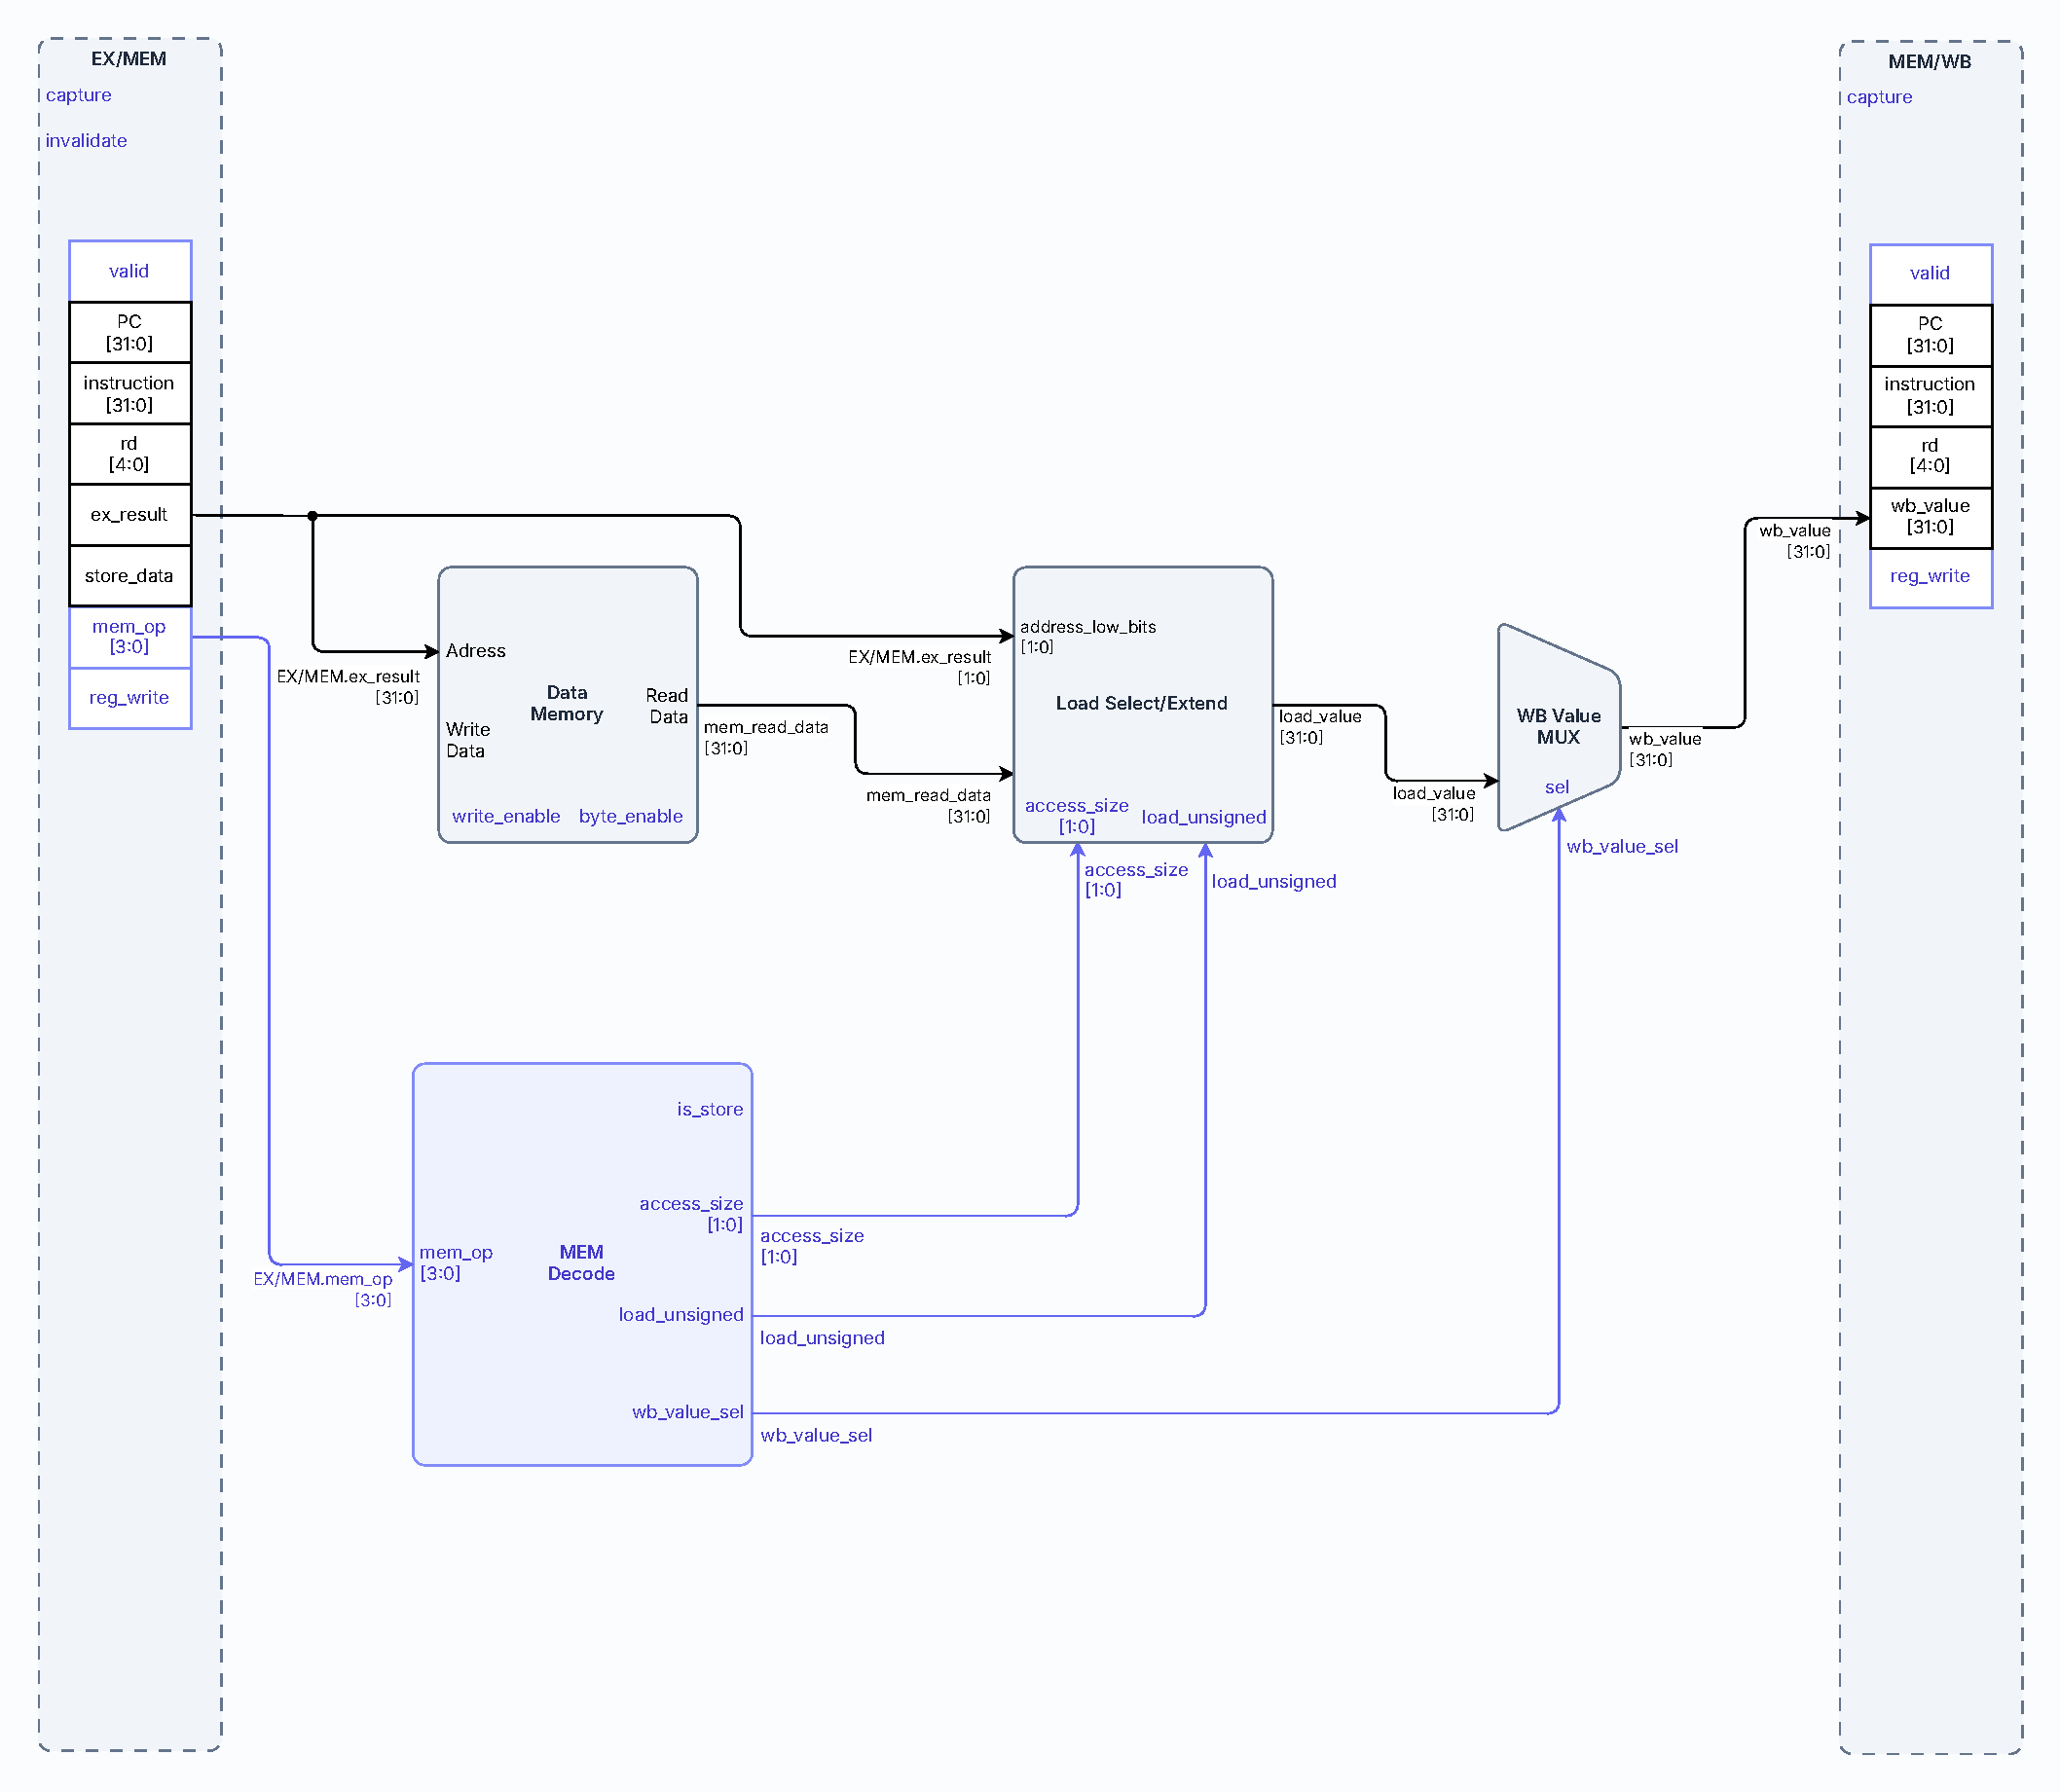
\includegraphics[width=0.72\textwidth]{mem-load.pdf}
  \caption{Recorrido de un load en MEM: lectura de DMEM, selección de bytes y
  extensión del resultado.}
  \label{fig:mem-load}
\end{figure}

\subsubsection{Escritura mediante stores}

Un store llega a MEM con la dirección efectiva y el dato que debe almacenar.
Según la instrucción, el control genera una máscara de cuatro bits que indica
cuántos bytes bajos del dato se escribirán: uno para \code{SB}, dos para
\code{SH} y cuatro para \code{SW}.

DMEM utiliza los dos bits inferiores de la dirección para ubicar esos bytes y
la máscara en los lanes correspondientes. Por ejemplo, un \code{SB} en la
dirección \code{0x05} escribe el byte menos significativo del dato en el
lane 1 de la fila 1. En el flanco autorizado se actualizan juntos los datos y
las marcas de los lanes seleccionados, mientras que los demás conservan su
contenido y validez.

Todos los bytes de un store válido se escriben en el mismo flanco. Además, la
marca se activa incluso cuando el valor escrito es cero, ya que registra si el
byte fue utilizado durante la sesión. La figura~\ref{fig:mem-store} muestra el
recorrido de la dirección, el dato y la máscara hasta su escritura en DMEM.

\begin{figure}[H]
  \centering
  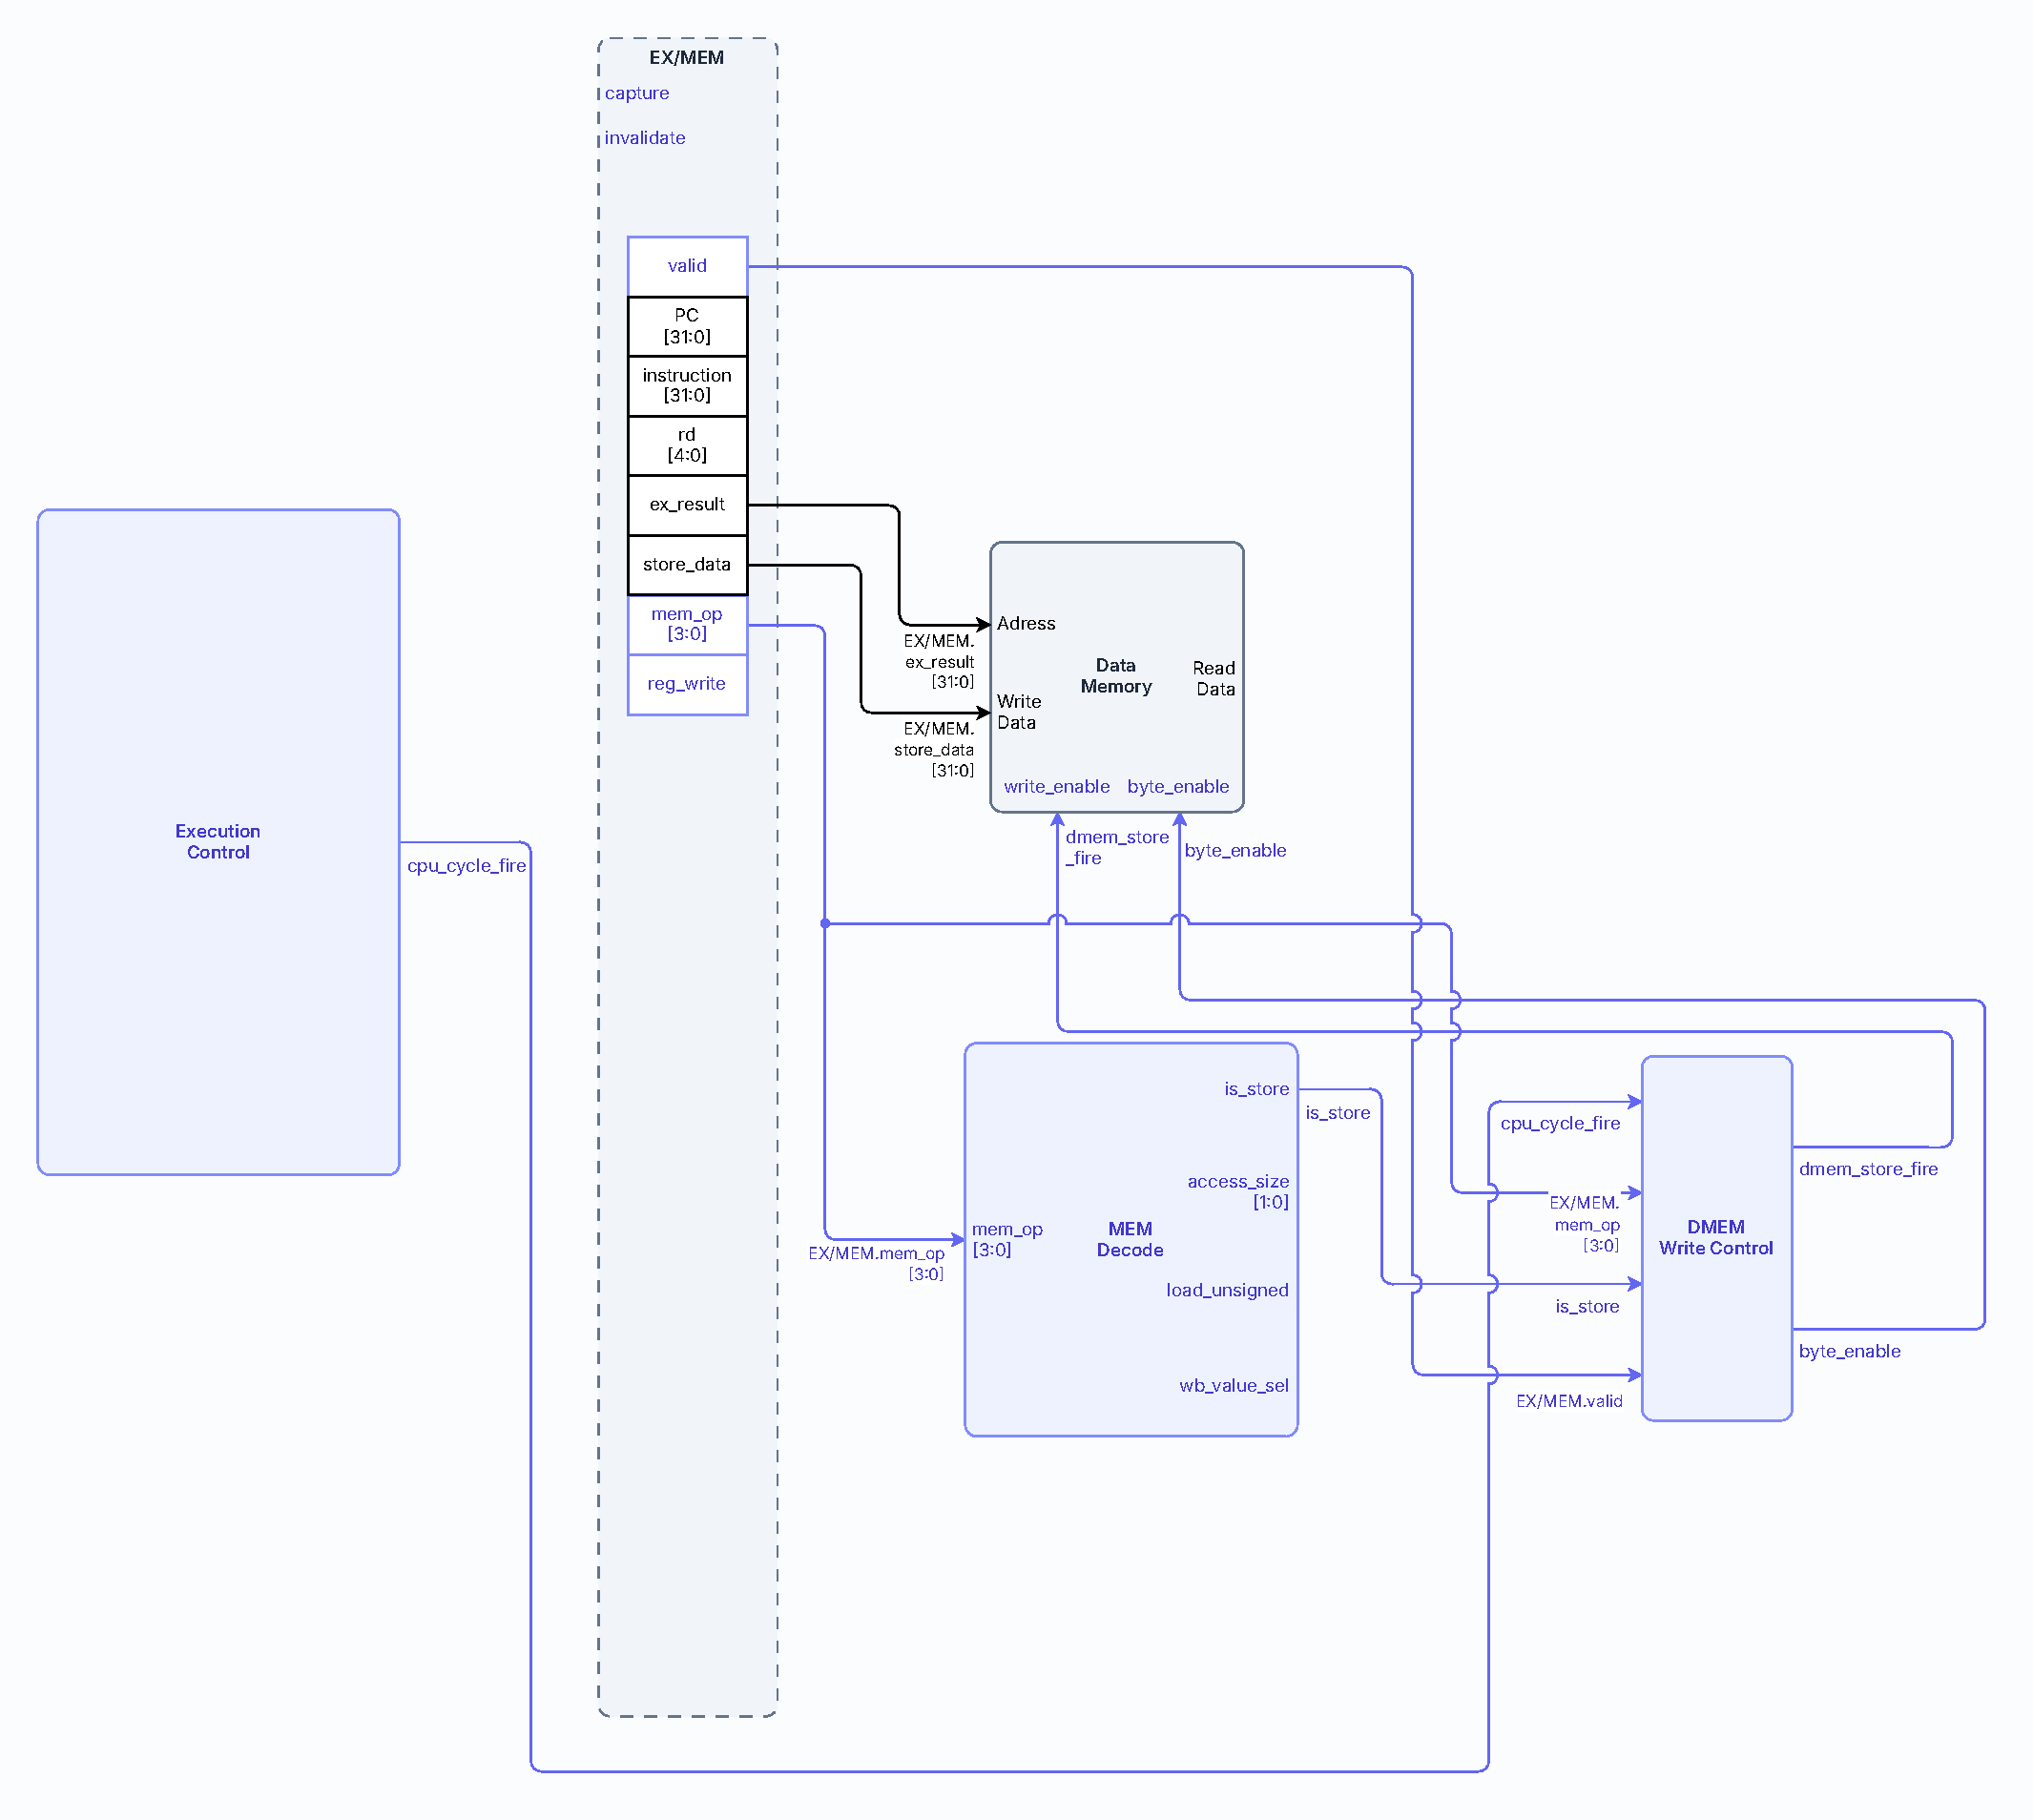
\includegraphics[width=0.72\textwidth]{mem-store.pdf}
  \caption{Recorrido de un store en MEM: dirección, dato, máscara de bytes y
  actualización conjunta de dato y validez.}
  \label{fig:mem-store}
\end{figure}

\section{Direcciones, alineación y rango}

Para que un acceso sea válido, su dirección debe cumplir la alineación exigida
por el tamaño de la operación y todos los bytes solicitados deben pertenecer a
la región permitida. En los loads y stores, estas comprobaciones se realizan
en EX sobre la dirección efectiva. Para el fetch se valida el PC y la región
de la imagen ejecutable, como se explicó en la sección de IMEM.

\subsection{Dirección efectiva}

La dirección efectiva de un load o store se obtiene sumando el valor efectivo
de \code{rs1} y el inmediato de la instrucción. La suma utiliza aritmética de
32 bits, por lo que conserva sus 32 bits inferiores:

\begin{codebox}
effective_address = (rs1_effective + immediate) mod 2^32
\end{codebox}

Por ejemplo, si \code{rs1} vale \code{0xffffffff} y el inmediato es 1, la
dirección resultante es \code{0x00000000}. El acarreo de esta suma no produce
un fault por sí mismo; la dirección resultante se utiliza para comprobar la
alineación y el rango.

\subsection{Alineación}

Los accesos de varios bytes deben comenzar en una dirección múltiplo de su
tamaño. Por eso, un acceso de dos bytes comienza en una dirección par y uno de
cuatro bytes, en una dirección múltiplo de cuatro. El fetch también requiere
un PC alineado a cuatro bytes. La tabla~\ref{tab:alineacion} resume estas
condiciones:

\begin{table}[H]
  \centering
  \small
  \begin{tabular}{ll}
    \toprule
    \textbf{Acceso} & \textbf{Condición} \\
    \midrule
    \code{LB}, \code{LBU}, \code{SB} & sin restricción adicional \\
    \code{LH}, \code{LHU}, \code{SH} & \code{address[0] = 0} \\
    \code{LW}, \code{SW} & \code{address[1:0] = 00} \\
    fetch & \code{PC[1:0] = 00} \\
    \bottomrule
  \end{tabular}
  \caption{Condiciones de alineación.}
  \label{tab:alineacion}
\end{table}

\subsection{Rango del acceso}

Además de estar alineado, un load o store debe tener todos sus bytes dentro de
DMEM. Si la dirección efectiva es el primer byte y \code{N} es el tamaño del
acceso en bytes, se comprueba que el extremo posterior a la región no supere
la capacidad de la memoria:

\begin{codebox}
dmem_range_valid =
    ({1'b0, effective_address} + N) <= DMEM_CAPACITY_BYTES
\end{codebox}

Esta suma y la comparación se realizan con 33 bits para conservar el posible
acarreo al calcular el extremo. Así, una región que supera el límite de las
direcciones de 32 bits no se confunde con una región ubicada al comienzo de la
memoria. Por ejemplo, en una DMEM de 2048 bytes, una palabra que comienza en
la dirección 2044 ocupa los últimos cuatro bytes y está dentro del rango,
mientras que una palabra que comienza en 2048 queda fuera de él.

\subsection{Accesos inválidos}

Una dirección desalineada genera un fault de alineación y una región fuera de
rango genera un fault de acceso. Si una misma operación incumple ambas
condiciones, se informa la desalineación. Cuando hay faults de instrucciones
distintas, prevalece el de la instrucción anterior en el programa. En particular,
un store inválido no modifica datos ni marcas, por lo que no deja una escritura
parcial.

\section{Temporización y acceso a las memorias}

\subsection{Temporización de lectura y escritura}

Las lecturas de IMEM y DMEM son combinacionales: a partir de la dirección
presentada, el dato queda disponible durante el mismo ciclo. Las escrituras,
en cambio, son síncronas y actualizan la memoria en el flanco de reloj cuando
están habilitadas. Como ambas memorias son independientes, IF puede leer una
instrucción mientras MEM accede a datos en ese mismo ciclo.

Este esquema permite que la CPU utilice las memorias sin esperar una respuesta
de latencia variable ni insertar un stall específico por memoria. Cuando el
pipeline está en \code{HOLD}, no se autorizan ciclos de CPU y un store retenido
en MEM no repite su escritura. El reset también inhibe las escrituras.

\subsection{Coordinación de los accesos}

Además de la CPU, otros bloques utilizan las memorias para cargar el programa,
preparar la sesión y observar sus datos. El control del sistema coordina esos
accesos según la actividad en curso, como muestra la
tabla~\ref{tab:ownership}.

\begin{table}[H]
  \centering
  \small
  \begin{tabularx}{\textwidth}{L{1.6cm}L{3.1cm}Y}
    \toprule
    \textbf{Memoria} & \textbf{Bloque} & \textbf{Acceso} \\
    \midrule
    IMEM & Loader & Escribe la imagen durante la carga. \\ \addlinespace
    IMEM & CPU & Lee instrucciones durante la ejecución. \\ \addlinespace
    DMEM & Preparación & Limpia las marcas de validez al iniciar una sesión. \\ \addlinespace
    DMEM & CPU & Lee o escribe datos durante la ejecución. \\ \addlinespace
    DMEM & Debug & Lee datos y marcas cuando la CPU no ejecuta ciclos. \\
    \bottomrule
  \end{tabularx}
  \caption{Bloques que acceden a las memorias y función de cada acceso.}
  \label{tab:ownership}
\end{table}

Estos accesos se coordinan por etapas de funcionamiento. Durante la carga, el
\code{Loader} escribe IMEM y la CPU no ejecuta instrucciones. Luego, la
preparación limpia las marcas de DMEM antes de iniciar la sesión. Durante la
ejecución, la CPU utiliza ambas memorias; cuando Debug necesita observar DMEM,
la CPU queda detenida y un selector presenta la dirección de Debug al camino de
lectura compartido. Así, cada bloque accede a la memoria cuando le corresponde
y se evitan accesos incompatibles sobre una misma memoria.

\section{Perfiles y parametrización}

Las capacidades de IMEM y DMEM se configuran por separado antes de elaborar el
diseño. Cada una se expresa en bytes y determina el rango de direcciones de su
memoria. El dominio arquitectónico admite capacidades entre 4 y $2^{32}$ bytes,
siempre que sean múltiplos de cuatro, ya que las memorias se organizan en
palabras o filas de cuatro bytes.

Los anchos de los índices se calculan a partir de la capacidad configurada y
conservan al menos un bit, incluso para la configuración mínima. La
tabla~\ref{tab:perfiles} presenta los dos perfiles utilizados en el proyecto:

\begin{table}[H]
  \centering
  \small
  \begin{tabular}{lrrl}
    \toprule
    \textbf{Perfil} & \textbf{IMEM} & \textbf{DMEM} & \textbf{Alcance} \\
    \midrule
    \code{REFERENCE} & \SI{1024}{\byte} & \SI{2048}{\byte} &
    Simulación, síntesis, implementación y placa. \\
    \code{ALT_1000} & \SI{1000}{\byte} & \SI{1000}{\byte} &
    Elaboración y simulaciones de parametrización. \\
    \bottomrule
  \end{tabular}
  \caption{Perfiles de memoria.}
  \label{tab:perfiles}
\end{table}

\code{REFERENCE} es el perfil utilizado para la implementación en FPGA, mientras
que \code{ALT_1000} se usa en simulación para comprobar la parametrización con
capacidades que no son potencias de dos. La PC y la FPGA deben utilizar el
mismo perfil para interpretar los límites de las memorias de forma coherente.

Una configuración fuera del dominio arquitectónico se rechaza antes de
elaborar los arrays. Si una capacidad es válida para la arquitectura, pero una
realización concreta no puede admitirla, se informa como error de
configuración y no como un fault del programa.

\section{Reprogramación y estado inicial}

Una vez configurada la FPGA, el sistema puede ejecutar distintos programas sin
modificar el diseño del procesador. Para cambiar de programa, la PC envía una
nueva imagen de instrucciones mediante el comando \code{LOAD} y el sistema la
almacena en IMEM. Así, la reprogramación cambia el contenido que ejecuta la
CPU sin resintetizar el diseño ni volver a cargar el bitstream.

La imagen y la sesión representan dos aspectos distintos de la ejecución: la
imagen contiene las instrucciones cargadas, mientras que la sesión comprende
una ejecución de esas instrucciones y el estado que se va generando en el
procesador y en DMEM. Una misma imagen puede ejecutarse en más de una sesión,
siempre que se prepare nuevamente el estado inicial antes de comenzar.

Cuando se acepta una nueva carga, el sistema abandona la sesión vigente e
invalida la imagen anterior. El \code{Loader} escribe entonces la nueva imagen
en IMEM y, una vez recibida, comienza la preparación de la sesión. Esta etapa
establece el estado inicial desde el que se ejecutará el programa:

\begin{itemize}
  \item \code{PC = 0};
  \item banco de registros en cero lógico;
  \item registros interetapa inválidos;
  \item DMEM con todas sus marcas de validez en cero;
  \item \code{cycle_count = 0};
  \item metadatos de fault sin vigencia.
\end{itemize}

Al limpiar las marcas de DMEM, la preparación garantiza que la nueva sesión
observe cero en las posiciones que todavía no escribió, aunque el almacenamiento
conserve datos de la sesión anterior. Del mismo modo, solo los bytes confirmados
de la nueva imagen se consideran instrucciones ejecutables.

Una vez completadas la carga y la preparación, la imagen se publica y queda
disponible para ejecutar. La secuencia completa se describe en
\doc{architecture/session/execution_control.md}{Control de ejecución y sesión}.


\chapter{Control de ejecución y sesión}\label{chap:control-ejecucion}
El control de ejecución coordina la carga de programas, el inicio de las
sesiones y el avance del procesador. También determina qué ocurre cuando se
confirma una terminación, se solicita un reinicio o se vuelve a ejecutar una
imagen ya cargada. Para hacerlo, combina las órdenes recibidas desde la PC con
el estado de la sesión y las señales producidas por el pipeline.

\section{Reloj físico y ciclo efectivo}

Todo el sistema utiliza un reloj físico común, que sigue funcionando mientras
se carga un programa, se espera una orden o se transmite una respuesta de
Debug. La CPU, sin embargo, no necesariamente avanza en cada flanco: solo
realiza un \emph{ciclo efectivo} cuando el control activa
\code{cpu_cycle_fire}.

Un ciclo efectivo no equivale necesariamente a completar una instrucción. En
él, el pipeline puede avanzar normalmente, resolver una dependencia o un cambio
de flujo, confirmar \code{halt} o un fault, o completar trabajo durante el
drenado. Todos estos casos cuentan como ciclos de CPU.

Cuando \code{cpu_cycle_fire} está inactiva, la CPU permanece retenida, salvo
que una operación global, como reset, una carga aceptada o la preparación de
una sesión, modifique su estado. De esta manera, la actividad de UART y Debug
puede continuar sin agregar ciclos a la ejecución observada.

\section{FSM global de sesión}

La FSM global registra en qué fase se encuentra el sistema: por ejemplo, si
espera una imagen, prepara una sesión, ejecuta instrucciones o termina el
trabajo que queda en el pipeline. A partir de esa fase y de los eventos que
recibe, decide qué órdenes puede aceptar y cuándo autorizar un ciclo de CPU.

La FSM genera señales de control que utilizan el PC, el banco de registros,
las memorias y los demás bloques para actualizar su estado en el flanco
correspondiente. La implementación se distribuye entre \code{global_fsm.sv} y
\code{execution_control.sv}.

La tabla~\ref{tab:estados} presenta sus catorce estados. Para facilitar la
lectura de las transiciones, los diagramas que siguen muestran por separado la
carga, la ejecución y el drenado. Cada vista omite las permanencias sin eventos;
además, \code{RESET} tiene prioridad desde cualquier estado y una \code{LOAD}
aceptada prevalece sobre las transiciones locales.

\begin{table}[H]
  \centering
  \small
  \begin{tabularx}{\textwidth}{L{4.2cm}Y}
    \toprule
    \textbf{Estado} & \textbf{Significado} \\
    \midrule
    \code{NO_IMAGE} & No existe una imagen ejecutable confirmada. \\
    \code{LOADING} & Se recibe y valida una imagen nueva. \\
    \code{PREPARING_READY} & Se prepara la primera sesión de una imagen
    recién cargada. \\
    \code{READY} & Imagen y sesión preparadas, esperando \code{RUN} o
    \code{STEP}. \\
    \code{RUNNING} & Ejecución continua. \\
    \code{STEPPING} & Ejecución paso a paso, detenida entre comandos. \\
    \code{HALT_DRAIN_AUTO} & \code{halt} confirmado con trabajo anterior;
    drenado automático. \\
    \code{HALT_DRAIN_STEP} & \code{halt} confirmado; drenado mediante
    \code{STEP}. \\
    \code{FAULT_DRAIN_AUTO} & Fault confirmado con trabajo anterior; drenado
    automático. \\
    \code{FAULT_DRAIN_STEP} & Fault confirmado; drenado mediante \code{STEP}. \\
    \code{FINISHED} & Terminación normal con pipeline vacío. \\
    \code{FAULT} & Terminación excepcional con pipeline vacío. \\
    \code{PREPARING_RUN} & Preparación de una sesión nueva con \code{RUN}
    pendiente. \\
    \code{PREPARING_STEP} & Preparación de una sesión nueva con \code{STEP}
    pendiente. \\
    \bottomrule
  \end{tabularx}
  \caption{Estados de la FSM global.}
  \label{tab:estados}
\end{table}

Internamente, el estado se representa mediante catorce bits \emph{one-hot}:
cada estado tiene un bit asociado. Para Debug se genera, por separado, un código
externo de ocho bits. La tabla completa de transiciones y las señales de la FSM
se consultan en
\doc{architecture/session/execution_control.md}{Control de ejecución y sesión}.

La figura~\ref{fig:fsm-carga} muestra cómo se llega a una imagen disponible
para ejecutar. Después del reset, el sistema comienza en \code{NO_IMAGE}. Una
carga aceptada inicia la recepción en \code{LOADING}; si finaliza correctamente,
se prepara la primera sesión y se publica la imagen al entrar en \code{READY}.
Si la carga falla, el sistema vuelve a esperar una imagen válida.

\begin{figure}[H]
  \centering
  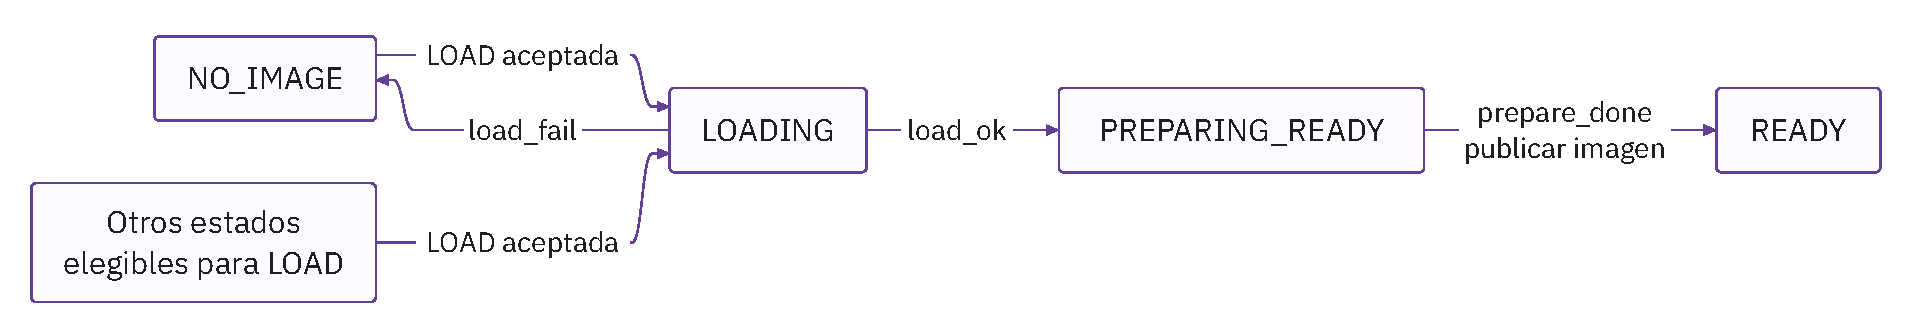
\includegraphics[width=0.94\textwidth]{fsm-carga.pdf}
  \caption{Carga y publicación de la imagen. Una carga fallida vuelve a
  \code{NO_IMAGE}; la preparación exitosa publica la imagen sin ejecutar CPU.}
  \label{fig:fsm-carga}
\end{figure}

\code{LOAD} es elegible en \code{NO_IMAGE}, \code{READY}, \code{STEPPING},
\code{HALT_DRAIN_STEP}, \code{FAULT_DRAIN_STEP}, \code{FINISHED} y
\code{FAULT}. Durante carga, preparación, ejecución continua o drenado
automático, una nueva solicitud de carga se rechaza y la actividad en curso
continúa según corresponda.

Una vez en \code{READY}, las órdenes \code{RUN} y \code{STEP} inician la
ejecución continua o paso a paso, respectivamente. La
figura~\ref{fig:fsm-ejecucion} también muestra qué sucede después de terminar:
la imagen puede reutilizarse, pero primero se prepara una sesión nueva para
que no herede el estado de la ejecución anterior.

\begin{figure}[H]
  \centering
  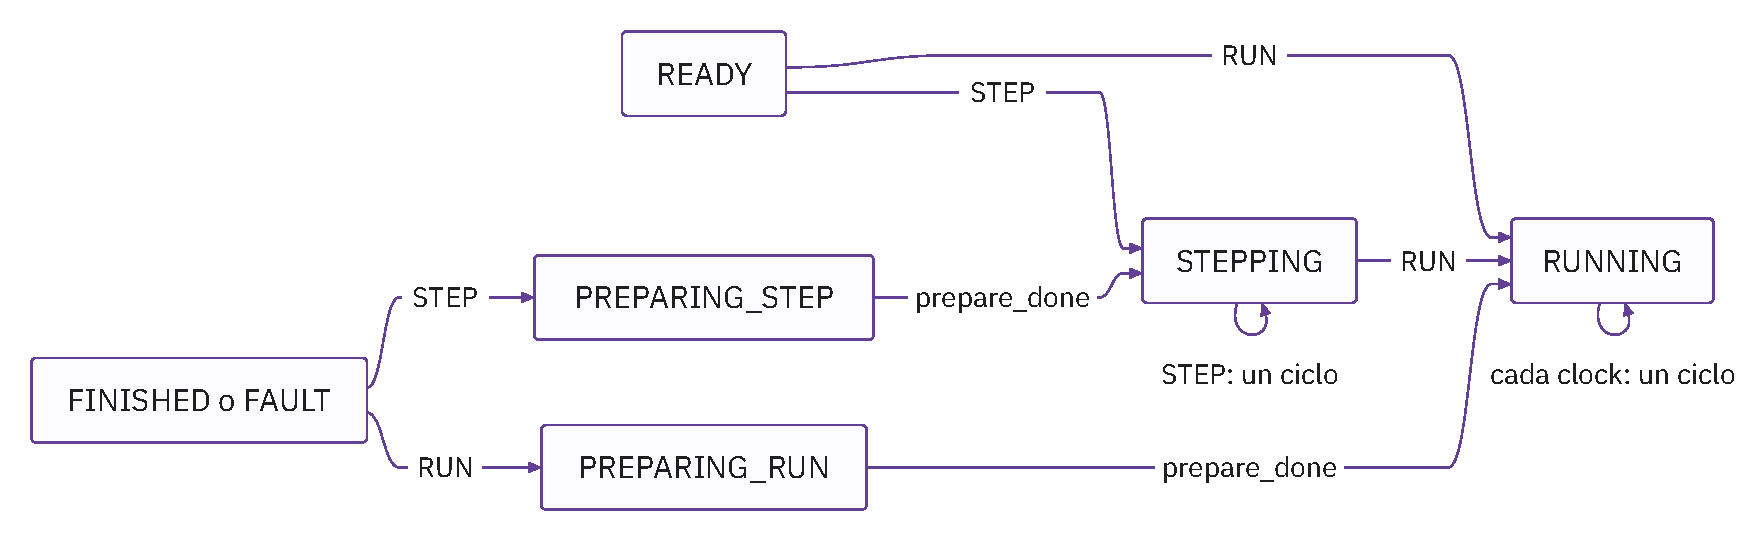
\includegraphics[width=\textwidth]{fsm-ejecucion.pdf}
  \caption{Inicio, reanudación y reutilización de una imagen. Las transiciones
  hacia \code{RUNNING} o \code{STEPPING} ejecutan el primer ciclo; desde un
  terminal, la orden espera a que termine la preparación.}
  \label{fig:fsm-ejecucion}
\end{figure}

Cuando se confirma \code{halt} o un fault, el pipeline puede conservar
instrucciones anteriores que deben completar sus efectos. La
figura~\ref{fig:fsm-drenado} muestra los estados que permiten terminar ese
trabajo. Si ya no queda ninguna instrucción anterior, el sistema pasa
directamente al estado terminal correspondiente.

\begin{figure}[H]
  \centering
  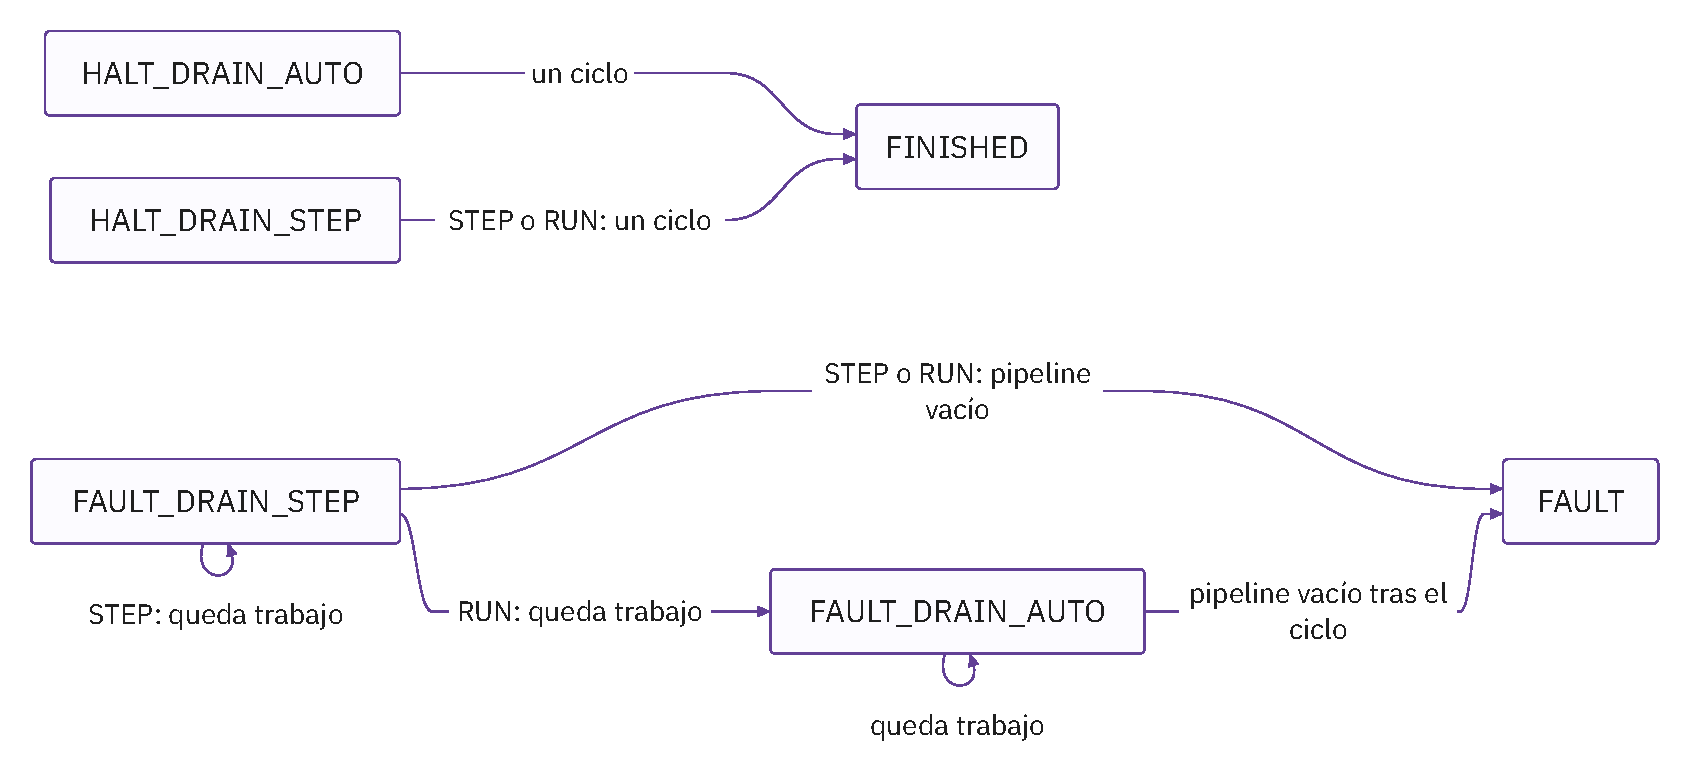
\includegraphics[width=\textwidth]{fsm-drenado.pdf}
  \caption{Drenado de instrucciones anteriores. El drenado por \code{halt}
  termina en un ciclo efectivo; el de fault puede requerir dos. En modo STEP,
  cada avance requiere autorización y RUN permite completar automáticamente.}
  \label{fig:fsm-drenado}
\end{figure}

\section{LOAD, RUN, STEP y RESET}

Las órdenes recibidas desde la PC permiten cargar una imagen y controlar su
ejecución. Cada una tiene un propósito diferente: \code{LOAD} incorpora un
programa, \code{RUN} y \code{STEP} determinan cómo avanza la CPU, y
\code{RESET} devuelve el sistema a su estado de reinicio.

\subsection{LOAD}

La carga comienza con una cabecera de seis bytes que contiene el código
\code{0x01} y el tamaño del programa, expresado como un entero sin signo de
cinco bytes en orden little-endian. La FPGA valida la solicitud antes de
aceptarla. Si es válida, responde \code{LOAD/ACCEPTED} y la PC envía los $N$
bytes anunciados. A medida que los recibe, el \code{Loader} forma palabras de
cuatro bytes y las escribe en IMEM.

Cuando se escribe la última palabra, \code{load_ok} indica que la recepción
terminó y la FSM pasa a \code{PREPARING_READY}. Allí se prepara el estado de
la primera sesión y, al finalizar, se publica la imagen y se responde
\code{LOAD/DONE}. La imagen anterior se invalida al aceptar la carga, por lo
que una transferencia parcial o fallida deja al sistema sin imagen ejecutable
hasta que se complete una carga posterior. El intercambio se detalla en
\doc{protocol.md}{Protocolo UART}.

\subsection{RUN}

\code{RUN} inicia o reanuda la ejecución continua. Si se acepta en
\code{READY}, el mismo flanco ejecuta el primer ciclo de la CPU, que realiza el
primer fetch con el pipeline vacío. A partir de entonces, en \code{RUNNING},
se solicitan ciclos automáticamente hasta que se confirme \code{halt} o un
fault.

La ejecución continua no implica ciclos idénticos: dentro de \code{RUNNING}
puede haber avance normal, stall \code{load-use}, redirect o confirmación de
\code{halt}/fault. Todos son ciclos efectivos. Un stall no detiene el modo
continuo; un redirect cambia el PC pero no abandona la sesión.

\subsection{STEP}

\code{STEP} permite observar la ejecución ciclo a ciclo. La CPU utiliza el
mismo datapath que en \code{RUN}, pero después de cada ciclo vuelve a esperar
una orden. Si se acepta en \code{READY}, el flanco de aceptación realiza el
primer fetch y la FSM pasa a \code{STEPPING}. Desde allí, otro \code{STEP}
autoriza un ciclo y \code{RUN} reanuda la ejecución continua.

Un paso corresponde a un ciclo de pipeline, no a la ejecución completa de una
instrucción. Por eso, en un mismo paso pueden avanzar varias instrucciones en
etapas diferentes.

Un stall \code{load-use} consume el \code{STEP}. Aunque el consumidor quede
retenido, el ciclo existió: el load y las instrucciones anteriores avanzaron. No
se ejecuta un segundo ciclo automático para completar la dependencia. Esta
distinción entre \code{STEP} y \code{HOLD} es fundamental para la observación y
se resume en la tabla~\ref{tab:step-hold}.

\begin{table}[H]
  \centering
  \small
  \begin{tabular}{lcc}
    \toprule
    \textbf{Situación} & \code{cpu_cycle_fire} & \textbf{Efecto} \\
    \midrule
    Stall \code{load-use} & 1 & parte del pipeline avanza; se consume un
    \code{STEP} \\
    \code{HOLD} & 0 & no hay avance de CPU ni consumo de \code{STEP} \\
    \bottomrule
  \end{tabular}
  \caption{Diferencia entre stall y \code{HOLD}.}
  \label{tab:step-hold}
\end{table}

\subsection{RESET}

El reset interrumpe la actividad vigente y tiene prioridad sobre los demás
efectos funcionales. Puede solicitarse mediante UART o con el botón físico de
la placa. Para el comando UART, el sistema transmite primero la respuesta
\code{RESET/ACCEPTED} completa, incluido el bit de Stop del último byte, y
después registra la solicitud de reset global. El botón físico puede actuar en
cualquier momento.

Al finalizar el reset, el sistema queda en \code{NO_IMAGE}, con PC, banco de
registros, contador, registros interetapa y tamaño confirmado en su estado
inicial. La imagen anterior deja de ser ejecutable y la preparación posterior
establece el cero lógico de DMEM. La secuencia temporal y las fuentes de reset
se detallan en \doc{architecture/platform/reset_integration.md}{Integración
del reset}.

\section{Preparación de una sesión}

La preparación establece un estado inicial limpio antes de ejecutar una
imagen. Se utiliza tanto después de una carga como cuando se vuelve a ejecutar
una imagen que ya terminó una sesión. En este último caso, las instrucciones
permanecen en IMEM y se restablece el estado de ejecución.

En el primer flanco de preparación se inicializan el PC, el banco de registros,
los registros interetapa y el contador, a la vez que se limpia la primera marca
de validez de DMEM. Los flancos siguientes limpian las demás marcas, una por
ciclo de reloj. Al terminar el recorrido, \code{prepare_done} indica que el
estado inicial está listo.

La FSM conserva el motivo de la preparación mediante tres estados. Aunque los
tres usan el mismo mecanismo, al finalizar entregan el control de manera
distinta:

\begin{itemize}
  \item \code{PREPARING_READY} prepara la primera sesión de una imagen recién
    cargada. Al terminar, publica la imagen y pasa a \code{READY}, donde espera
    una orden.
  \item \code{PREPARING_RUN} prepara una nueva ejecución continua de la imagen
    conservada. Al terminar, autoriza el primer ciclo y pasa a \code{RUNNING}.
  \item \code{PREPARING_STEP} prepara una nueva ejecución paso a paso. Al
    terminar, autoriza el primer ciclo y pasa a \code{STEPPING}.
\end{itemize}

La preparación completa dura 2049 ciclos de reloj en \code{REFERENCE} y 1001
en \code{ALT_1000}. A \SI{50}{\mega\hertz}, ambas duraciones caben en el
presupuesto de \SI{1}{\milli\second} para la preparación posterior a una carga.
Esos ciclos de preparación no incrementan el contador de la CPU.

\section{Drenado y terminación}

Una sesión termina normalmente al confirmar \code{halt} y termina de forma
excepcional al confirmar un fault. En cualquiera de los dos casos pueden quedar
en MEM o WB instrucciones anteriores que todavía deben completar sus efectos.
El drenado permite que esas instrucciones terminen mientras impide el ingreso
de trabajo nuevo. La instrucción que produjo el fault se descarta, \code{halt}
se consume en EX y las instrucciones posteriores también se descartan.

Si la confirmación ocurrió durante \code{RUN}, los estados
\code{HALT_DRAIN_AUTO} y \code{FAULT_DRAIN_AUTO} autorizan los ciclos restantes
automáticamente. Si ocurrió durante \code{STEP}, se entra en el estado de
drenado paso a paso correspondiente y cada \code{STEP} autoriza un ciclo más.
También puede solicitarse \code{RUN} para completar el drenado de forma
automática.

El control examina los indicadores de validez que tendrán los cuatro registros
interetapa después del ciclo. Cuando ya no queda trabajo, pasa a
\code{FINISHED} para una terminación normal o a \code{FAULT} para una
excepcional. Así, el último ciclo útil puede llevar directamente al estado
terminal sin agregar un ciclo vacío.

\section{Contador de ciclos}

El contador \code{cycle_count} permite conocer cuántos ciclos efectivos de CPU
transcurrieron durante la sesión. Es un valor sin signo de 64 bits que se pone
en cero durante la preparación y se incrementa una vez cada vez que se activa
\code{cpu_cycle_fire}.

El conteo incluye avances normales, stalls, redirects, confirmaciones de
\code{halt} o fault y ciclos de drenado. En cambio, durante \code{HOLD}, la
carga, la transmisión por UART, Debug y la preparación pueden transcurrir
ciclos del reloj físico sin que el contador avance.

Si alcanza \code{0xffffffffffffffff}, el incremento siguiente lo lleva a cero
sin generar un fault ni cambiar el modo de ejecución. Su valor completo se
incluye en el snapshot para relacionar el estado observado con los ciclos de la
sesión y compararlo con una simulación.

\section{Programas que no alcanzan \code{halt}}

Un programa puede ejecutar un bucle sin llegar a \code{halt}. En modo
\code{RUN}, si las instrucciones y sus accesos siguen siendo válidos, la CPU
continúa ejecutando sin un límite automático de ciclos.

Si el flujo intenta buscar una instrucción fuera de la imagen cargada, se
confirma un fault de acceso a instrucción. La sesión termina entonces en
\code{FAULT}, una vez completado el drenado que corresponda. Del mismo modo,
una instrucción ilegal produce un fault en lugar de una terminación normal.

En modo \code{STEP}, la CPU permanece detenida entre órdenes, aunque el
programa no tenga fin. Para interrumpir un \code{RUN} que no termina se utiliza
\code{RESET} por UART o el botón físico. Ambos invalidan la imagen y dejan el
sistema listo para recibir otra carga. Si una herramienta agota su tiempo de
espera, ese evento solo informa que dejó de esperar una respuesta; no significa
que la CPU haya terminado. Esta política corresponde a
\doc{decisions/DEC-SYS-002.md}{la decisión sobre ausencia de STOP/HALT}.

\section{Reprogramación}

Una imagen nueva puede reemplazar a la anterior sobre la misma configuración de
FPGA. Al aceptar \code{LOAD}, el sistema abandona la sesión vigente e invalida
el tamaño confirmado de la imagen anterior. Después de recibir la nueva imagen,
la preparación establece el estado inicial antes de publicarla.

La tabla~\ref{tab:reprogramacion} resume cómo participa cada elemento en este
proceso. En particular, el contenido físico de las memorias puede conservar
datos anteriores, pero el tamaño confirmado y las marcas de validez determinan
qué contenido pertenece a la nueva sesión.

\begin{table}[H]
  \centering
  \small
  \begin{tabularx}{\textwidth}{L{3.2cm}Y}
    \toprule
    \textbf{Elemento} & \textbf{Política} \\
    \midrule
    PC & Vuelve a cero en la preparación. \\
    IMEM & Conserva el array físico; la nueva imagen se escribe palabra por
    palabra. El tamaño confirmado delimita lo ejecutable. \\
    DMEM & Conserva el array físico; la preparación limpia las marcas de
    validez y el contenido no escrito se observa como cero. \\
    Banco de registros & Se inicializa en cero lógico durante la preparación. \\
    Registros interetapa & Se invalidan; los campos residuales no producen
    efectos. \\
    Debug & LOAD solo se acepta después de completar la respuesta anterior.
    Un snapshot de la sesión previa no representa el estado de la nueva. \\
    Control & La FSM inicia la carga y, si termina correctamente, prepara y
    publica la nueva imagen. Si la carga falla, queda en \code{NO_IMAGE}. \\
    \bottomrule
  \end{tabularx}
  \caption{Política de reprogramación.}
  \label{tab:reprogramacion}
\end{table}


\chapter{Hazards, forwarding y cambios de flujo}\label{chap:hazards}
En un procesador segmentado, varias instrucciones se encuentran en distintas
etapas al mismo tiempo. Esa superposición mejora el aprovechamiento del
pipeline, pero también exige coordinar instrucciones que comparten datos o que
pueden modificar el flujo de ejecución. En este capítulo se explican los
\emph{hazards} que aparecen en el diseño y los mecanismos que permiten resolverlos.

\section{Por qué aparecen hazards}

Una dependencia de datos aparece cuando una instrucción necesita el resultado
de otra que todavía está en el pipeline. Por ejemplo, una suma puede producir
un valor que la instrucción siguiente debe utilizar. Si esta última toma el
valor anterior del banco de registros, ejecuta la operación con un operando
incorrecto.

Para evitarlo, el procesador utiliza tres mecanismos según el momento en que el
resultado está disponible y la etapa que lo necesita:

\begin{itemize}
  \item \textbf{Forwarding hacia EX:} reenvía un resultado disponible desde
    \code{EX/MEM} o \code{MEM/WB} a la instrucción que lo necesita en EX.
  \item \textbf{Bypass \tech{WB}$\rightarrow$\tech{ID}:} entrega a ID el valor
    que WB está por escribir cuando ambas etapas acceden al mismo registro.
  \item \textbf{Espera \code{load-use}:} retrasa al consumidor inmediato de un
    load hasta que el dato leído de memoria está disponible para forwarding.
\end{itemize}

También pueden aparecer dependencias de control, por ejemplo cuando un branch
tomado cambia la dirección desde la que deben buscarse las instrucciones. La
tabla~\ref{tab:tipos-hazard} resume los casos considerados y cómo los trata el
diseño.

\begin{table}[H]
  \centering
  \small
  \begin{tabularx}{\textwidth}{L{3.0cm}L{3.6cm}Y}
    \toprule
    \textbf{Clase} & \textbf{Ejemplo} & \textbf{Tratamiento} \\
    \midrule
    Dato RAW & \code{add} seguido de un consumidor de su resultado &
    Forwarding desde \code{EX/MEM} o \code{MEM/WB}; bypass
    \tech{WB}$\rightarrow$\tech{ID} si el productor está en WB. \\
    \addlinespace
    Dato RAW con load & \code{lw} seguido de un consumidor inmediato &
    \code{load-use}: retener el consumidor e insertar una burbuja. \\
    \addlinespace
    Control & Branch tomado, \code{JAL} o \code{JALR} & Resolución en EX;
    redirect y descarte de las dos instrucciones jóvenes. \\
    \addlinespace
    Estructural & IF y MEM en el mismo ciclo & No existe: IMEM y DMEM son
    espacios independientes y permiten accesos simultáneos. \\
    \addlinespace
    WAW / WAR & Dos escrituras o una lectura y una escritura & No existen en un
    pipeline \emph{in-order} con escritura única en WB. \\
    \bottomrule
  \end{tabularx}
  \caption{Clases de hazard y su tratamiento.}
  \label{tab:tipos-hazard}
\end{table}

La especificación completa, con ecuaciones y prioridades, se encuentra en
\doc{architecture/cpu/control_and_hazards.md}{Control y hazards}.

\section{Forwarding hacia EX}

Cuando una instrucción llega a EX, los operandos que trajo desde ID pueden
haber quedado desactualizados: una instrucción anterior todavía puede tener el
resultado más reciente dentro del pipeline. El forwarding resuelve ese caso
sin esperar a que el resultado se escriba y vuelva a leerse del banco de
registros.

Para cada fuente que la instrucción utiliza, la unidad de forwarding compara
su número de registro con los destinos de las instrucciones que están en
\code{EX/MEM} y \code{MEM/WB}. Si encuentra un productor válido, selecciona
su resultado; en caso contrario, conserva el valor que llegó en \code{ID/EX}.

La comparación considera únicamente instrucciones válidas que escriben un
registro distinto de \code{x0}, y solo examina las fuentes que el consumidor
usa realmente. Si ambos registros interetapa contienen un productor del mismo
destino, se aplica la siguiente prioridad:

\begin{codebox}
EX/MEM > MEM/WB > valor base ID/EX
\end{codebox}

\code{EX/MEM} tiene prioridad porque contiene la instrucción productora más
reciente. La figura~\ref{fig:forwarding} muestra cómo los valores de ambos
registros interetapa llegan a los selectores de operandos de EX, junto con los
valores originales transportados por \code{ID/EX}.

\begin{figure}[H]
  \centering
  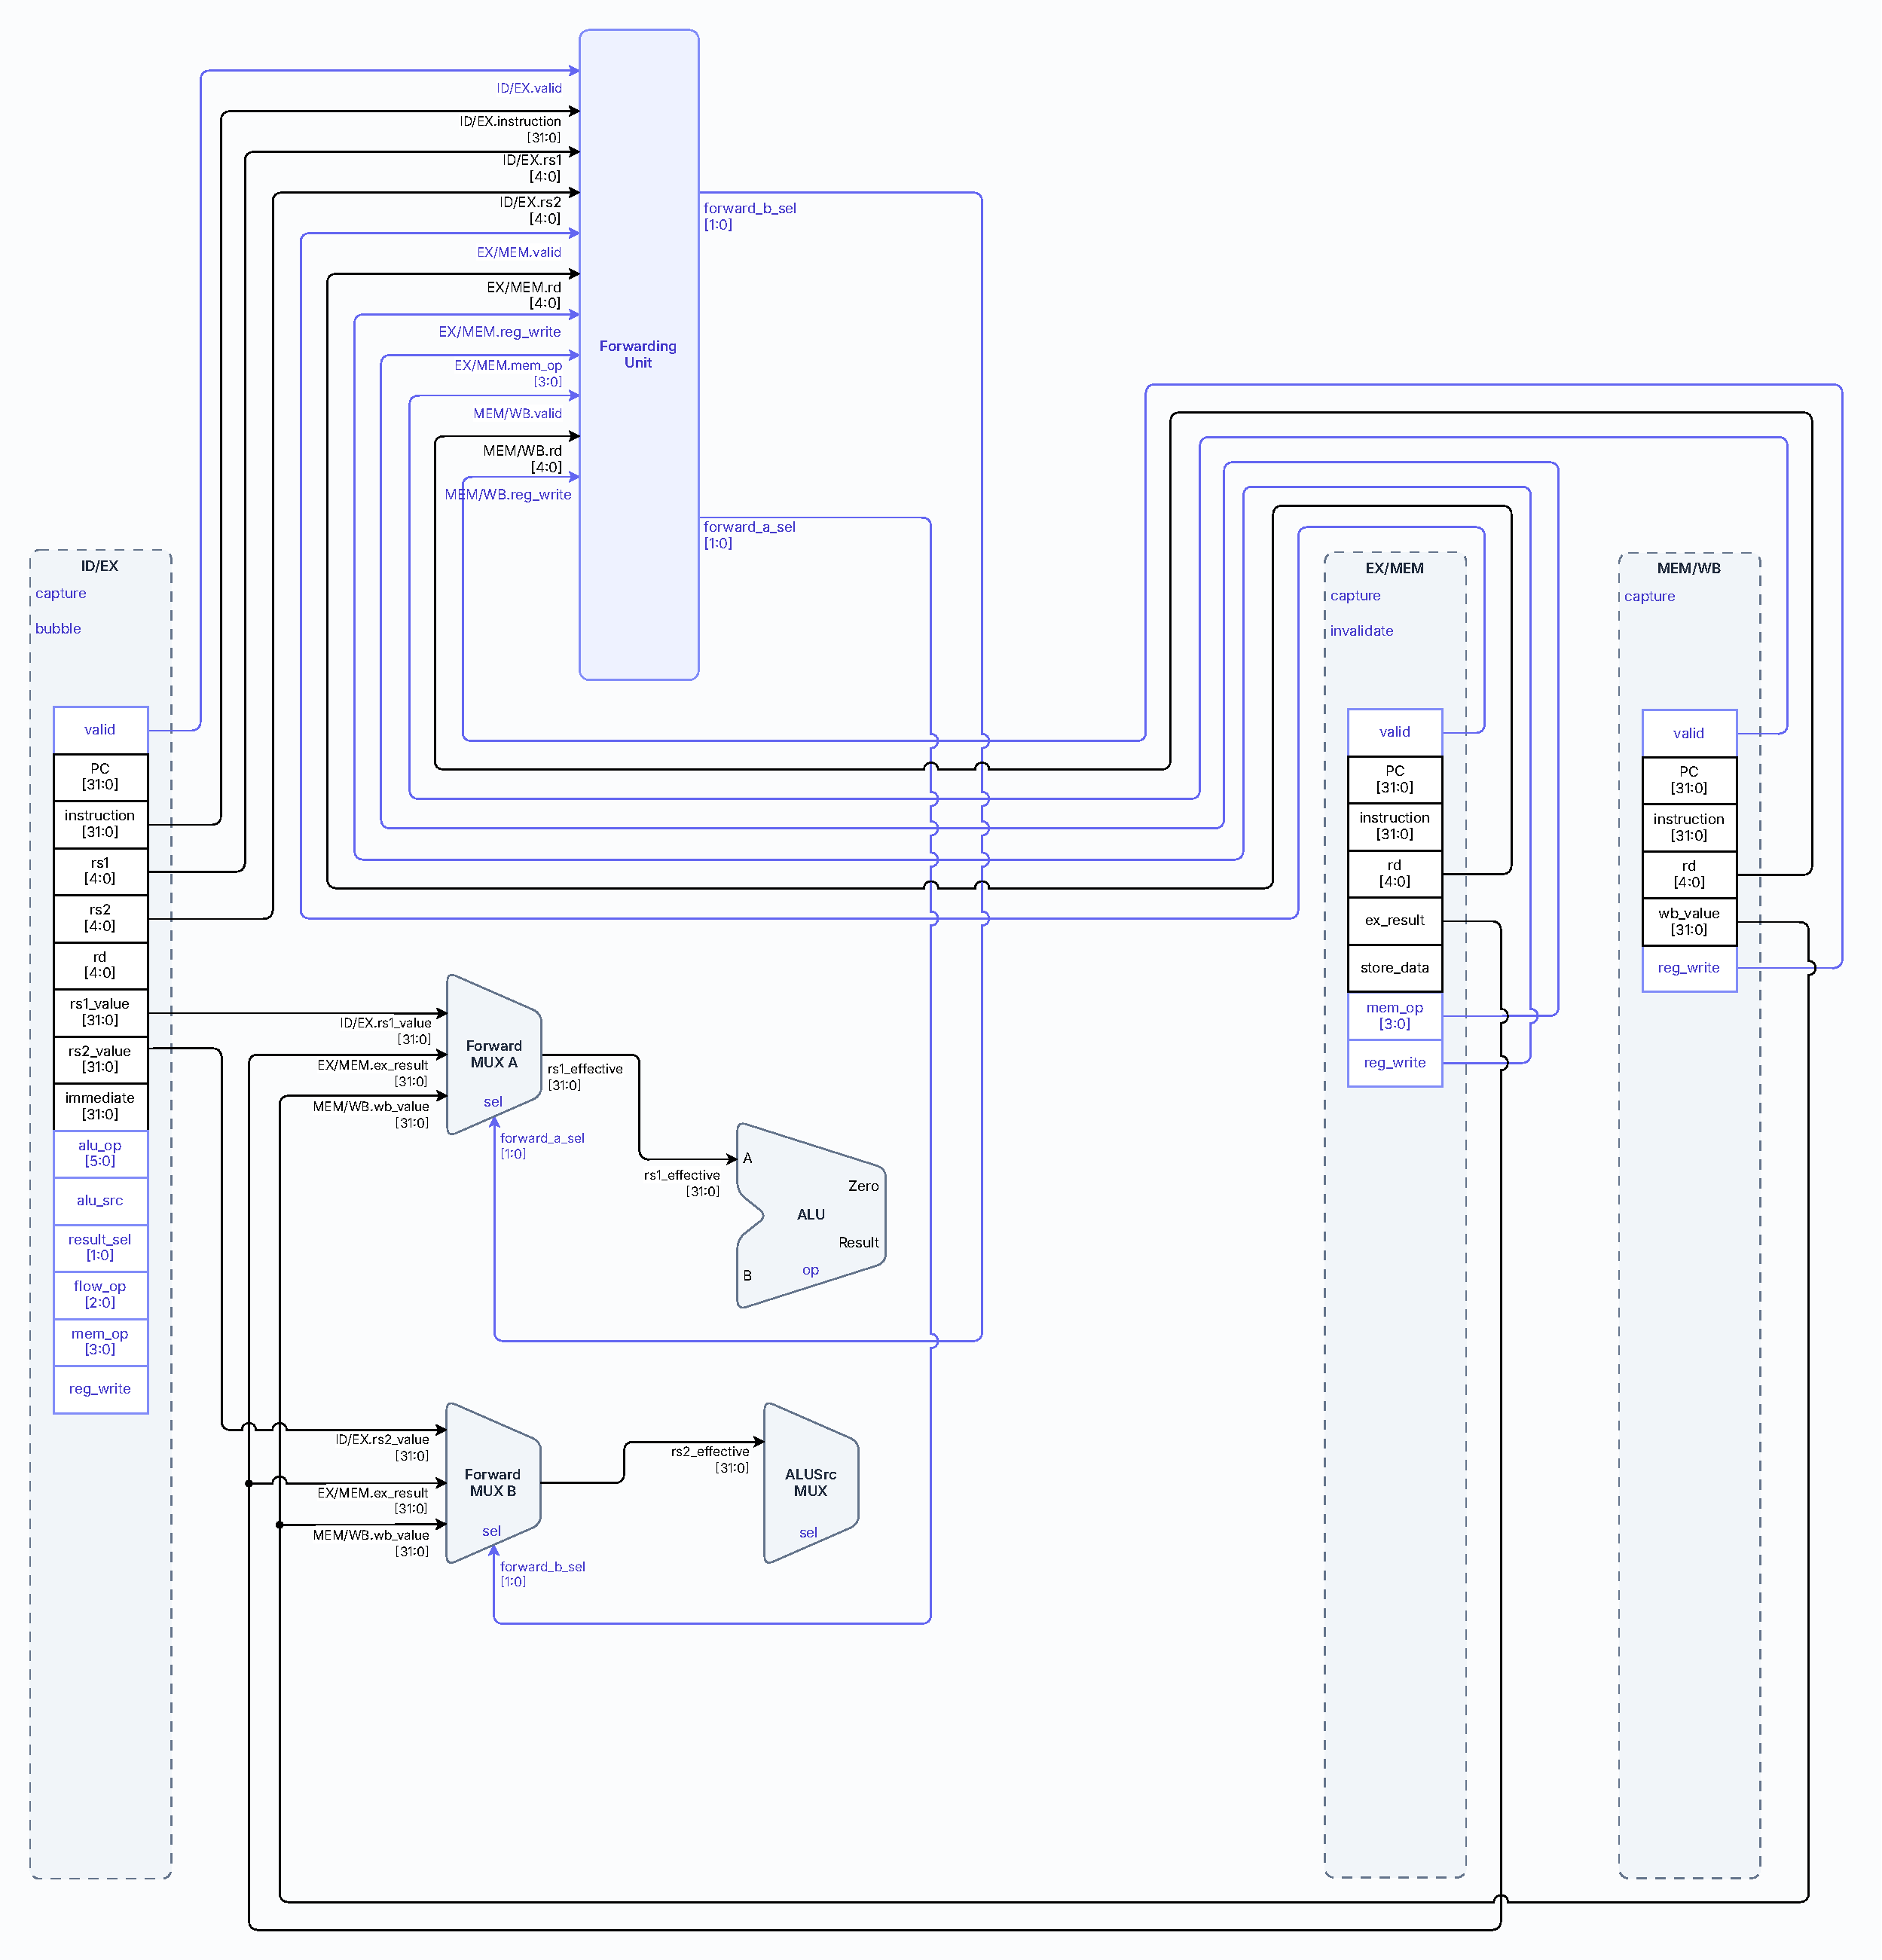
\includegraphics[width=0.95\textwidth,height=0.68\textheight,keepaspectratio]{forwarding.pdf}
  \caption{Recorrido del forwarding hacia los operandos de EX.}
  \label{fig:forwarding}
\end{figure}

\subsection{Ejemplo de forwarding desde \code{EX/MEM}}

Considérese la secuencia:

\begin{codebox}[language=RISCV]
add x1, x4, x5
sub x2, x1, x3
\end{codebox}

La tabla~\ref{tab:forwarding-exmem} muestra los ciclos relevantes. En C4, el
\code{add} está en MEM y el \code{sub} en EX; el resultado de \code{x1} todavía
no se escribió en el banco de registros, pero ya está en \code{EX/MEM}.
Forwarding selecciona ese valor y el \code{sub} opera con el dato correcto.

\begin{table}[H]
  \centering
  \small
  \begin{tabular}{clll}
    \toprule
    \textbf{Ciclo} & \textbf{\code{add}} & \textbf{\code{sub}} & \textbf{Acción} \\
    \midrule
    C3 & EX & ID & ID lee el valor base de \code{x1}. \\
    C4 & MEM & EX & Forwarding desde \code{EX/MEM} hacia la fuente 1. \\
    C5 & WB & MEM & WB escribe \code{x1}; el resultado de \code{sub} avanza. \\
    C6 & --- & WB & WB escribe \code{x2}. \\
    \bottomrule
  \end{tabular}
  \caption{Forwarding desde \code{EX/MEM} para el consumidor inmediato.}
  \label{tab:forwarding-exmem}
\end{table}

\subsection{El caso especial del load}

Un load requiere una consideración adicional. Al salir de EX, su resultado es
la dirección efectiva del acceso; el dato solicitado recién se obtiene en MEM.
Por lo tanto, la dirección que transporta \code{EX/MEM.ex_result} no puede
reenviarse como si fuera el valor que el load escribirá en el registro destino.

Si ese load es el productor más reciente, tampoco corresponde utilizar una
versión anterior del mismo registro desde \code{MEM/WB}. Las siguientes
condiciones expresan esa regla para cada fuente:

La condición de disponibilidad se expresa como:

\begin{codebox}
exmem_result_available = !is_load(EX/MEM.mem_op)
forward_exmem_rsN = exmem_match_rsN && exmem_result_available
forward_memwb_rsN = !exmem_match_rsN && memwb_match_rsN
\end{codebox}

La selección desde \code{MEM/WB} se bloquea cuando hay coincidencia con
\code{EX/MEM}, incluso si ese productor es un load cuyo dato aún no está
disponible. La espera \code{load-use}, explicada más adelante, evita que el
consumidor inmediato llegue a EX antes de tiempo.

\section{Bypass \texorpdfstring{WB$\rightarrow$ID}{WB a ID}}

El bypass entre WB e ID resuelve otra situación: una instrucción está por
escribir su resultado en el banco de registros mientras otra, en ID, lee ese
mismo registro. Como ambas operaciones coinciden en el ciclo, el valor leído
del banco podría no reflejar todavía la escritura.

Para que el consumidor reciba el resultado correcto, el bypass toma el valor
de WB y lo entrega directamente al puerto de lectura correspondiente. Así, el
comportamiento no depende del orden de lectura y escritura del banco en ese
flanco.

La selección se evalúa por separado para cada fuente y requiere que la escritura
de WB esté efectivamente habilitada:

\begin{codebox}
bypass_rs1 = rf_write_fire && (MEM/WB.rd == id_rs1)
bypass_rs2 = rf_write_fire && (MEM/WB.rd == id_rs2)
\end{codebox}

Cuando hay coincidencia, el puerto correspondiente selecciona
\code{MEM/WB.wb_value}; en caso contrario, conserva la lectura del banco. Los
valores seleccionados se capturan en \code{ID/EX} para que EX los utilice en el
ciclo siguiente. Si entonces existe un productor más reciente, el forwarding
de EX puede volver a reemplazarlos. La figura~\ref{fig:bypass} muestra estos
caminos desde WB y el banco de registros hasta los operandos de ID.

\begin{figure}[H]
  \centering
  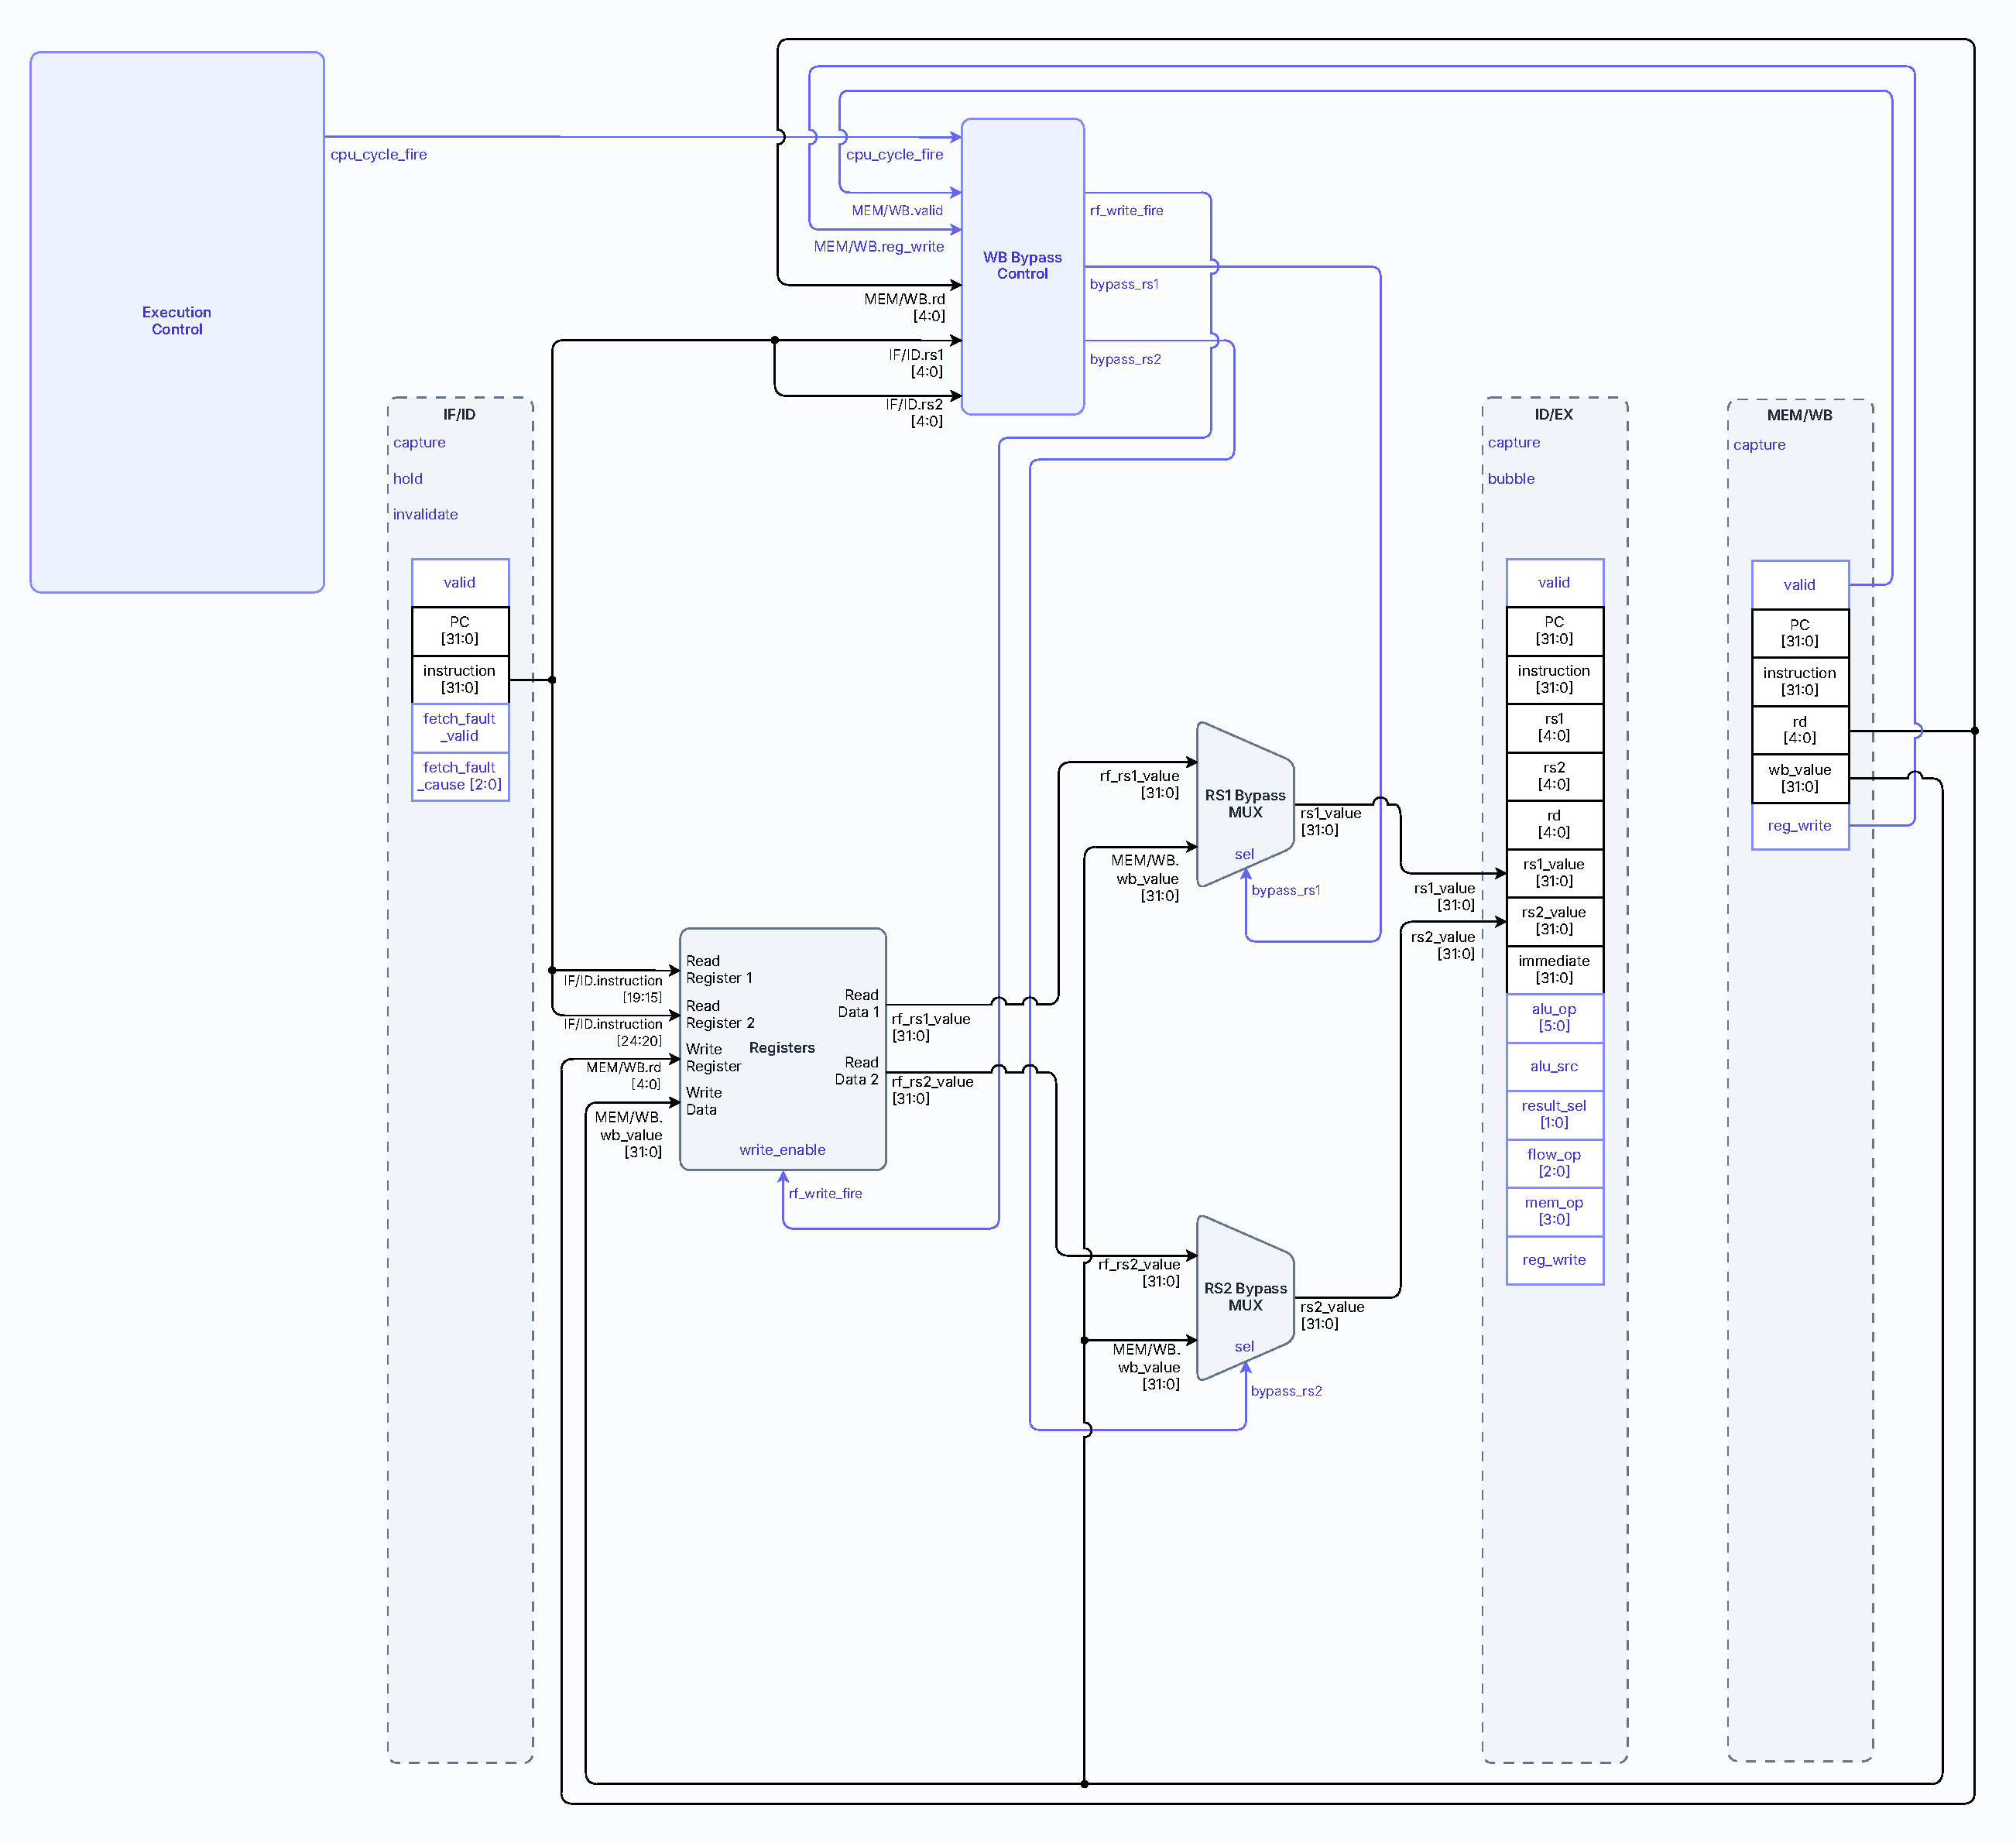
\includegraphics[width=0.95\textwidth,height=0.68\textheight,keepaspectratio]{bypass.pdf}
  \caption{Bypass \texorpdfstring{WB$\rightarrow$ID}{WB a ID}.}
  \label{fig:bypass}
\end{figure}

\section{Dependencia \texorpdfstring{load-use}{load-use}}

\subsection{Detección}

Una instrucción que utiliza inmediatamente el resultado de un load necesita una
espera. Cuando el load está en EX, calcula la dirección efectiva, pero el dato
se leerá en MEM durante el ciclo siguiente. Si ambas instrucciones avanzaran
sin demora, el consumidor llegaría a EX en ese mismo ciclo y necesitaría el
valor antes de que esté registrado en \code{MEM/WB}.

El diseño reenvía el resultado del load desde \code{MEM/WB}, por lo que retiene
al consumidor un ciclo para darle tiempo al load a completar la lectura.

Para reconocer esta dependencia, el detector compara el destino del load que
está en \code{ID/EX} con las fuentes utilizadas por la instrucción que espera
en \code{IF/ID}. La condición completa es:

\begin{codebox}
load_use_stall =
    ID/EX.valid
    && is_load(ID/EX.mem_op)
    && (ID/EX.rd != 0)
    && IF/ID.valid
    && (
         (ifid_uses_rs1 && (ifid_rs1 == ID/EX.rd))
         ||
         (ifid_uses_rs2 && (ifid_rs2 == ID/EX.rd))
       )
\end{codebox}

Una coincidencia accidental en un campo que la instrucción no usa no genera
dependencia. Tampoco participa un candidato de fetch, porque tiene
\code{IF/ID.valid = 0}. Un load con destino \code{x0} no crea dependencia.

\subsection{Efecto}

Cuando se selecciona la acción \code{act_load_use}, el control retiene la
instrucción consumidora e inserta una burbuja detrás del load. Las instrucciones
más antiguas continúan avanzando:

\begin{codebox}
PC       -> retener
IF/ID    -> retener
ID/EX    -> bubble
EX/MEM   -> capturar EX
MEM/WB   -> capturar MEM
\end{codebox}

Durante el stall, el load pasa de EX a MEM y el consumidor permanece en ID. En
el ciclo siguiente, el load completa la lectura y su resultado se captura en
\code{MEM/WB}, mientras el consumidor avanza a \code{ID/EX}. Un ciclo después,
el consumidor llega a EX y recibe por forwarding el dato ya registrado.

Aunque el consumidor permanezca detenido, el stall es un ciclo efectivo: el
contador aumenta, las instrucciones anteriores pueden completar sus efectos y,
en modo \code{STEP}, se consume una orden. En \code{HOLD}, en cambio, no se
autoriza un ciclo de CPU.

\section{Ejemplo ciclo a ciclo: \texorpdfstring{\code{TEST-PIPE-005/C001}}{TEST-PIPE-005/C001}}

El caso \code{TEST-PIPE-005/C001} del manifiesto ejecuta el siguiente programa
en \code{processor_top}:

\begin{codebox}[language=RISCV]
lw   x1, 0(x0)
add  x3, x1, x2
halt
\end{codebox}

El estado inicial prepara \code{x2 = 3} y \code{DMEM[0] = 8}. El resultado
esperado es \code{x1 = 8}, \code{x3 = 11}; el caso registra siete ciclos, un
stall, la escritura de \code{x1} en el ciclo 5, la de \code{x3} en el ciclo 7 y
la acción de load-use en el ciclo 3. La tabla~\ref{tab:load-use} muestra las
instrucciones presentes en cada etapa durante cada ciclo; a continuación se
explican las acciones que se producen al finalizar cada uno.

\begin{table}[H]
  \centering
  \small
  \begin{tabular}{lccccccc}
    \toprule
    \textbf{Ciclo} & \textbf{C1} & \textbf{C2} & \textbf{C3} & \textbf{C4} & \textbf{C5} & \textbf{C6} & \textbf{C7} \\
    \midrule
    \textbf{IF}  & \code{lw} & \code{add} & \code{halt} & \code{halt} & --- & --- & --- \\
    \textbf{ID}  & --- & \code{lw} & \code{add} & \code{add} & \code{halt} & --- & --- \\
    \textbf{EX}  & --- & --- & \code{lw} & Burbuja & \code{add} & \code{halt} & --- \\
    \textbf{MEM} & --- & --- & --- & \code{lw} & Burbuja & \code{add} & --- \\
    \textbf{WB}  & --- & --- & --- & --- & \code{lw} & --- & \code{add} \\
    \bottomrule
  \end{tabular}
  \caption{Recorrido del caso \code{TEST-PIPE-005/C001} por ciclo y por etapa.
  Cada columna muestra el estado durante el ciclo, antes del flanco que lo cierra.}
  \label{tab:load-use}
\end{table}

El recorrido se desarrolla de la siguiente manera:

\begin{description}
  \item[C1:] Se busca \code{lw}, se captura en \code{IF/ID} y el PC pasa a 4.
  \item[C2:] Se busca \code{add}, el \code{lw} avanza a EX y el PC pasa a 8.
  \item[C3:] Se detecta la dependencia mientras \code{lw} está en EX y
    \code{add} en ID. En el flanco que cierra el ciclo se retienen el PC y
    \code{IF/ID}, \code{lw} avanza a \code{EX/MEM} y se invalida
    \code{ID/EX}, insertando la burbuja.
  \item[C4:] La burbuja ocupa EX, mientras \code{lw} está en MEM y
    \code{add} sigue en ID. Al cerrar el ciclo se captura \code{halt},
    \code{add} avanza a EX y el dato leído por \code{lw} se captura en
    \code{MEM/WB}.
  \item[C5:] El forwarding entrega ese dato al \code{add}, que calcula
    \code{x3 = 11}, mientras WB escribe \code{x1 = 8}.
  \item[C6:] Se confirma \code{halt} en EX, se descarta el trabajo posterior y el
    \code{add} avanza hacia WB.
  \item[C7:] WB escribe \code{x3 = 11}; el pipeline queda vacío y la sesión pasa a
    \code{FINISHED}.
\end{description}

\section{Cambios de flujo y descarte}

\subsection{Saltos y branches}

El procesador busca instrucciones de manera secuencial mientras las anteriores
avanzan por el pipeline. Sin embargo, un branch tomado o un salto puede indicar
que la ejecución debe continuar en otra dirección. Como esa decisión se toma
en EX, para entonces ya pueden haberse buscado dos instrucciones posteriores:
una está en ID y la otra en IF.

Cuando se confirma el cambio de flujo, también llamado \emph{redirect}, el PC
recibe la dirección de destino y se descartan esas dos instrucciones, porque
pertenecen al camino que se abandonó. La instrucción que produjo el cambio y
las anteriores continúan avanzando. En \code{JAL} y \code{JALR}, esto permite
conservar el valor de enlace que luego se escribirá en el registro destino.

El descarte de las dos instrucciones produce una penalización de dos ciclos.
La ejecución continúa desde el nuevo PC y mantiene la modalidad elegida:
\code{RUN} sigue avanzando automáticamente, mientras que \code{STEP} espera la
siguiente orden.

\subsection{Faults y \code{halt}}

Cuando se confirma un fault o un \code{halt}, el procesador deja de admitir
instrucciones nuevas y descarta las que son posteriores al evento. Las
instrucciones anteriores, en cambio, pueden terminar sus efectos mediante el
drenado explicado en el capítulo anterior.

Si el fault se confirma en ID, la instrucción que está en EX es anterior y
puede avanzar. Si se confirma en EX, la instrucción que lo produjo se descarta
antes de llegar a MEM. Por su parte, \code{halt} se consume en EX y representa
una terminación normal.

\subsection{Selección de la acción del pipeline}

En cada ciclo efectivo, \code{Pipeline Hazard Control} decide cómo actualizar
el PC y los registros entre etapas. Por ejemplo, ante una dependencia
\code{load-use} retiene al consumidor, mientras que ante un redirect descarta
las instrucciones del camino anterior. La tabla~\ref{tab:acciones} resume
estas decisiones, incluidas las que se utilizan durante el drenado.

En la tabla, «Capt.» indica que el registro recibe la salida de la etapa
señalada y «Burbuja» representa una entrada inválida. Al invalidar \code{IF/ID}
se limpian tanto \code{valid} como \code{fetch_fault_valid}; en los demás
registros, la invalidez se indica con \code{valid=0}.

\begin{table}[H]
  \centering
  \footnotesize
  \setlength{\tabcolsep}{3pt}
  \begin{tabularx}{\textwidth}{L{3.75cm}ZZZZZ}
    \toprule
    \textbf{Acción} & \textbf{PC} & \textbf{IF/ID} & \textbf{ID/EX} &
    \textbf{EX/MEM} & \textbf{MEM/WB} \\
    \midrule
    Fault en EX & Retener & Invalidar & Burbuja & Invalidar & Capt. MEM \\
    \code{halt} en EX & Retener & Invalidar & Burbuja & Invalidar & Capt. MEM \\
    Redirect & Destino & Invalidar & Burbuja & Capt. EX & Capt. MEM \\
    Fault en ID & Retener & Invalidar & Burbuja & Capt. EX & Capt. MEM \\
    \code{load-use} & Retener & Retener & Burbuja & Capt. EX & Capt. MEM \\
    Avance normal & PC+4 & Capt. IF & Capt. ID & Capt. EX & Capt. MEM \\
    Drenado con \code{load-use} & Retener & Retener & Burbuja & Capt. EX & Capt. MEM \\
    Avance de drenado & Retener & Invalidar & Capt. ID & Capt. EX & Capt. MEM \\
    \bottomrule
  \end{tabularx}
  \caption{Efecto de las acciones sobre el PC y los registros interetapa.}
  \label{tab:acciones}
\end{table}

Si varios eventos ocurren en el mismo ciclo, se selecciona una sola acción. En
ejecución ordinaria, el control los considera en este orden:

\begin{enumerate}
  \item fault de la instrucción en EX;
  \item \code{halt} en EX;
  \item redirect resuelto en EX;
  \item fault de la instrucción en ID;
  \item dependencia \code{load-use}.
\end{enumerate}

Si no ocurre ninguno de ellos, el pipeline avanza normalmente. Este orden
permite atender primero los eventos de la instrucción más antigua: la que está
en EX precede en el programa a la que está en ID. Durante el drenado se
seleccionan las acciones propias de esa fase; la variante de drenado con
\code{load-use} se conserva en el control, aunque no aparece en un drenado
legal. Las condiciones completas se detallan en
\doc{architecture/cpu/control_and_hazards.md}{Control y hazards}.


\chapter{Flujo de programación y observación}\label{chap:flujo-software}
Este capítulo describe cómo se prepara un programa en la PC, cómo se envía a
la FPGA y de qué manera se observa el estado del procesador durante su
ejecución. En ese recorrido participan el assembler, la aplicación
\tech{viewrv} y el protocolo de comunicación sobre UART.

\section{Recorrido completo}

El punto de partida es un programa escrito en el lenguaje assembler del TP3.
El assembler traduce sus instrucciones a una imagen de bytes y conserva una
relación entre las direcciones de las instrucciones y las líneas del código
fuente. Con esa información, \tech{viewrv} puede cargar el programa y
relacionar lo que ocurre en el procesador con el texto que escribió el usuario.

La figura~\ref{fig:flujo-completo} muestra el recorrido completo: la PC
prepara y envía la imagen, la FPGA la almacena en IMEM y ejecuta el programa,
y la PC recibe las observaciones para presentarlas al usuario. Una vez
configurada la placa, pueden cargarse programas diferentes sobre el mismo
bitstream.

\begin{figure}[H]
  \centering
  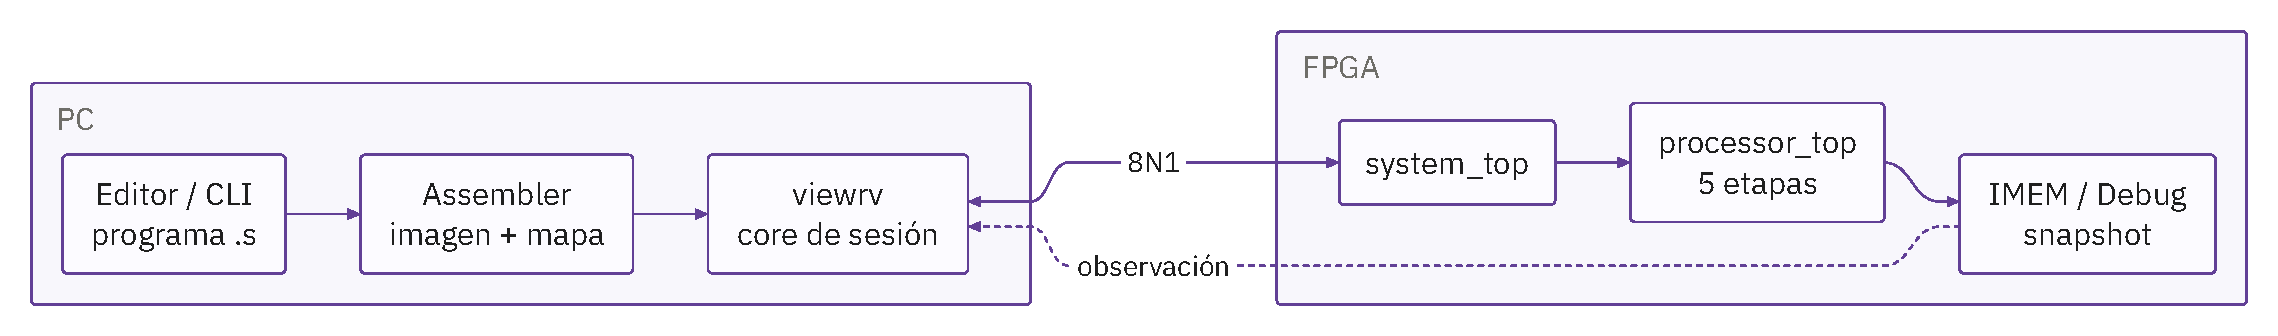
\includegraphics[width=\textwidth]{flujo-completo.pdf}
  \caption{Recorrido desde el programa assembler hasta la ejecución y la
  observación del procesador.}
  \label{fig:flujo-completo}
\end{figure}

\section{El assembler}

El assembler convierte el código fuente en las palabras de instrucción que
entiende el procesador. Cada instrucción ocupa cuatro bytes en orden
little-endian y se incorpora a una imagen continua que comienza en la dirección
cero. Además, el assembler genera un mapa que relaciona la dirección de cada
instrucción con su línea en el programa original.

La aplicación entrega el texto completo mediante la siguiente interfaz:

\begin{codebox}[language=Python]
assemble(source_text: str) -> AssemblyResult
\end{codebox}

El resultado reúne la imagen y el mapa cuando la traducción es correcta, o un
diagnóstico cuando encuentra un error:

\begin{itemize}
  \item \code{image}: los bytes de la imagen, o \code{None} si hubo un error;
  \item \code{pc_to_line}: la relación entre cada PC de instrucción y su línea
  fuente;
  \item \code{error}: un diagnóstico con línea y mensaje, o \code{None}.
\end{itemize}

Para traducir el programa, el assembler comprueba los mnemónicos, operandos,
registros, etiquetas y rangos de inmediatos admitidos por el lenguaje. El mapa
PC-línea queda en la aplicación, mientras que la imagen es el contenido que se
envía a la FPGA.

La traducción y la ejecución comprueban aspectos diferentes. El assembler
determina si el programa puede codificarse; después, la FPGA valida que la
imagen quepa en IMEM y el procesador comprueba las instrucciones y los accesos
durante la ejecución. Por eso, un ensamblado correcto no asegura por sí solo
que el programa termine normalmente.

El assembler está implementado en \code{tp3/software/assembler.py}. Su
interfaz, el lenguaje, la codificación y los diagnósticos se especifican en
\doc{software/assembler_interface.md}{la documentación del assembler}.

\section{\texorpdfstring{\tech{viewrv}}{viewrv}}

\tech{viewrv} es la aplicación local que permite preparar programas, controlar
la placa y observar el procesador. Ofrece una interfaz gráfica para trabajar
con el código y visualizar el pipeline, además de una interfaz de línea de
comandos para operar desde una terminal o automatizar recorridos.

Ambas interfaces utilizan un mismo \emph{core} local, que conserva la conexión
con la FPGA y coordina el estado de las sesiones. Así, la CLI puede realizar
varias operaciones sucesivas sin necesidad de mantener abierta la interfaz
gráfica. La comunicación con la placa utiliza el puerto serie y el protocolo
binario del TP3.

El trabajo de la aplicación se organiza en cuatro áreas:

\begin{itemize}
  \item \textbf{Programas y traducciones:} administra el código y sus
    versiones, invoca al assembler y vincula la imagen y el mapa PC-línea con
    el programa que los produjo.
  \item \textbf{Preparación y conexión:} coordina la programación del
    bitstream, identifica el puerto serie y establece el enlace con la placa.
  \item \textbf{Sesiones y resultados:} coordina la carga, la ejecución y la
    depuración, interpreta las capturas y administra los breakpoints.
  \item \textbf{Conservación:} guarda y recupera el código, las preferencias y
    los resultados de las sesiones.
\end{itemize}

La GUI utiliza Electron, React y TypeScript, mientras que el core y la CLI están
desarrollados en Python. Los clientes se comunican con el core mediante HTTP y
la GUI recibe actualizaciones de estado mediante SSE. La arquitectura y los
contratos se detallan en \doc{software/viewrv/arquitectura.md}{Arquitectura de
viewrv} y en \doc{software/viewrv/contratos.md}{Contratos de funcionamiento}.

\section{El protocolo sobre UART}

La comunicación entre la PC y la FPGA se realiza mediante un protocolo binario
sobre UART. La PC envía comandos para cargar o ejecutar un programa, y la FPGA
responde con el resultado de cada operación y, cuando corresponde, con el
estado observado del procesador.

\subsection{Enlace físico}

La conexión utiliza el puente USB-UART de la \tech{Basys 3}, a través del
conector micro-USB J4. La PC ve un puerto serie, mientras que la FPGA transmite
y recibe los datos mediante su módulo UART. El enlace se configura de la
siguiente manera:

\begin{itemize}
  \item \num{19200} baud nominales;
  \item 8 bits de datos, sin paridad, 1 bit de Start y 1 bit de Stop (8N1);
  \item sobremuestreo por 16 en el receptor de la FPGA;
  \item FIFO independientes de cuatro bytes para recepción y transmisión;
  \item un reloj funcional de \SI{50}{\mega\hertz} en la FPGA.
\end{itemize}

Con esta configuración, cada byte se transmite junto con un bit de inicio y
uno de parada. Por lo tanto, ocupa diez bits en el enlace y tarda
aproximadamente \SI{0.5208}{\milli\second} a \num{19200} baud.

Los mensajes se interpretan según la operación, que determina el orden y la
longitud de sus campos. El protocolo no agrega un marcador de fin, checksum ni
CRC.

\subsection{Comandos}

Cada solicitud comienza con un byte que identifica la operación. En el caso de
\code{LOAD}, también se envía el tamaño y, después de recibir la aceptación,
el contenido del programa. La tabla~\ref{tab:comandos} resume las solicitudes
disponibles.

Los campos de más de un byte usan orden little-endian. Los tamaños y las
cantidades se representan con cinco bytes sin signo para poder incluir el valor
$2^{32}$.

\begin{table}[H]
  \centering
  \small
  \begin{tabular}{cll}
    \toprule
    \textbf{Código} & \textbf{Operación} & \textbf{Solicitud} \\
    \midrule
    \code{0x01} & \code{LOAD} & Código + tamaño de cinco bytes; luego
    exactamente $N$ bytes de contenido. \\
    \code{0x02} & \code{RUN} & Un byte. \\
    \code{0x03} & \code{STEP} & Un byte. \\
    \code{0x04} & \code{RESET} & Un byte. \\
    \code{0x05} & \code{CHECK_READY} & Un byte. \\
    \bottomrule
  \end{tabular}
  \caption{Comandos del protocolo.}
  \label{tab:comandos}
\end{table}

Cada respuesta comienza con dos bytes: el código de la operación y un resultado
que indica, por ejemplo, si fue aceptada, si terminó o si se produjo un error.
Algunas respuestas incluyen datos adicionales, como el snapshot que acompaña
la ejecución. Los resultados y sus códigos se detallan en
\doc{protocol.md}{Protocolo UART}.

\subsection{Secuencia de carga}

La figura~\ref{fig:secuencia-load} muestra el intercambio de una carga normal.
Primero, la PC consulta si el sistema está disponible mediante
\code{CHECK_READY}. Luego envía la cabecera de \code{LOAD} con el tamaño de la
imagen y espera la respuesta de la FPGA antes de transmitir sus bytes.

La FPGA comprueba el tamaño antes de aceptar la carga. Después de recibir el
contenido y escribirlo en IMEM, prepara el estado de la sesión y publica la
imagen; recién entonces comunica que la operación terminó. Esta separación
permite distinguir la aceptación de la solicitud de la disponibilidad del
programa para ejecutar.

\begin{figure}[H]
  \centering
  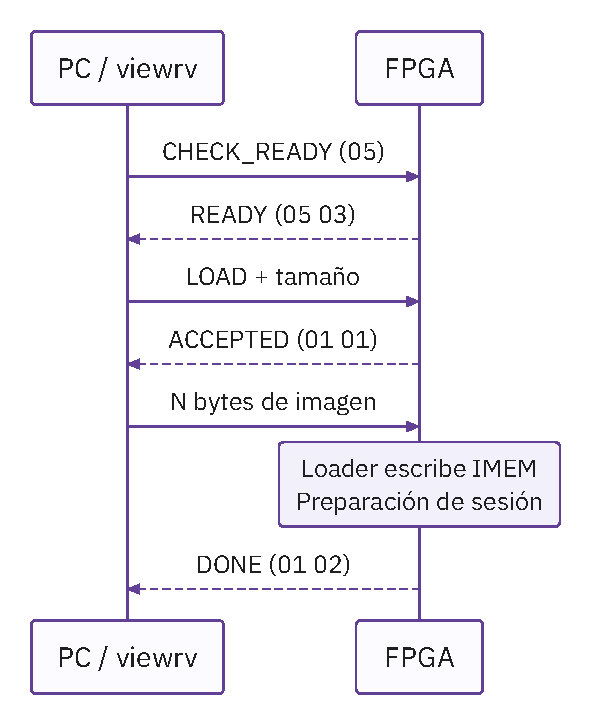
\includegraphics[width=0.42\textwidth]{secuencia-load.pdf}
  \caption{Secuencia normal de \code{LOAD}.}
  \label{fig:secuencia-load}
\end{figure}

\subsection{Secuencia de ejecución y observación}

Una vez cargada la imagen, la PC puede solicitar ejecución continua con
\code{RUN} o avanzar un ciclo con \code{STEP}. Un \code{RUN} aceptado recibe
primero \code{RUN/ACCEPTED}; cuando la sesión termina, la FPGA envía
\code{RUN/FINISHED} o \code{RUN/FAULT} junto con el snapshot final.

Cada \code{STEP} aceptado devuelve \code{STEP/DONE} y un snapshot posterior al
ciclo ejecutado. Durante la transmisión, la FPGA retiene el estado observado,
de modo que la respuesta describe un mismo instante de la sesión.

La tabla~\ref{tab:snapshot} muestra los campos del snapshot. Sus offsets se
cuentan desde el inicio del cuerpo, que sigue a la cabecera de dos bytes. El
cuerpo fijo ocupa 228 bytes y contiene, entre otros datos, el PC, los registros
arquitectónicos y el contenido de los registros interetapa.

Al final se agrega una entrada de cinco bytes por cada byte de DMEM escrito
durante la sesión: cuatro para la dirección y uno para el valor. Si $K$ es la
cantidad de entradas, la respuesta completa ocupa $230 + 5K$ bytes, incluida
la cabecera.

\begin{table}[H]
  \centering
  \small
  \begin{tabular}{lrl}
    \toprule
    \textbf{Campo} & \textbf{Offset} & \textbf{Bytes} \\
    \midrule
    \code{global_state} & 0 & 1 \\
    \code{image_valid} & 1 & 1 \\
    PC global & 2 & 4 \\
    \code{cycle_count} & 6 & 8 \\
    \code{fault_cause} & 14 & 1 \\
    \code{fault_pc} & 15 & 4 \\
    RF \code{x0..x31} & 19 & 128 \\
    \code{IF/ID} & 147 & 11 \\
    \code{ID/EX} & 158 & 30 \\
    \code{EX/MEM} & 188 & 20 \\
    \code{MEM/WB} & 208 & 15 \\
    \code{used_count} & 223 & 5 \\
    Lista de memoria & 228 & $5K$ \\
    \bottomrule
  \end{tabular}
  \caption{Estructura del snapshot de Debug. Los offsets del cuerpo se cuentan
  después de la cabecera de dos bytes.}
  \label{tab:snapshot}
\end{table}

\section{Cómo se observa el estado}

El snapshot permite examinar el estado del procesador después de un ciclo o al
finalizar una ejecución. Para construirlo, el serializador de la FPGA lee los
registros y la memoria definidos por el protocolo, mientras el estado de la
sesión permanece retenido. La aplicación recibe esos bytes y reconstruye:

\begin{itemize}
  \item el estado global de la sesión y la validez de la imagen;
  \item el PC y el contador de ciclos;
  \item la causa y el PC de fault, cuando corresponde;
  \item los 32 registros del banco;
  \item los 34 campos de los cuatro registros interetapa;
  \item la cantidad y la lista de bytes de DMEM escritos en la sesión.
\end{itemize}

Con esos datos, la GUI puede mostrar los registros, el contenido del pipeline,
la memoria utilizada y la línea de código asociada a una instrucción. La CLI
accede a la misma información y puede conservar los resultados en JSONL. El
mapa generado por el assembler permite relacionar los PC observados con el
código fuente de la imagen cargada.

Durante la depuración, la aplicación puede solicitar pasos sucesivos y examinar
cada snapshot para detectar coincidencias con los breakpoints configurados. La
observación corresponde a los datos recibidos de la FPGA; la aplicación
distingue esos datos de las interpretaciones que presenta al usuario.

Para que todos sus campos correspondan al mismo estado, la FPGA no admite otro
ciclo de CPU, una carga ni una preparación mientras se transmite el snapshot.
Si la respuesta se interrumpe, la PC descarta la captura parcial y conserva la
última que recibió completa, identificándola como anterior. La semántica
completa se consulta en
\doc{architecture/debug/debug_architecture.md}{Arquitectura de Debug} y en
\doc{protocol.md}{Protocolo UART}.


\chapter{Verificación funcional}\label{chap:verificacion}
La verificación busca comprobar que el procesador y los componentes que lo
rodean se comporten como se especificó. Para ello se prepararon casos con
entradas y resultados esperados, que se aplicaron tanto a bloques aislados como
a conjuntos cada vez más completos. Este capítulo presenta cómo se organizaron
esas pruebas, qué se comprobó y cuáles fueron los resultados registrados.

\section{Niveles de verificación}

Una prueba puede concentrarse en un bloque particular o examinar la interacción
entre varios componentes. Los niveles permiten distinguir qué parte del
sistema se observó en cada caso:

\begin{itemize}
  \item \textbf{Modelo abstracto:} comprueba reglas de control, recuperación y
    límites mediante un modelo de su comportamiento.
  \item \textbf{Unidad:} ejercita un bloque o una lógica local de manera
    aislada, como el detector de una dependencia.
  \item \textbf{Integración local:} comprueba una etapa o la conexión entre
    varios bloques, como el decoder junto con el detector.
  \item \textbf{CPU:} ejecuta programas sobre \code{processor_top} para
    observar el funcionamiento conjunto del procesador.
  \item \textbf{Sistema:} conecta la CPU con UART, el controlador de protocolo
    y el serializador para comprobar los intercambios y sus efectos.
  \item \textbf{Cliente PC:} comprueba la aplicación y su transporte, incluidos
    el tratamiento de respuestas y los tiempos de espera.
  \item \textbf{Elaboración y revisión:} examina tipos, parámetros, interfaces
    y dependencias de la implementación.
  \item \textbf{Implementación:} utiliza Vivado y los reportes del diseño
    físico para el perfil \code{REFERENCE}.
  \item \textbf{Placa:} ejecuta pruebas en la Basys 3 y compara las respuestas
    recibidas por UART.
\end{itemize}

Estos niveles se complementan. Por ejemplo, una prueba unitaria del detector
puede comprobar que reconozca una dependencia, pero hace falta observar la CPU
para verificar cómo se retiene y avanza el pipeline. Del mismo modo, una
simulación de CPU no comprueba por sí sola la comunicación física con la placa.

Para interpretar cada resultado se registra el caso y el nivel utilizado, junto
con el estímulo, la expectativa, lo observado y las herramientas
pertinentes. Si un banco agota su tiempo de espera, se informa como problema o
limitación de esa prueba, no como una terminación \code{FINISHED} de la CPU.

\section{Manifiesto y cobertura}

Las pruebas se organizan en un manifiesto: un catálogo que identifica qué se
comprueba, con qué entradas y cuál es el resultado esperado. Una especificación
puede tener varias variantes, por ejemplo distintos operandos o direcciones
límite. Cada grupo y cada variante tienen un identificador que permite localizar
su definición y sus resultados.

El manifiesto contiene 66 grupos y 1484 casos. La
tabla~\ref{tab:manifiesto} muestra cuántos corresponden a cada área y cuántos
figuran como implementados en el ejecutor de pruebas.

\begin{table}[H]
  \centering
  \small
  \begin{tabular}{lrrrr}
    \toprule
    \textbf{Área} & \textbf{Grupos} & \textbf{Casos} & \textbf{Implementados} &
    \textbf{No implementados} \\
    \midrule
    ISA & 8 & 537 & 537 & 0 \\
    Pipeline & 17 & 249 & 249 & 0 \\
    Memoria & 10 & 200 & 199 & 1 \\
    Ejecución & 11 & 222 & 222 & 0 \\
    UART y Debug & 14 & 248 & 248 & 0 \\
    Plataforma & 6 & 28 & 25 & 3 \\
    \midrule
    Total & 66 & 1484 & 1480 & 4 \\
    \bottomrule
  \end{tabular}
  \caption{Estado de los casos del manifiesto por área.}
  \label{tab:manifiesto}
\end{table}

Un caso definido describe una situación que se quiere comprobar; una ejecución
es un intento concreto de comprobarla con un banco y un nivel determinados. El
manifiesto registra 208 configuraciones de ejecución y un mismo caso puede
utilizarse en varias de ellas, por lo que la cantidad de ejecuciones de una
campaña puede superar la cantidad de casos. Además, que un caso esté
implementado indica que existe una prueba disponible, no que haya aprobado una
corrida.

La matriz de cobertura relaciona cada requisito con su contrato y sus pruebas:
\doc{verification/coverage.md}{la matriz de cobertura}.

Los cuatro casos que el ejecutor de simulación enumera como no implementados son
\code{TEST-MEM-008/C007}, \code{TEST-PLAT-003/C001},
\code{TEST-PLAT-004/C001} y \code{TEST-PLAT-006/C001}. Sus comprobaciones se
realizan mediante otras evidencias: revisión del formato de \code{LOAD},
elaboración y revisión estructural, implementación física y revisión documental,
respectivamente. Por eso se presentan por separado de las simulaciones.

\section{Verificación funcional}

La verificación funcional comprueba tanto los resultados de las instrucciones
como el comportamiento del pipeline, las memorias y el control de sesión. Por
ejemplo, se prueban operaciones aritméticas, codificaciones del decoder,
dependencias entre instrucciones y accesos a los límites de DMEM.

Las pruebas se agrupan según el aspecto del procesador que se quiere comprobar:

\begin{itemize}
  \item \textbf{Instrucciones:} se comprueban las operaciones aritméticas y
    lógicas, la formación de inmediatos y la identificación de instrucciones
    válidas e inválidas.
  \item \textbf{Pipeline:} se observan el avance de las instrucciones, el
    forwarding, las esperas por dependencias y el descarte ante cambios de flujo.
  \item \textbf{Memorias:} se verifican los tamaños de load y store, el orden
    de los bytes, la alineación y los límites de las direcciones.
  \item \textbf{Control de ejecución:} se comprueban la preparación, los
    modos RUN y STEP, el drenado y la respuesta ante \code{halt} o faults.
\end{itemize}

Por ejemplo, el caso de \emph{load-use} presentado en el capítulo 7 comprueba
una dependencia entre un load y la instrucción siguiente. El resultado esperado
incluye tanto el valor calculado como la espera necesaria para obtenerlo. El
detalle de este y de los demás casos se encuentra en el
\doc{verification/cases.json}{manifiesto de pruebas}.

\section{Resultados de la campaña}

Una vez preparadas las pruebas, se ejecutaron simulaciones de los bloques y del
sistema completo. También se probaron programas en la placa para comprobar el
recorrido real entre la PC y la FPGA. Los resultados de la simulación y de la
placa se presentan por separado porque cada uno observa condiciones distintas.

\subsection{Regresión de simulación RTL}

La \emph{regresión} consiste en volver a ejecutar un conjunto de pruebas para
comprobar que el diseño siga cumpliendo los resultados esperados. En la corrida
general se simularon las descripciones del hardware con Icarus Verilog y
Verilator. Se realizaron 2695 ejecuciones de simulación RTL: en la primera
corrida aprobaron 2692 y las tres restantes aprobaron al repetirse.

Además de las simulaciones, se comprobaron aspectos del código y de la
infraestructura de pruebas, y se ejecutaron las 114 pruebas del assembler.
Estas comprobaciones resultaron conformes.

\subsection{Pruebas de UART y Debug}

Las pruebas de integración comprueban el intercambio entre la CPU, el
controlador de protocolo, UART y Debug. Entre los escenarios ejercitados se
encuentran la carga de programas, la transmisión de memoria utilizada y el
comportamiento del reset.

Se realizaron pruebas dirigidas de estos intercambios con la CPU y los bloques
de comunicación conectados. También se simuló la integración con los componentes
de la plataforma para observar la comunicación y el reset. El procedimiento y
los resultados se desarrollan en el capítulo~\ref{chap:integracion-sistema}.

\subsection{Validación en placa}

La validación en placa permite comprobar el recorrido completo con la FPGA y la
comunicación UART reales. Para ello se cargaron programas, se controló su
ejecución desde la PC y se compararon las respuestas con los resultados
esperados. El procedimiento, los resultados y las pruebas que quedaron fuera de
su alcance se describen en el capítulo~\ref{chap:aceptacion-fisica}.

Las instrucciones para ejecutar las pruebas se encuentran en la
\doc{verification/test_selection.md}{guía de ejecución y selección de pruebas}.


\chapter{Integración de UART, Debug y CPU}\label{chap:integracion-sistema}
La integración conecta el procesador con los bloques que permiten cargar
programas, controlar su ejecución y consultar su estado desde una PC. Este
capítulo describe cómo colaboran esos bloques y qué pruebas comprueban su
funcionamiento en conjunto.

\section{Composición del sistema}

El sistema funcional está formado por cuatro bloques principales: la UART, el
controlador de protocolo, el serializador de respuestas y el procesador. La
tabla~\ref{tab:bloques-sistema} presenta la función de cada uno dentro del
recorrido de una solicitud.

El módulo \code{system_top} conecta estos bloques entre sí. A su vez,
\code{basys3_top} adapta el sistema a la placa: conecta sus pines, genera el
reloj de funcionamiento y acondiciona la señal de reset.

\begin{table}[H]
  \centering
  \small
  \begin{tabularx}{\textwidth}{L{4.4cm}Y}
    \toprule
    \textbf{Bloque} & \textbf{Función en la integración} \\
    \midrule
    \code{uart_core} & Sincroniza RX, genera el tick de baudios, recibe y
    transmite bytes y conserva las FIFO de recepción y transmisión. \\
    \addlinespace
    \code{protocol_controller} & Interpreta \code{LOAD}, \code{RUN},
    \code{STEP}, \code{RESET} y \code{CHECK_READY}; coordina las solicitudes,
    los tiempos de espera y la observación. \\
    \addlinespace
    \code{response_serializer} & Captura el descriptor de respuesta y produce
    la cabecera, el contexto, el banco de registros, los latches y la lista de
    DMEM en el orden aprobado. \\
    \addlinespace
    \code{processor_top} & Ejecuta la imagen y entrega el estado observable:
    PC, contador, RF, latches y metadatos de fault. \\
    \bottomrule
  \end{tabularx}
  \caption{Bloques de la integración de sistema.}
  \label{tab:bloques-sistema}
\end{table}

En un intercambio, la UART recibe los bytes de la PC y los entrega al
controlador. Este interpreta la solicitud y la coordina con el procesador;
después, el serializador forma la respuesta y la UART la transmite de vuelta.
El controlador atiende una operación normal por vez y, durante Debug, mantiene
estable el estado que se está enviando hasta que termina la respuesta.

\section{Coordinación de comandos y observación}

\subsection{LOAD y preparación}

La PC inicia \code{LOAD} enviando una cabecera de seis bytes que incluye el
tamaño del programa. El controlador valida ese tamaño y solicita al control
de ejecución que acepte la carga. Una vez recibida la respuesta
\code{ACCEPTED}, la PC transmite el contenido y el cargador del procesador
reconstruye las palabras para escribirlas en IMEM.

Cuando se recibe la última palabra, comienza la preparación del estado
inicial: se inicializan el PC, el banco de registros, los registros interetapa
y el contador, y se limpian las marcas de validez de DMEM. Al terminar la
preparación se publica la imagen y el sistema responde \code{DONE}, indicando
que el programa está disponible para ejecutar.

\subsection{RUN, STEP y Debug}

Una solicitud \code{RUN} aceptada inicia la ejecución continua y recibe una
respuesta \code{ACCEPTED}. Cuando el programa termina por \code{halt} o por un
fault y finaliza el drenado, la FPGA envía \code{FINISHED} o \code{FAULT} junto
con el snapshot del estado final. En cambio, \code{STEP} ejecuta un ciclo
efectivo y responde \code{DONE} con el estado posterior a ese ciclo.

Para construir el snapshot, el serializador consulta el estado que el
procesador expone para Debug y recorre el banco de registros y DMEM mediante
sus caminos de lectura compartidos. Mientras se transmite la respuesta, el
controlador mantiene retenida la CPU y excluye nuevas operaciones que podrían
modificar ese estado. Así, todos los campos enviados corresponden a la misma
observación, hasta que se transmite el bit de parada del último byte.

\section{Comprobaciones de integración}

Las pruebas de integración comprueban que los bloques conectados respeten el
protocolo y que las respuestas coincidan con el estado del procesador. Para
ello se simulan solicitudes y respuestas como tramas UART de formato 8N1 y se
comparan los bytes transmitidos con los efectos observados en el sistema.

La tabla~\ref{tab:casos-integracion} enumera los grupos del catálogo y el
tema principal de cada uno. Los dos primeros comprueban la UART que sirve de
base a los intercambios; los restantes abarcan el protocolo, la ejecución,
Debug y las condiciones de recuperación.

\begin{table}[H]
  \centering
  \small
  \begin{tabular}{llr}
    \toprule
    \textbf{Grupo} & \textbf{Tema} & \textbf{Casos} \\
    \midrule
    \code{TEST-UART-001} & Temporización UART, sincronización y tramas & 31 \\
    \code{TEST-UART-002} & FIFO de recepción y sus indicadores & 21 \\
    \code{TEST-UART-003} & Comandos, disponibilidad y rechazos & 44 \\
    \code{TEST-UART-004} & Carga de programas & 18 \\
    \code{TEST-UART-005} & Tiempo de espera y errores de carga & 24 \\
    \code{TEST-UART-006} & Recuperación por silencio y error de comando & 8 \\
    \code{TEST-UART-007} & Snapshot fijo, registros y pipeline & 7 \\
    \code{TEST-UART-008} & Lista de DMEM & 10 \\
    \code{TEST-UART-009} & TX llena y finalización de transmisión & 9 \\
    \code{TEST-UART-010} & Comandos RUN y STEP & 5 \\
    \code{TEST-UART-011} & Exclusión durante Debug & 31 \\
    \code{TEST-UART-012} & Orden de respuestas y reset & 14 \\
    \code{TEST-UART-013} & Secuencia de reset & 16 \\
    \code{TEST-UART-014} & Tiempos del enlace integrado & 10 \\
    \midrule
    \multicolumn{2}{r}{Total UART/Debug} & 248 \\
    \midrule
    \code{TEST-PLAT-001} & Perfiles y capacidades & 15 \\
    \code{TEST-PLAT-003} & Composición RTL y dependencias & 1 \\
    \bottomrule
  \end{tabular}
  \caption{Grupos de la integración de sistema.}
  \label{tab:casos-integracion}
\end{table}

Los 248 casos de UART y Debug figuran como implementados en el ejecutor. Además
de las pruebas de simulación, \code{TEST-PLAT-001} comprueba configuraciones de
las memorias y \code{TEST-PLAT-003} examina la composición del sistema y sus
dependencias. Los niveles de prueba y el significado de estos estados se
presentaron en el capítulo~\ref{chap:verificacion}.

En la regresión general se realizaron 2695 ejecuciones RTL: 2692 aprobaron en
la primera corrida y las tres restantes aprobaron al repetirse. Estas últimas
correspondieron a las variantes \code{TEST-UART-006/C001}, \code{C013} y
\code{C014}, que comprueban la recuperación de la comunicación.

\subsection{Carga, observación y reset}

Para comprobar la integración se realizaron 44 ejecuciones dirigidas de los
grupos \code{TEST-UART-004}, \code{TEST-UART-008} y \code{TEST-UART-013}, que
abarcan la carga de programas, la lista de memoria utilizada y la secuencia de
reset. Las 44 aprobaron con Icarus Verilog 13.0.

Además, \code{TEST-UART-013/C001} aprobó en XSim con \code{basys3_top}, el
generador de reloj, la CPU y la UART configurada a \num{19200} baud. Esa prueba
comprueba la respuesta al reset y el estado posterior del sistema utilizando
los componentes integrados de la plataforma.

\subsection{Revisión de la composición}

La revisión \code{TEST-PLAT-003} examinó la composición del procesador y del
sistema, incluidas sus conexiones y dependencias combinacionales. En la
implementación se comprobó que \code{system_top} conservara las instancias de
CPU, UART, controlador y serializador, junto con los componentes de reloj y
reset de la plataforma.

Los informes de Vivado no registraron puntos internos sin restricción temporal,
registros sin reloj ni lazos combinacionales o latches. El análisis de recursos
y temporización se desarrolla en el capítulo~\ref{chap:plataforma-timing}.

\section{Registro de evidencia}

Para poder revisar un resultado, cada ejecución identifica el caso, el nivel de
verificación y la configuración utilizada. Según lo que compruebe la prueba,
la evidencia puede incluir:

\begin{itemize}
  \item las solicitudes y respuestas intercambiadas por UART;
  \item el snapshot con los registros, el PC, el contador, el estado del
    pipeline, los datos de fault y la memoria utilizada;
  \item los efectos observados ante una carga parcial, un error de recepción o
    un tiempo de espera agotado;
  \item la secuencia de señales y respuestas asociada a un reset.
\end{itemize}

Estos datos permiten comparar la respuesta esperada con la observada y, en las
pruebas que incluyen Debug, comprobar que el snapshot corresponda al estado
posterior al último ciclo autorizado. Los resultados se conservan en el
\evidencefile{tp3-issue-17-evidencia.zip}{paquete de evidencia}.

\section{Resultado de la integración}

Las pruebas comprueban el recorrido de las solicitudes y respuestas entre la PC
y el procesador, así como la coordinación necesaria para que Debug observe un
estado coherente. También se ejercitan la recuperación ante errores, el reset
y la carga de nuevos programas.

La comprobación en la Basys 3 complementa las simulaciones: 150 de las 151
variantes seleccionadas aprobaron en placa. La variante
\code{TEST-UART-013/C009}, correspondiente a reset durante la preparación, quedó
pendiente de ejecución física y cuenta con un resultado aprobado en simulación
de sistema. El alcance de esa validación se presenta en el
capítulo~\ref{chap:aceptacion-fisica}.


\chapter{Plataforma Basys 3 y análisis temporal}\label{chap:plataforma-timing}
La implementación del procesador debe adaptarse a los recursos y señales de la
placa donde va a funcionar. Este capítulo presenta esa adaptación para la
Basys 3, explica cómo se generan el reloj y el reset del sistema, y muestra los
resultados obtenidos al implementar el diseño en la FPGA.

\section{Plataforma física}

La implementación de referencia utiliza una \tech{Basys 3} con el dispositivo
\tech{XC7A35T-1CPG236C}. La placa proporciona el reloj de entrada, el botón de
reset y la conexión USB-UART que permite intercambiar datos con la PC.

El módulo superior de plataforma, \code{basys3_top}, conecta esas señales con
el sistema. La tabla~\ref{tab:pines} identifica los pines utilizados y la
función de cada uno.

\begin{table}[H]
  \centering
  \small
  \begin{tabular}{llll}
    \toprule
    \textbf{Puerto} & \textbf{Dirección} & \textbf{Pin} & \textbf{Conexión} \\
    \midrule
    \code{clk_100mhz_i} & entrada & W5 & oscilador de 100 MHz \\
    \code{reset_btn_i} & entrada & U18 & botón central BTNC; 1 pulsado,
    0 libre \\
    \code{uart_rx_i} & entrada & B18 & PC transmite; reposo 1 \\
    \code{uart_tx_o} & salida & A18 & FPGA transmite; reposo 1 \\
    \bottomrule
  \end{tabular}
  \caption{Pines de la Basys 3.}
  \label{tab:pines}
\end{table}

Dentro de \code{basys3_top} se encuentran el generador de reloj, el
acondicionador de reset y \code{system_top}, que contiene el procesador y los
bloques de comunicación. La señal de recepción UART se sincroniza dentro de
\code{uart_core}. Las conexiones de pines y las restricciones temporales se
especifican en los archivos XDC del proyecto.

\section{Clock y reset}

\subsection{Generación del reloj}

El oscilador de la placa entrega un reloj de \SI{100}{\mega\hertz}. A partir
de él, el Clocking Wizard utiliza un MMCM y un buffer global BUFG para generar
el reloj funcional de \SI{50}{\mega\hertz} que comparten la CPU, la UART y el
resto del sistema.

El generador entrega la señal \code{locked} cuando su salida se estabiliza.
Mientras el reloj todavía no está estable, el reset funcional permanece
activo. El botón físico también reinicia el generador de reloj, mientras que la
pérdida de \code{locked} solicita el reset funcional sin reiniciar el MMCM.

\subsection{Fuentes y sincronización del reset}

El sistema puede recibir una solicitud de reset desde el botón físico o desde
un comando UART. Además, la plataforma solicita reset cuando el generador de
reloj todavía no está estable. Estas fuentes se combinan antes de distribuir
el reset funcional:

\begin{codebox}
async_reset_request = physical_reset_request
                      OR clock_reset_request
                      OR uart_reset_request
reset = reset_sync(clk, async_reset_request)
\end{codebox}

El bloque \code{reset_sync} activa el reset de forma asíncrona y lo libera de
forma sincronizada con el reloj funcional mediante dos etapas. Los registros
del sistema aplican sus efectos de reset en el flanco de reloj.

Cuando la solicitud llega por UART, primero se transmite completa la respuesta
\code{RESET/ACCEPTED} y, después del bit de parada del último byte, se registra
la solicitud de reset. La secuencia detallada se encuentra en
\doc{architecture/platform/reset_integration.md}{Integración del reset}.

\section{Implementación y análisis temporal}

La implementación transforma el diseño descrito en RTL en una configuración
que puede cargarse en la FPGA. Para ello, Vivado realiza la síntesis, asigna los
recursos físicos y determina las conexiones entre ellos mediante colocación y
ruteo. Con el diseño resultante se analiza si las señales cumplen las
restricciones temporales y se genera el bitstream para programar la placa.

Se utilizó Vivado ML Standard 2025.2, Clocking Wizard 6.0 y el perfil de
memoria \code{REFERENCE}, con un reloj funcional de \SI{50}{\mega\hertz},
equivalente a un período de \SI{20}{\nano\second}.

\subsection{Resultados temporales}

El análisis temporal comprueba que los datos lleguen a los registros dentro de
los intervalos requeridos. La comprobación de \emph{setup} evalúa que lleguen
a tiempo para el flanco de captura, mientras que la de \emph{hold} verifica que
permanezcan estables durante el intervalo necesario después de ese flanco.

La tabla~\ref{tab:resultados-timing} resume los márgenes obtenidos. WNS y WHS
son los peores márgenes de setup y hold, respectivamente; TNS y THS acumulan
los márgenes negativos de cada tipo. WPWS indica el peor margen para el ancho
de pulso del reloj. Un margen positivo indica que la restricción correspondiente
se cumple en el peor caso analizado.

\begin{table}[H]
  \centering
  \small
  \begin{tabular}{lr}
    \toprule
    \textbf{Métrica} & \textbf{Resultado} \\
    \midrule
    WNS & \SI[explicit-sign=+]{1.070}{\nano\second} \\
    TNS & \SI{0}{\nano\second} \\
    WHS & \SI[explicit-sign=+]{0.026}{\nano\second} \\
    THS & \SI{0}{\nano\second} \\
    WPWS & \SI[explicit-sign=+]{3.000}{\nano\second} \\
    Clock funcional & \SI{50}{\mega\hertz} \\
    Frecuencia estimada por setup & $\approx \SI{52.8}{\mega\hertz}$ \\
    \bottomrule
  \end{tabular}
  \caption{Resultados de timing de la implementación \code{REFERENCE}.}
  \label{tab:resultados-timing}
\end{table}

Los márgenes de setup y hold son positivos, y sus sumas de márgenes negativos
son cero. Por lo tanto, los caminos analizados cumplen esas restricciones para
el reloj de \SI{50}{\mega\hertz}.

El camino con menor margen de setup parte del registro \code{EX/MEM}, en el bit
3 del registro destino, y llega al bit 10 del registro de estado global. Su
demora de datos es de \SI{18.845}{\nano\second}, de los cuales
\SI{13.388}{\nano\second} corresponden a ruteo. La diferencia entre las
llegadas del reloj a ambos extremos, denominada \emph{skew}, es de
\SI{-0.034}{\nano\second}.

A partir del margen de setup puede calcularse una frecuencia estimada:
\[
  f_{\mathrm{estimada}} =
  \frac{1}{\SI{20}{\nano\second}-\SI{1.070}{\nano\second}}
  \approx \SI{52.8}{\mega\hertz}.
\]
Esta estimación supone que se mantienen el ruteo, el skew y la incertidumbre
del reloj. Sirve como referencia para setup; los análisis de la implementación
se realizaron a \SI{50}{\mega\hertz}.

El camino con menor margen de hold va de \code{ID/EX} a \code{EX/MEM}, para el
bit 29 de la instrucción. En ese camino, la demora de datos es de
\SI{0.362}{\nano\second} y el skew es de \SI{0.264}{\nano\second}.

\subsection{Recursos utilizados}

Además de la temporización, la implementación permite conocer qué recursos de
la FPGA ocupa el diseño. La tabla~\ref{tab:recursos} resume los principales
resultados para el perfil \code{REFERENCE}.

\begin{table}[H]
  \centering
  \small
  \begin{tabular}{lrr}
    \toprule
    \textbf{Recurso} & \textbf{Uso} & \textbf{Porcentaje} \\
    \midrule
    LUT de slice & 3466 & 16,66\,\% \\
    Registros & 1893 & 4,55\,\% \\
    LUT como memoria & 700 & -- \\
    MMCM & 1 & -- \\
    BUFG & 2 & -- \\
    IOB & 4 & -- \\
    BRAM & 0 & 0\,\% \\
    DSP & 0 & 0\,\% \\
    \bottomrule
  \end{tabular}
  \caption{Utilización de recursos de la implementación \code{REFERENCE}.}
  \label{tab:recursos}
\end{table}

De las 700 LUT utilizadas como memoria, 176 corresponden a IMEM, 512 a DMEM y
12 a las FIFO de UART. El banco de registros utiliza 992 registros. En esta
implementación, IMEM y DMEM conservan lectura combinacional y escritura
síncrona.

\subsection{Comprobaciones adicionales}

Vivado no reportó hallazgos en la comprobación de reglas de diseño (DRC) ni
errores de ruteo. La comprobación \code{check_timing} tampoco registró puntos
internos sin restricción temporal, registros sin reloj, lazos combinacionales
ni latches. También se analizaron las restricciones de los caminos de
recepción y transmisión UART: ambas tuvieron cobertura del 100\,\% para una
cota de \SI{20}{\nano\second}, con márgenes respectivos de
\SI[explicit-sign=+]{17.166}{\nano\second} y
\SI[explicit-sign=+]{13.654}{\nano\second}.

Las excepciones temporales de reset se limitaron a las entradas asíncronas de
las dos etapas del sincronizador y no quedaron excepciones ignoradas. La
revisión de cruces de reloj reconoció ese sincronizador y la lógica que combina
las fuentes de reset. Los 32 avisos de síntesis corresponden a las marcas de
validez de DMEM implementadas en LUTRAM.

La implementación generó el archivo \code{tp3-reference.bit}, utilizado para
programar la FPGA. El bitstream y los reportes se encuentran en el
\evidencefile{tp3-issue-17-evidencia.zip}{paquete de evidencia}.

\section{Verificación de plataforma}

La verificación de plataforma comprueba que el sistema pueda configurarse,
implementarse y funcionar con las señales de la placa. También revisa que el
reloj, el reset y las restricciones temporales estén conectados de acuerdo con
el diseño. La tabla~\ref{tab:casos-plataforma} presenta los grupos utilizados
para estas comprobaciones.

\begin{table}[H]
  \centering
  \small
  \begin{tabularx}{\textwidth}{L{2.9cm}Yr}
    \toprule
    \textbf{Grupo} & \textbf{Tema} & \textbf{Alcance} \\
    \midrule
    \code{TEST-PLAT-001} & Perfiles, capacidades y anchos & 15 casos \\
    \code{TEST-PLAT-002} & Clocking Wizard, locked y reset & 10 casos \\
    \code{TEST-PLAT-003} & Composición RTL y dependencias & 1 caso \\
    \code{TEST-PLAT-004} & Constraints, recursos y timing & 1 caso \\
    \code{TEST-PLAT-005} & Aceptación con un bitstream & 151 reejecuciones \\
    \code{TEST-PLAT-006} & Correspondencia documental & 1 caso \\
    \bottomrule
  \end{tabularx}
  \caption{Grupos de verificación de plataforma.}
  \label{tab:casos-plataforma}
\end{table}

El manifiesto contiene 28 casos de plataforma. Por su parte,
\code{TEST-PLAT-005} selecciona 151 casos de otras áreas para volver a
ejecutarlos en placa; esas reejecuciones se contabilizan por separado.

Los grupos \code{TEST-PLAT-001} y \code{TEST-PLAT-002} comprueban las
capacidades de memoria y los perfiles, además del arranque, las fuentes de
reset y la pérdida y recuperación de \code{locked}.

La revisión \code{TEST-PLAT-003} comprueba los 51 bloques funcionales de la CPU,
sus conexiones y la composición del sistema, incluidos el MMCM y las dos etapas
de \code{reset_sync}. Para
\code{TEST-PLAT-004} se utilizan el bitstream y los reportes de implementación
y temporización presentados en este capítulo. \code{TEST-PLAT-006} revisa la
correspondencia de la documentación con la entrega.

Las pruebas de \code{TEST-PLAT-005} se describen en el
capítulo~\ref{chap:aceptacion-fisica}, junto con los resultados obtenidos y su
alcance.

\section{Resultado de aceptación}

Los resultados de implementación muestran que el diseño cumple las
restricciones analizadas a \SI{50}{\mega\hertz} y que el bitstream puede
utilizarse para la validación en placa. El análisis conservó la relación entre
el reloj de entrada y el reloj funcional, y las excepciones de reset se
limitaron a los caminos indicados anteriormente.


\chapter{Validación en placa}\label{chap:aceptacion-fisica}
La validación en placa comprueba el funcionamiento del sistema en las
condiciones reales de uso: la PC envía programas y órdenes por UART, y la FPGA
ejecuta las instrucciones y devuelve su estado. Esto complementa las pruebas de
simulación presentadas anteriormente y permite observar el recorrido completo,
desde el código assembler hasta las respuestas recibidas desde la placa.

\section{Configuración de la validación}

Para la validación se conectó una PC a la Basys 3 y se utilizó el assembler
junto con la aplicación \tech{viewrv}. La FPGA se configuró con el bitstream
del perfil \code{REFERENCE}; sobre esa misma configuración se cargaron y
ejecutaron diferentes programas, sin volver a sintetizar el diseño.

Se seleccionaron 151 variantes de pruebas ya definidas en el catálogo. La
tabla~\ref{tab:replay} indica a qué grupo pertenece cada conjunto y cuántas
variantes se seleccionaron. Se conservan los identificadores originales para
poder comparar lo observado en placa con las expectativas de cada prueba.

\begin{table}[H]
  \centering
  \small
  \begin{tabular}{llr}
    \toprule
    \textbf{Grupo} & \textbf{Tema} & \textbf{Variantes} \\
    \midrule
    \code{TEST-ISA-001} & Aritmética y lógica & 20 \\
    \code{TEST-ISA-002} & Shifts y comparaciones & 37 \\
    \code{TEST-ISA-003} & \code{LUI} y límites & 4 \\
    \code{TEST-ISA-005} & Branches condicionales & 4 \\
    \code{TEST-ISA-006} & Saltos y valor de enlace & 8 \\
    \code{TEST-ISA-007} & Loads y stores & 22 \\
    \code{TEST-ISA-008} & Destinos de flujo inválidos & 6 \\
    \code{TEST-PIPE-003} & Forwarding y prioridad por fuente & 5 \\
    \code{TEST-PIPE-005} & Consumidores load-use & 9 \\
    \code{TEST-EXEC-004} & Faults precisos & 7 \\
    \code{TEST-EXEC-008} & Ausencia de halt & 4 \\
    \code{TEST-MEM-008} & Reemplazo y publicación de imagen & 6 \\
    \code{TEST-UART-004} & Carga de programas & 9 \\
    \code{TEST-UART-008} & Lista de DMEM & 4 \\
    \code{TEST-UART-013} & Secuencia de reset & 6 \\
    \midrule
    Total & & 151 \\
    \bottomrule
  \end{tabular}
  \caption{Variantes seleccionadas para la validación en placa.}
  \label{tab:replay}
\end{table}

Para preparar los datos de cada prueba se ejecutaron instrucciones reales en la
CPU. Por ejemplo, los casos de \code{TEST-UART-008} utilizan stores para
escribir DMEM y generar la lista de memoria utilizada. Las instrucciones de
preparación forman parte de la ejecución, por lo que sus efectos y sus ciclos se
tienen en cuenta al comparar los resultados.

La selección conserva el alcance previsto para la placa: en
\code{TEST-UART-013}, por ejemplo, los cuatro casos de drenado se verifican
localmente y no forman parte de las variantes físicas seleccionadas.

La tabla~\ref{tab:sesion-fisica} resume la configuración utilizada para la
comunicación y la ejecución en placa.

\begin{table}[H]
  \centering
  \small
  \begin{tabularx}{\textwidth}{L{3.8cm}Y}
    \toprule
    \textbf{Elemento} & \textbf{Configuración} \\
    \midrule
    Placa & Basys 3. \\
    Enlace serie & \num{19200} baud, 8N1, sin control de flujo. \\
    Bitstream & \code{tp3-reference.bit}, perfil \code{REFERENCE}. \\
    Aplicación & \tech{viewrv} 0.7.0. \\
    \bottomrule
  \end{tabularx}
  \caption{Configuración utilizada para la validación en placa.}
  \label{tab:sesion-fisica}
\end{table}

\section{Resultados de la validación en placa}

De las 151 variantes seleccionadas, 150 aprobaron en placa: 146 se ejecutaron
automáticamente y cuatro requirieron accionar el botón BTNC durante RUN, LOAD
o Debug. Estas pruebas permitieron comparar las respuestas y el estado observado
con los resultados esperados para cada caso.

La variante \code{TEST-UART-013/C009} quedó pendiente en placa. Esta prueba
requiere presionar el botón de reset durante la preparación posterior a una
carga, que dura aproximadamente \SI{41}{\micro\second}. Para asegurar que el
pulso ocurra en esa ventana es necesario sincronizarlo con el final de la carga
y registrar su posición temporal. Como no se contó con esa instrumentación, la
variante no se contabiliza entre las aprobaciones físicas.

La misma variante sí aprobó en simulación de sistema con el banco
\code{system_top_session_tb}, que comprobó que la preparación estuviera activa
al llegar el reset, que la transmisión volviera a reposo y que el sistema
quedara en un estado limpio. El resultado corresponde a simulación y no
sustituye la prueba pendiente en placa.

\section{Recorrido funcional comprobado}

Además de las variantes de la tabla, se comprobó un recorrido de uso mediante
la interfaz de línea de comandos de \tech{viewrv}. Este recorrido utilizó el
assembler, la aplicación y la FPGA para cargar programas, ejecutarlos y
consultar su estado.

Para describirlo se identifican como A y B dos programas de prueba. El programa
A escribe valores en registros y memoria, mientras que B termina sin dejar
datos escritos. La secuencia permitió observar el avance de A y después
comprobar que B comenzara con un estado inicial limpio:

\begin{enumerate}
  \item \textbf{Preparación y carga:} se configuró la FPGA, se comprobó el
    enlace y se ensambló y cargó el programa A.
  \item \textbf{Paso a paso:} el primer \code{STEP} produjo ciclo 1, PC 4,
    \code{IF/ID} válido en PC 0, RF en cero y DMEM sin bytes utilizados.
  \item \textbf{Ejecución continua:} tras recargar A, \code{RUN} terminó en
    \code{FINISHED}, ciclo 7, PC 20, \code{x1=7} y \code{x2=9}; los cuatro
    bytes utilizados de DMEM fueron \code{07 00 00 00} en las direcciones 0--3.
  \item \textbf{Reprogramación:} se cargó B sin cambiar el bitstream. Terminó en
    \code{FINISHED}, ciclo 3, PC 8, RF en cero y DMEM sin bytes utilizados.
  \item \textbf{Fault:} un tercer programa terminó en \code{FAULT}, ciclo 5,
    PC 8, causa 1, \code{fault_pc=4} y \code{x1=1}.
  \item \textbf{Interrupción y recuperación:} se inició un bucle sin
    \code{halt}, se solicitó su detención desde otra terminal y se confirmó
    la interrupción por petición del usuario. La carga y ejecución posterior
    de B comprobó la recuperación.
\end{enumerate}

Además, las variantes seleccionadas incluyeron programas con dependencias,
comparaciones de snapshots y pruebas del botón de reset. En particular, los
casos de \code{load-use} permitieron comprobar los ciclos y campos activos
esperados para esa dependencia.

\section{Alcance de la verificación de \texorpdfstring{\tech{viewrv}}{viewrv}}

La aplicación \tech{viewrv} tiene sus propios requisitos y pruebas. Mientras
que las variantes de \code{TEST-PLAT-005} se concentran en el comportamiento de
la FPGA observado por UART, los escenarios de la aplicación comprueban cómo se
preparan las operaciones, se interpretan las respuestas y se presentan los
resultados. El \doc{software/viewrv/verificacion.md}{catálogo de la aplicación}
define 30 escenarios y 74 requisitos.

Se realizaron 47 pruebas de protocolo y de la CLI con el core, mediante
adaptadores controlados y pseudo-terminales de Linux. Estas pruebas permiten
comprobar, sin una placa conectada, la formación de mensajes, las respuestas
parciales, los tiempos de espera y la recuperación de la comunicación. El
recorrido físico descrito anteriormente agrega la observación del flujo con una
Basys 3 real.

La interfaz gráfica comparte el core y presenta el código, los registros, el
pipeline y la memoria. Sus pruebas unitarias y recorridos de ventana se
describen en la \doc{software/viewrv/verificacion.md}{verificación de viewrv}.
La ejecución física mediante
CLI no acredita por sí sola todos los escenarios de la interfaz gráfica ni la
distribución para Windows.

\section{Registro de evidencia}

Para cada variante se conserva el plan de prueba y se registra el resultado
esperado y el observado. Según el caso, la evidencia incluye los bytes
intercambiados por UART y el snapshot recibido, lo que permite revisar los
registros, el pipeline, la memoria utilizada y la información de fault.

El \evidencefile{resultados-por-id.csv}{resumen por ID} reúne los resultados
de las variantes y el \evidencefile{tp3-issue-17-evidencia.zip}{paquete de
evidencia} conserva las capturas, el bitstream y los reportes utilizados.

\section{Resultado de aceptación}

La validación comprobó en placa la carga y el reemplazo de programas, la
ejecución continua y paso a paso, la observación del procesador y la
recuperación mediante reset. Los resultados permiten contrastar la ejecución
física con las expectativas de las pruebas, teniendo en cuenta la variante de
reset que permanece pendiente en placa.


\chapter{Conclusiones}\label{chap:conclusiones}
Este trabajo práctico nos permitió retomar lo aprendido en los trabajos
anteriores y aplicarlo a un sistema más completo. La ALU que construimos en el
TP1 volvió a formar parte del camino de datos, mientras que la comunicación
UART del TP2 nos permitió intercambiar programas y resultados con la PC. Esta
vez, el desafío no consistió en realizar una operación aislada, sino en integrar
esos bloques en un procesador capaz de ejecutar programas y permitirnos observar
su funcionamiento.

Al organizar el procesador en cinco etapas comprendimos que superponer
instrucciones mejora el aprovechamiento del circuito, pero también introduce
situaciones que tuvimos que resolver cuidadosamente. Una instrucción puede
necesitar un resultado que todavía no llegó al banco de registros y, al mismo
tiempo, un salto puede cambiar el camino cuando ya se buscaron instrucciones
posteriores. Trabajar con forwarding, bypass y esperas por \code{load-use} nos
ayudó a entender cuándo un dato está disponible y cómo hacer que cada
instrucción utilice la versión correcta.

También aprendimos a prestar atención a qué significa avanzar un ciclo del
procesador. Para poder ejecutar de manera continua o paso a paso y, a la vez,
observar el estado por UART, tuvimos que distinguir el reloj físico de los
ciclos efectivos de la CPU. El tratamiento de \code{halt} y los faults agregó
otra decisión importante: dejar terminar las instrucciones anteriores y
descartar las posteriores, de manera que el estado final conserve los efectos
que corresponden.

La carga y la preparación de programas nos mostraron la importancia de definir
claramente las responsabilidades de cada parte del sistema. El assembler
traduce el código, la UART transporta la imagen y el procesador la recibe y
prepara el estado inicial. Esto nos permitió ejecutar distintos programas sobre
una misma configuración de FPGA y volver a empezar una ejecución sin depender
de los datos que hubiera dejado la anterior. A su vez, Debug nos dio una forma
de relacionar lo que escribimos en el programa con lo que ocurre dentro del
pipeline.

Durante la verificación volvimos a apoyarnos en la metodología de los trabajos
anteriores: comprobar primero los bloques por separado y después observar cómo
funcionan al conectarlos. Las simulaciones nos ayudaron a seguir las
instrucciones ciclo a ciclo y a comprobar condiciones de borde; luego, la
implementación y las pruebas en la Basys 3 nos permitieron recorrer el sistema
con la placa y la comunicación reales.

En conjunto, el trabajo nos ayudó a comprender que diseñar un procesador
implica mucho más que implementar un conjunto de instrucciones. Tuvimos que
coordinar el tiempo y el estado de sus componentes, conectarlos con el exterior
y encontrar formas de verificar lo que ocurría en cada etapa. El resultado no
fue solamente un circuito capaz de ejecutar programas, sino también una
oportunidad para integrar los conceptos de la materia y llevarlos desde el
diseño hasta su observación en la FPGA.


\chapter*{Referencias}
\addcontentsline{toc}{chapter}{Referencias}
\begingroup
\small
\setlength{\parskip}{0pt}
\begin{itemize}
  \setlength{\itemsep}{0.25em}
  \raggedright
  \item Cátedra de Arquitectura de Computadoras, \textit{Consigna del Trabajo
    Práctico N.º~3: Procesador RISC-V Pipeline con Debug por UART}, FCEFyN,
    UNC, 2026. \doc{consigna.md}{Texto de la consigna}.
  \item Cátedra de Arquitectura de Computadoras, \textit{Requisitos del TP3},
    FCEFyN, UNC, 2026. \doc{requirements.md}{Especificación de requisitos}.
  \item Proyecto TP3, \textit{Diseño FPGA consolidado}, documentación técnica.
    \doc{architecture/system_overview.md}{Diseño FPGA consolidado}.
  \item Proyecto TP3, \textit{Inventario de módulos y agrupación RTL},
    documentación técnica.
    \doc{architecture/module_inventory.md}{Inventario de módulos}.
  \item Proyecto TP3, \textit{Pipeline de la CPU}, documentación técnica.
    \doc{architecture/cpu/cpu_pipeline.md}{Pipeline de la CPU}.
  \item Proyecto TP3, \textit{Control del pipeline y hazards}, documentación
    técnica.
    \doc{architecture/cpu/control_and_hazards.md}{Control y hazards}.
  \item Proyecto TP3, \textit{Arquitectura de memoria}, documentación técnica.
    \doc{architecture/memory/memory_architecture.md}{Arquitectura de memoria}.
  \item Proyecto TP3, \textit{Control de ejecución y sesión}, documentación
    técnica.
    \doc{architecture/session/execution_control.md}{Control de ejecución y
    sesión}.
  \item Proyecto TP3, \textit{Protocolo UART}, documentación técnica.
    \doc{protocol.md}{Protocolo UART}.
  \item Proyecto TP3, \textit{Plan de verificación de hardware} y
    \doc{verification/coverage.md}{matriz de cobertura}, documentación técnica.
  \item Proyecto TP3, \textit{Manifiesto de casos de verificación}.
    \doc{verification/cases.json}{Manifiesto de casos}.
  \item Proyecto TP3, \textit{Entorno de compilación y simulación}.
    \doc{development_environment.md}{Entorno de desarrollo}.
  \item Proyecto TP3, \textit{Documentación de viewrv}.
    \doc{software/viewrv/README.md}{Índice de la aplicación}.
  \item Proyecto TP3, \textit{Aceptación Basys 3 de la issue N.º~17}.
    \acceptancedoc{Guía y resultados de la PR N.º~37},
    revisión \code{cb3270b19b27}, 2026.
  \item Proyecto TP3, \textit{Evidencia de la sesión física}.
    \evidencefile{resultados-por-id.csv}{Resumen por ID} y
    \evidencefile{tp3-issue-17-evidencia.zip}{capturas, bitstream y reportes},
    publicación \code{tp3-17-evidencia}, 2026.
  \item A. Waterman y K. Asanović (eds.), \textit{The RISC-V Instruction Set
    Manual, Volume I: User-Level ISA}, versión 2.2, RISC-V Foundation, 2017.
    \href{https://github.com/riscv/riscv-isa-manual/releases/tag/riscv-user-2.2}{Publicación oficial}.
    Versión adoptada en \doc{decisions/DEC-SYS-010.md}{DEC-SYS-010}.
  \item IEEE, \textit{Standard for SystemVerilog---Unified Hardware Design,
    Specification, and Verification Language}, IEEE 1800-2012.
    \href{https://standards.ieee.org/ieee/1800/4934/}{Ficha del estándar};
    versión de lenguaje seleccionada en la compilación RTL.
  \item Pele, \textit{Mermaid diagrams as themeable SVG}, obsidianmd/pele,
    licencia MIT. Disponible en \url{https://pele.run}.
  \item Digilent, \textit{Basys 3 Reference Manual}. Disponible en
    \url{https://digilent.com/reference/_media/reference/programmable-logic/basys-3/basys3_rm.pdf}.
  \item Digilent, \textit{Basys 3 Master XDC}. Disponible en
    \url{https://github.com/Digilent/digilent-xdc}.
  \item AMD, \textit{Vivado Design Suite User Guide: Using Constraints}, UG903.
    Disponible en \url{https://docs.amd.com/r/en-US/ug903-vivado-using-constraints}.
  \item AMD, \textit{Clocking Wizard v6.0 Product Guide}, PG065. Disponible en
    \url{https://docs.amd.com/r/en-US/pg065-clk-wiz}.
  \item AMD, \textit{Vivado Design Suite User Guide: Programming and Debugging},
    UG908. Disponible en
    \url{https://docs.amd.com/r/en-US/ug908-vivado-programming-debugging}.
  \item Icarus Verilog, \textit{Icarus Verilog Documentation}, versión 13.0.
  \item Verilator, \textit{Verilator User's Guide}, versión 5.020.
\end{itemize}
\endgroup


\end{document}
